	\documentclass[a4paper,          %Miktex 2.7
               numbers=noenddot,
               12pt,
               twoside,
               footinclude=false,
               headinclude,
               headsepline,
               openany,
               headings=normal,
               %draft]{scrbook} %Schnelles kompilieren ohne Bilder
               ]{scrbook}
               
%\documentclass[a4paper,         %Miktex 2.4-2.6
%               pointlessnumbers,
%               12pt,
%               twoside,
%               footexclude,
%               headinclude,
%               headsepline,
%               openany, 
%               normalheadings,
%               draft]{scrbook} %Schnelles kompilieren ohne Bilder
%               %]{scrbook}               
               

\usepackage{graphicx}
%\usepackage{psfrag}
\usepackage{amsmath,amssymb,amsfonts,url,titlesec,setspace,nicefrac,setspace,slashbox,longtable}
\usepackage{bibtopic}
\usepackage{scrpage2} % easy header and footer
\usepackage{floatflt}
\usepackage{color}
%\usepackage[utf8]{inputenc}
\usepackage[latin1]{inputenc}
\usepackage[ngerman,american]{babel}
\usepackage[sort,square,compress,numbers]{natbib} %replacement for cite
\usepackage{array}    % extended tabular environment
\usepackage{tabulary}

% after all packages loaded, calc pagelayout with [xx] binding correction and {xx}DIV (see chapter 2.4 of koma-script doku)
\typearea[18mm]{19} % calc pagemargins and linewidth,
                    % [18mm]{19} gives us about 160mm textwidth

% Koma-spezifische Definitionen
%\clubpenalty=10000 \widowpenalty=10000 \interlinepenalty=1000
\clubpenalty=100 \widowpenalty=100 \interlinepenalty=100
\automark[section]{chapter}
\addtokomafont{caption}{\sffamily}
\setkomafont{captionlabel}{\sffamily\bfseries}
\pagestyle{scrheadings}

\renewcommand{\baselinestretch}{1.05}
%\lineskiplimit=-10pt %Erlaubt Unterschneidungen zwischen Zeilen
%\titlespacing{\subsubsection}{0pt}{0cm}{-0.2cm}

%�nderung der caption-lables in Fig. und Tab. 
\addto\captionsamerican{
\renewcommand{\figurename}{Fig.}
\renewcommand{\tablename}{Tab.}
}

% Eigene Definitionen
\DeclareMathOperator*{\argmax}{arg\,max}
\graphicspath{{figure/}}
\usepackage{subcaption} 
\captionsetup{compatibility=false}
\captionsetup[subfigure]{position=b}
\DeclareMathOperator*{\pr}{\text{P}}
\DeclareMathOperator*{\pd}{\text{p}}
\newcolumntype{K}[1]{>{\centering\arraybackslash}p{#1}}
	

 % assumes amsmath package installed
\newcommand{\todo}[1]{{\color{blue} #1}}		
% customized command
\DeclareMathOperator*{\marginalprob}{\textbf{?}{P}($S$)}
\def\mean#1{\left< #1 \right>}
\usepackage{bm}
\usepackage{wasysym}
\usepackage{algorithmic}
\usepackage{algorithm}
\usepackage{subcaption}
%\usepackage{hyperref}
\renewcommand{\baselinestretch}{1.15} 

\newcommand{\rpms}{\textsl{R\hspace*{-0.08em}P\hspace*{-0.08em}M\hspace*{-0.08em}S}\;}
\newcommand{\rpmsh}{\textsl{R\hspace*{-0.08em}P\hspace*{-0.08em}M\hspace*{-0.08em}S}}
\newcommand{\keule}{\mbox{\setlength{\unitlength}{0.1em}
                            \begin{picture}(20,10)
                              \put(2,3){\circle{4}}
                              \put(4,3){\line(1,0){13}}
                              \put(18,3){\circle*{4}}
                            \end{picture}
                           }
                     }
\newcommand{\Keule}{\mbox{\setlength{\unitlength}{0.1em}
                            \begin{picture}(20,10)
                              \put(2,3){\circle*{4}}
                              \put(3,3){\line(1,0){13}}
                              \put(18,3){\circle{4}}
                            \end{picture}
                           }
                     }%


\newcommand{\unull}{{\underline 0}} % Nullmatrix
\newcommand{\hy}{{\hat{y}}}         % y-Dach

\newcommand{\ua}{{\underline a}}
\newcommand{\ta}{{\tilde a}}
\newcommand{\ub}{{\underline b}}
\newcommand{\uc}{{\underline c}}
\newcommand{\ud}{{\underline d}}
\newcommand{\ue}{{\underline e}}
\newcommand{\uf}{{\underline f}}
\newcommand{\huf}{{\underline {\hat{f}}}}
\newcommand{\ug}{{\underline g}}
\newcommand{\uh}{{\underline h}}
\newcommand{\hh}{{\hat h}}
\newcommand{\huh}{{\underline {\hat{h}}}}
\newcommand{\ui}{{\underline i}}
\newcommand{\uj}{{\underline j}}
\newcommand{\uk}{{\underline k}}
\newcommand{\ull}{{\underline l}}
\newcommand{\dl}{{\dot l}}
\newcommand{\um}{{\underline m}}
\newcommand{\un}{{\underline n}}
\newcommand{\hn}{{\hat n}}
\newcommand{\tn}{{\tilde n}}
\newcommand{\ounn}{{{\nabla n_f}}}
\newcommand{\uo}{{\underline o}}
\newcommand{\up}{{\underline p}}
\newcommand{\uq}{{\underline q}}
\newcommand{\ur}{{\underline r}}
\newcommand{\tur}{{\underline {\tilde r}}}
\newcommand{\tr}{{\tilde r}}
\newcommand{\us}{{\underline s}}
\newcommand{\hs}{{\hat s}}
\newcommand{\ts}{{\tilde s}}
\newcommand{\os}{{\overline s}}
\newcommand{\bs}{{\breve s}}
\newcommand{\ut}{{\underline t}}
\newcommand{\uu}{{\underline u}}
\newcommand{\hu}{{\hat u}}
\newcommand{\uv}{{\underline v}}
\newcommand{\uw}{{\underline w}}
\newcommand{\ux}{{\underline x}}
\newcommand{\tx}{{\tilde x}}
\newcommand{\hx}{{\hat x}}
\newcommand{\hux}{\underline{\hat x}}
\newcommand{\uy}{{\underline y}}
\newcommand{\dy}{{\dot y}}
\newcommand{\huy}{{\underline {\hat{y}}}}
\newcommand{\uz}{{\underline z}}
\newcommand{\uA}{{\underline A}}
\newcommand{\uB}{{\underline B}}
\newcommand{\uC}{{\underline C}}
\newcommand{\uD}{{\underline D}}
\newcommand{\uE}{{\underline E}}
\newcommand{\oE}{{\overline E}}
\newcommand{\uF}{{\underline F}}
\newcommand{\oF}{{\overline F}}
\newcommand{\hF}{{\hat F}}

\newcommand{\huF}{\underline{\hat F}}
\newcommand{\ouF}{\underline{{\overline F}}}

\newcommand{\dF}{{\dot F}}
\newcommand{\uG}{{\underline G}}
\newcommand{\uH}{{\underline H}}
\newcommand{\dH}{{\dot H}}

\newcommand{\duH}{{\underline {\dot H}}}
\newcommand{\uI}{{\underline I}}
\newcommand{\hI}{\hat{I}}
\newcommand{\uJ}{{\underline J}}
\newcommand{\hJ}{{\hat J}}
\newcommand{\uK}{{\underline K}}
\newcommand{\uL}{{\underline L}}
\newcommand{\uM}{{\underline M}}
\newcommand{\uN}{{\underline N}}
\newcommand{\hN}{{\hat N}}
\newcommand{\uO}{{\underline O}}
\newcommand{\uP}{{\underline P}}
\newcommand{\uQ}{{\underline Q}}
\newcommand{\uR}{{\underline R}}
\newcommand{\tuR}{\underline{\tilde{R}}}
\newcommand{\tR}{{\tilde R}}
\newcommand{\uS}{{\underline S}}
\newcommand{\uT}{{\underline T}}
\newcommand{\oT}{{\overline T}}
\newcommand{\uU}{{\underline U}}
\newcommand{\uV}{{\underline V}}
\newcommand{\dV}{{\dot V}}
\newcommand{\uW}{{\underline W}}
\newcommand{\uX}{{\underline X}}
\newcommand{\uY}{{\underline Y}}
\newcommand{\uZ}{{\underline Z}}

\newcommand{\tnu}{{\tilde \nu}}
\newcommand{\tiota}{{\tilde \iota}}
\newcommand{\usigma}{{\underline \sigma}}
\newcommand{\uepsilon}{{\underline \epsilon}}
\newcommand{\uvepsilon}{{\underline \varepsilon}}
\newcommand{\ueta}{{\underline \eta}}
\newcommand{\urho}{{\underline \rho}}
\newcommand{\uPhi}{{\underline\Phi}}
\newcommand{\uphi}{{\underline\varphi}}
\newcommand{\ouphi}{{{\underline\varphi_f}}}
\newcommand{\osigma}{{\overline{\sigma}}}
\newcommand{\ohuphi}{{{\hat{\underline\varphi}_f}}}
\newcommand{\huphi}{\hat{{\underline\varphi}}}
\newcommand{\ukappa}{{\underline \kappa}}


\newcommand{\upsi}{{\underline\psi}}
\newcommand{\uPsi}{{\underline\Psi}}
\newcommand{\uxi}{{\underline\xi}}
\newcommand{\uXi}{{\underline\Xi}}
\newcommand{\uchi}{{\underline\chi}}

\newcommand{\uTheta}{{\underline\Theta}}
\newcommand{\utheta}{{\underline\theta}}
\newcommand{\uhtheta}{{\underline {\hat{\theta}}}}
\newcommand{\dtutheta}{\dot{\tilde{\underline{\theta}}}}
\newcommand{\dtueta}{\dot{\tilde{\underline{\eta}}}}
\newcommand{\uGamma}{{\underline \Gamma}}
\newcommand{\ugamma}{{\underline \gamma}}
\newcommand{\uLambda}{{\underline \Lambda}}
\newcommand{\uPi}{{\underline \Pi}}
\newcommand{\utau}{{\underline  \tau}}

\newcommand{\hutheta}{\underline{\hat{\theta}}}
\newcommand{\tutheta}{\underline{\tilde{\theta}}}
\newcommand{\dhutheta}{\dot{\underline{\hat{\theta}}}}
\newcommand{\dhueta}{\dot{\underline{\hat{\eta}}}}
\newcommand{\hueta}{\underline{\hat{\eta}}}
\newcommand{\huxi}{\underline{\hat{\xi}}}
\newcommand{\dhuxi}{\dot{\underline{\hat{\xi}}}}
\newcommand{\huchi}{\underline{\hat{\chi}}}
\newcommand{\dhuchi}{\dot{\underline{\hat{\chi}}}}
\newcommand{\duchi}{\dot{\underline{\chi}}}
\newcommand{\tueta}{\underline{\tilde{\eta}}}
\newcommand{\htheta}{\hat{\theta}}
\newcommand{\heta}{\hat{\eta}}
\newcommand{\hxi}{\hat{\xi}}
\newcommand{\tuxi}{\tilde{\underline{\xi}}}
\newcommand{\hchi}{\hat{\chi}}
\newcommand{\htau}{\hat{\tau}}
\newcommand{\hutau}{\hat{\underline{\tau}}}
\newcommand{\hrho}{\hat{\rho}}
\newcommand{\hurho}{\underline{\hat{\rho}}}
\newcommand{\ttheta}{\tilde{\theta}}
\newcommand{\teta}{\tilde{\eta}}
\newcommand{\tuchi}{\tilde{\underline{\chi}}}
\newcommand{\dtuchi}{\dot{\tilde{\underline{\chi}}}}
\newcommand{\dtuxi}{\dot{\tilde{\underline{\xi}}}}

\newcommand{\orep}{\overline{rep}}

\newcommand{\ul}{\underline}
\newcommand{\NL}{{\mathcal{N\!\!L}}}
\newcommand{\mA}{\mathcal{A}}
\newcommand{\mE}{\mathcal{E}}
\newcommand{\mW}{\mathcal{W}}
\newcommand{\mx}{\mathbf}

\newcommand{\dtau}{\dot{\tau}}
\newcommand{\da}{\dot{\alpha}}
\newcommand{\ha}{\hat{\alpha}}
\newcommand{\dda}{\ddot{\alpha}}

\newcommand{\argmin}{\mathrm{argmin}}
\newcommand{\sign}{\text{sign}}

\newcommand{\texp}{\text{exp}}


\newcommand{\T}[1]{\begin{center}\vspace*{-\topsep}\tt \color{red}#1\vspace*{-\topsep}\end{center}}
\newcommand{\B}[1]{{\tt \color{blue}#1}}
\newcommand{\R}[1]{{\tt \color{red}#1}}

\definecolor{Gray}{gray}{0.5} 

%---------------------------------------------------------------------%
%Theorems, proof etc.
%---------------------------------------------------------------------%
\usepackage[thmmarks,amsmath]{ntheorem}

\theorembodyfont{\normalfont}

\newtheorem{definition}{Definition}[section]
\newtheorem{lemma}[definition]{Lemma}
\newtheorem{proposition}[definition]{Proposition}
\newtheorem{corollary}[definition]{Corollary}
\newtheorem{remark}[definition]{Remark}

\theorembodyfont{\normalfont}

\theoremstyle{nonumberplain}
\theoremsymbol{\ensuremath{_\square}}
\theoremheaderfont{\it}
\theoremseparator{:}






















\usepackage{hyperref}

%%%%%%%%%%%%%%%%%%%%%%%%%%%%%%%%%%%%%%%%%%%%%%%%%%%%%%%%%%%%%%%%%%%%%%%%%%%%%%%%%%%%%%%%%%
\begin{document}


%% Titelseite, Danksagung, Inhalt, Notation, Abstract, r�mische Seitenzahlen
\frontmatter



\begin{titlepage}
\lineskiplimit=0pt
% titelblatt abgestimmt mit frau stinzel am 01.08.05
\thispagestyle{empty}
\begin{center}
\Large Lehrstuhl f\"ur Steuerungs- und Regelungstechnik\\ 
  Technische Universit\"at M\"unchen\\[2mm]
\normalsize  Univ.-Prof. Dr.-Ing./Univ. Tokio Martin Buss

\vspace*{3.5cm}

%\textbf{\sffamily\Huge Hybrid Modeling Approaches for Legged Robot Control}\\
%\textbf{\sffamily\small Hybrid Modeling Approaches for Legged Robot Control}\\
%\textbf{\sffamily\small A Hybrid System Approach for Legged Robot Locomotion}\\
%\textbf{\sffamily\small Hybrid System Approaches for Variable Ground
%  Contact in Legged Robot Locomotion}\\

\setlength{\baselineskip}{0.85cm}
\textbf{\sffamily\LARGE Probabilistic Grasping for Mobile Manipulation Systems:  Skills, Synthesis and Control}
\vspace*{2cm}

\textbf{\Large Dong Chen}
\end{center}
%\vspace*{2cm}


\noindent Vollst\"andiger Abdruck der von der Fakult\"at f\"ur
Elektrotechnik und Informationstechnik der Technischen Universit\"at
M\"unchen zur Erlangung des akademischen Grades eines
\begin{center}
  \textbf{Doktor-Ingenieurs (Dr.-Ing.)}
\end{center}
genehmigten Dissertation.

\vspace*{2cm}

\noindent
\begin{tabular}{b{45mm} b{100mm}}
  Vorsitzender: & \ldots\ldots\ldots\ldots\ldots\ldots\ldots\ldots\ldots\ldots\ldots\ldots\ldots\ldots\ldots\\[5mm]
  Pr\"ufer der Dissertation: \\
  \flushright 1. &  Univ.-Prof.\ Dr.-Ing./Univ.\ Tokio Martin Buss \\[3mm]
  \flushright 2. &  \ldots\ldots\ldots\ldots\ldots\ldots\ldots\ldots\ldots\ldots\ldots\ldots\ldots\ldots\ldots\\[3mm]
  %\flushright  &  Universit\"at ? \\[3mm]
  \flushright 3. &   
\end{tabular}

\vspace*{1cm}

\noindent Die Dissertation wurde am \;\ldots\ldots\ldots\ldots\; bei der
Technischen Universit\"at M\"unchen ein\-ge\-reicht und durch die Fakult\"at
f\"ur Elektrotechnik und Informationstechnik am \;\ldots\ldots\ldots\ldots \newline angenommen.
\newpage
\thispagestyle{empty}\,
\end{titlepage}
\cleardoublepage
\thispagestyle{empty}

\chapter*{Foreword}
This dissertation summarizes the work that I conducted at \textit{Robotics, Autonomous System and Control} (RAC) group of Siemens Corporate Technology (CT). I gratefully acknowledge the generous financial support of Siemens AG.

First of all, I would like to thank my doctoral supervisor, Dr.~Georg von Wichert, for your supervision and tremendous support during my entire Ph.D. work. You let me find my research direction and makes me believe in myself. Several times, you generously sacrifice your private time to help me revise my paper until the midnight. I really feel so lucky to be your student. I also would like to thank Prof.~Dr.~-Ing./Univ.~Martin Buss, who gives me the opportunity to finish and defend my thesis at Institute of Automatic
 Control Engineering of TU~M\"unchen. I also sincerely thank Dr.~Gisbert Lawitzky, who provides me the chance to work in this team and `SIR', an amazing mobile manipulation robot which accompanies me during the past joyful years. 

I would like to thank every member in the RAC team. Their specializations in each domain of robotics provide me a broad view of the fantastic world of robotics as well as enlighten me in many aspects of my research work. I enjoy every lunch, every coffee round and every `Mannerabend' with them. Special thanks go to  Ziyuan Liu, Vincent Dietrich, Bernd Kast, Florian Wirnshofer, Philip Koehler, Philipp Schmitt and Konstantin Ritt, for their fruitful discussions, critical reviews on each paper and great contributions to this dissertation. I am so happy to meet these amazing people in my life and enjoy every moment of solving challenging technical problems with them. Great thanks also go to Dr.~Thomas W\"osch, Dr.~Wendelin Feiten and Dr.~Kai Wurm for their immense experience, invaluable advice, and technical support. 

Finally, I would like to thank my wife Zijia Bai and my parents, who take care of my little son, give me unconditional love, endless patience and enormous encouragement. Any word can not be enough to express my gratitude to them.

I wish all the best to all of them.    

\vspace{1cm}
\noindent
Munich, December 2016 \hfill Dong Chen


\newpage
\vspace*{\fill}
\noindent
\begin{minipage}{1\textwidth}
\begin{center}
{\large	{This work is accomplished with the support from Research group of \textit{Robotics, Autonomous Systems and Control}, funded by  Siemens AG} \\
\vspace{1cm}

\includegraphics[width=0.3\linewidth]{siemens.png}
}
\end{center}
\end{minipage}
\vfill
\newpage
\vspace*{\fill}
\noindent
\begin{minipage}{1\textwidth}
\begin{center}
{\textit{to Zijia and Yibo }\\...}
\end{center}
\end{minipage}
\vfill
\cleardoublepage
\thispagestyle{empty}


%\chapter*{Notations}

\manualmark
\markboth{Notations}{Notations}

\section*{Abbreviations}

\begin{longtable}[l]{ll}
APRB			& Amplitude modulated pseudo random binary\\
ATP				& Adenosine triphosphate\\
CNS				& Central nervous system\\
DIP				& Distal interphalangeal\\
DOF				& Degree of freedom\\		
EDC				& Extensor digitorum communis\\
EIP				& Extensor indices proprius\\
EM				& Error model \\
EMG				& Electromyography \\
EvMA			& Estimation of voluntary muscle activity \\
FDP				& Flexor digitorum profundus\\
FDS				& Flexor digitorum superficialis\\
GN 				& Gauss-Newton\\
GS 				& Gradient search\\
ITAE 			& Integral time multiplied absolute error\\
LM 				& Levenberg-Marquardt\\
LMS 			& Least mean squares\\
LP 				& Linearly parameterized\\
l.p.e.		& Linear persistent excitation/linearly persistently exciting\\
l.o.l.		& Location of lesion\\
LTI				& Linear time invariant \\
LAP				& Linear adaptive prediction \\
m.				& Musculus\\
MA				& Moving average\\
MAP				& Muscle action potential\\
MCP				& Metacarpophalangeal\\
MIL				& Matrix inversion lemma\\
MLP				& Multi layer perceptron\\
MU				& Motor unit\\
MVC				& Maximum voluntary contraction\\
NARX      & Nonlinear autoregressive with exogenous input\\
NFIR			& Nonlinear finite impulse response\\
NLP				& Nonlinearly parameterized\\
NMSE			& Normalized mean square error\\
NRBF			& Normalized radial basis function\\
n.l.p.e.  & Nonlinear local persistent excitation\\
PCA				& Principle component analysis\\
PID				& Proportional-integral-derivative\\
PIP				& Proximal interphalangeal\\
PSD				& Power spectral density\\
RBF				& Radial basis function\\
RLS				& Recursive least squares\\
RMS       & Root mean square\\
SNLP			& Separable nonlinearly parameterized\\
t.s.l.		& Time since lesion\\
wRMS			& Weighted RMS\\
WSS				& Wide sense stationary\\
ZDVC			& Zero degree voluntary contraction\\
\end{longtable}

\vspace{0.5cm}
\section*{Conventions}

\minisec{Scalars, Vectors, and Matrices} 

\emph{Scalars} are denoted by upper and lower case letters in italic
type. \emph{Vectors} are denoted by underlined lower case letters in italic type, as the vector $\ux$ is composed of elements $x_i$. \emph{Matrices} are denoted by underlined upper case letters in italic type, as the matrix $\uM$ is composed of elements $M_{ij}$ ($i^{\text{th}}$ row, $j^{\text{th}}$ column).

\begin{longtable}[l]{ll}
$x$ or $X$ 				& Scalar\\
$\ux$ 						& Vector \\
$\uX$ 						& Matrix\\
$\uX^{T}$ 				& Transposed of $\uX$\\
$\uX^{-1}$ 				& Inverse of $\uX$\\
$\uX^{+}$ 				& Pseudoinverse of $\uX$\\
$f(\cdot)$ 				& Scalar function \\
$\uf(\cdot)$ 			& Vector function \\
$\hat x$ 					& Estimated or predicted value of $x$ \\
$\tx$ 						& Estimation error: $\tx=x-\hx$ \\
$\overline x$			& Average value of $x$\\
$\|\cdot \|_p$ 		& p-norm \\
$\nabla f(\ux)=\frac{\partial f(\ux)}{\partial \ux}$ & Gradient vector \\
\end{longtable}



%\pagebreak
%\section*{Subscripts and Superscripts}
%
%\begin{tabular}{ll}
%
%$x^{d}$ & desired value of $x$, set value for the control loop \\
%$x_{\text{max}}$ & maximum value of $x$ \\
%$x_{\text{min}}$ & minimum value of $x$ \\
%$(\cdot )^{-1}$ & inverse \\
%$(\cdot )^+$ & pseudo-inverse\\
%$(\cdot )^T$ & transposed \\
%$(\cdot )^*$ & optimal or expected value \\
%$(\cdot )_{pos}$ & position \\
%$(\cdot )_{pose}$ & pose \\
%$(\cdot )_{tran}$ & translation \\
%$(\cdot )_{rot}$ & rotation \\
%$(\cdot )_{mono}$ & mono-focal \\
%$(\cdot )_{multi}$ & multi-focal \\
%\end{tabular}
%\nopagebreak
\vspace{0.5cm}
\section*{Symbols}

\minisec{General} 
\begin{longtable}[l]{ll}
$\uA_w$										& System matrix of the LTI-system $\mW$\\
$\ub_w$										& Input vector of the LTI-system $\mW$\\
$\uc_w$										& Output vector of the LTI-system $\mW$\\
$f_k$											& Discrete frequency variable\\
$f_{rep}$								  & Repetition rate of \rpms\\
$f_s$										  & Sampling rate\\
$G_w(s)$									& Transfer function of the LTI-system $\mW$\\
$G_{w,obs}(s)$						& Transfer function of the Luenberger observer of the LTI-system $\mW$\\
$\uI$											& Unity matrix\\
$I_c$										  & 95\,\% confidence interval\\
$j$					    					& Discrete time variable occurring in discrete integrals\\
$k$												& Discrete time variable\\
$k_{rep}$								  & Discrete repetition period of \rpms\\
$N$   										& Some discrete time period\\
$t$   										& Time\\
$T$   										& A certain time period\\
$T_1$											& Time constant of a PT$_1$-system\\
$T_p$										  & Pulse width of \rpms\\
$T_s$       							& Sampling time, $T_s=0.001\,$s throughout the thesis\\
$T_{set}$									& Settling time of a dynamic system\\
$T_{sys}$									& System time constant of a desired polynomial\\
$u$         							& Input of an single input system\\
$\uv$       							& Input vector of a multiple input system\\
$\uw$											& Unit vector\\
$\mW$											& SISO LTI-system with $\uA_w$, $\ub_w$, $\uc^T_w$\\
$\mW_{obs}$								& LTI-system constituted by a Luenberger observer\\
$\ux$      		  					& State of a dynamic system\\
$y$         							& System output\\
$\delta(k)$							  & Discrete Dirac Delta function\\
$\sigma$								  & Standard deviation\\
\end{longtable}

\minisec{System Identification} 
\begin{longtable}[l]{ll}
$A_j(u)$											& Activation function of an NRBF-network\\
$e$														& Output error \\
$e_n$													& Output error of the nonlinear subsystem $n(\cdot)$\\
$e_e$													& Augmented error\\
$e_{obs}$											& Observer error\\ 
$\uf^{\htheta}$					  		& Update term of the SLS-algorithm\\
$E(\cdot)$										& Error criterion\\
$g$														& Gain ration of modified LM-algorithm\\
$\ug(\cdot)$									& Nonlinear function that defines the adaptive law\\
$\uh$	  											& Truncated impulse response\\
$\uH$													& Hessian matrix\\
$I$						  							& Integral\\
$k_{d,c}$											& Discrete delay time of hardware and physiological delay\\
$k_h$													& Discrete time horizon of exponential forgetting\\
$k_h$													& Discrete hold time of an APRB-signal\\
$\ull$           							& Gain vector of a Luenberger Observer\\
$L(\cdot)$ 										& Model of the error criterion $E(\cdot)$\\
$m$ 													& Number of linear parameters\\
$m_r$													& Number of orthonormal basis functions\\
$m_{N1}$								  		& Number of radial basis functions of the nonlinearity $\hN_1(\alpha)$\\
$m_{N2}$											& Number of radial basis functions of the nonlinearity $\hN_2(\da)$\\
$n(\cdot)$  									& Nonlinear Subsystem\\	
$p$ 													& Total number of parameters\\
$\uP$													& Symmetric positive definite matrix\\
$q$ 													& Number of nonlinear parameters\\
$r_a$													& Actual reduction of the error criterion\\
$r_p$													& Predicted reduction of the error criterion\\
$\uQ$													& Symmetric positive definite matrix\\
$\ur_i$												& Orthonormal basis function\\
$\uR$													& Matrix of orthonormal basis functions\\
$\uR$													& Direction matrix of the LM-algorithm (damped Hessian)\\
$s_r$													& Condition ratio of the modified LM-algorithm\\
$S_i$													& Singular Values of the direction matrix $\uR$\\ 
$T_{d,c}$											& Complete delay consisting of hardware delay and physiological delay\\
$T_h$   											& Time horizon of exponential forgetting\\
$T_h$   											& Hold time of an APRB-signal\\
$V(\cdot)$										& Lyapunov candidate\\
$y_n$       									& Output of a nonlinear subsystem\\
$z$         									& Measurement noise\\

%%%%%%Griechische Buchstaben%%%%%
$\beta$												& Threshold value of the LM-algorithm\\
$\gamma$											& Estimator gain\\
$\gamma_{\heta}$							& Estimator gain for nonlinear parameters (SLS-algorithm)\\
$\gamma_{\htheta}$						& Estimator gain for linear parameters (SLS-algorithm)\\
$\delta$        							& Damping factor of the LM-algorithm\\
$\delta_s$      					    & Damping factor of the modified LM-algorithm\\
$\epsilon$								    & Output error of the SLS-algorithm\\
$\epsilon_{obs}$							& Observer error in EM C2\\
$\eta$      									& Nonlinear system parameter\\
$\theta$   							  		& Linear system parameter\\
$\kappa$											& Gain factor of the LM-algorithm\\
$\lambda$											& Forgetting factor of exponential forgetting\\
$\nu$													& Threshold value of the modified LM-algorithm\\
$\xi$       									& General system parameter \\
$\Delta \xi$					    		& Distance between two activation functions\\
$\uPi$												& Covariance matrix of the RLS-algorithm\\
$\osigma$							    		& Normalized smoothing parameter of an NRBF-network\\
$\tau$												& Time variable occurring in integrals\\
$\uphi$ 	      							& Input regressor\\
$\ouphi$											& Filtered input regressor\\
$\uPhi$												& Matrix of input regressors\\
$\uchi$     									& State of an LTI-system\\
$\upsi$												& Gradient vector\\
%$\kappa$,$\epsilon$,$\epsilon_1$ & Positive constants\\
\end{longtable}

\minisec{Neuromuscular and Biomechanical Modeling} 
\begin{longtable}[l]{ll}
%%%%%Lateinische Buchstaben%%%%%
$d_s$										& Specific density\\
$D_{rel}$								& Damping constant of the relaxation model\\
$E_{rel}$								& Elasticity constant of the relaxation model\\
$f_l$										& Scaling of the force-length-curve\\
$f_v$										& Scaling of the force-velocity-curve\\
$F_M$										& Muscle force\\
$F_s$										& Sensor force\\
$G_a(s)$								& Transfer function of the muscle twitch model\\
$G_e(s)$								& Transfer function of the temporal summation model\\
$h$											& Tendon leverage\\
$I(k)$									& Stimulation intensity\\
$I_{sat}$								& Saturation intensity of the recruitment model\\
$I_{thr}$								& Threshold intensity of the recruitment model\\
$J$											& Moment of inertia\\
$l$											& Tendon length\\
$L_i$										& Length of the i$^{\text{th}}$ finger phalanx\\
$m_i$										& Mass of the i$^{\text{th}}$ finger phalanx\\
$N_1(\alpha)$						& Static nonlinearity of the segment dynamics\\
$N_2(\da)$						& Static nonlinearity of the segment dynamics\\
$r$											& Radius of the MCP-joint\\
$R_i$										& Radius of the i$^{\text{th}}$ finger phalanx\\
$s(\alpha,\da)$				  & Spastic joint torque\\
$s_t(\alpha)$						& Tonic component of the spastic joint torque\\
$s_{ph}(\da)$						& Phasic component of the spastic joint torque\\
$T_a$										& Time constant of the muscle twitch model\\
$T_e$										& Time constant of the temporal summation model\\
$T_{d,hw}$							& Hardware delay\\
$T_{d,ph}$							& Physiological delay\\
$T_{rel}$								& Time constant of the relaxation model\\
$u(k)$									& Input of the plant "\rpmsh-stimulated muscle"\\
%%%%%Griechische  Buchstaben%%%%%
$\alpha_i$							& Angle of the i$^{\text{th}}$ joint\\
$\alpha_{sat}$					& Curvature parameter of the recruitment model\\
$\alpha_{thr}$					& Curvature parameter of the recruitment model\\
$\beta_1$, $\beta_2$		& Gain and offset parameters of the recruitment model\\ 
$\gamma_{p}$						& Pennation angle\\
$\rho(\cdot)$						& Function of motor unit recruitment\\
$\tau_{ep}$							& Elastic joint torque of a muscle-tendon unit\\
$\tau_f$								& Friction torque\\
$\tau_g$								& Gravitational torque\\
$\tau_i$								& Torque of the i$^{\text{th}}$ joint\\
$\tau_n$								& Net joint torque\\
$\tau_{me}$							& Sensor Torque of the Fingertester\\
$\tau_M$								& Muscle torque\\
$\tau_{rel}$						& Torque of relaxation characteristics\\
$\tau_{vm}$							& Torque of viscous muscle-tendon properties\\
\end{longtable}

\minisec{Applications} 
\begin{longtable}[l]{ll}
%%%%%Lateinische Buchstaben%%%%%
$a(k)$								& Measure for the voluntary muscle activity\\
$a_i$								  & EMG-amplitude\\
$b_j$									& Coefficient of the LAP-filter\\
$c(k)$								& Raw EMG-signal\\
$d_t$									& Relative difference of the tonic spasticity component evaluation\\
$d_{ph}$							& Relative difference of the phasic spasticity component evaluation\\
$K_a$									& Gain of the adaptive trajectory generation\\
$K_{RMS}$							& Length of the RMS-filter\\
$s(k)$								& EMG-signal inside the EvMA-cascade\\
$S_1$, $S_2$					& Muting periods of the EMG-amplifier\\
$w$									  & Input of a system with state feedback\\
$y_d$									& Desired output of a controlled system\\

%%%%%Griechische  Buchstaben%%%%%
$\uGamma$							& Eigenvector matrix\\
$\iota$								& Additive noise term\\
$\ukappa$					    & State feedback vector\\
$\kappa_I$					  & Gain of the integral controller\\
$\lambda_i$						& Eigenvalues of the covariance matrix\\
$\uLambda$						& Diagonal matrix of eigenvalues\\
$\nu$					        & Virtual system input\\
$\uXi$								& Transformation matrix of PCA\\
$\chi_I$					    & State variable of the integral controller\\
$\upsilon$						& Weighting factor of the wRMS-filter\\
$\uPsi$								& Covariance matrix\\
$\omega_0$						& Characteristic frequency of an ITAE-polynomial\\
\end{longtable}

\automark[section]{chapter}


%\cleardoublepage
%\thispagestyle{empty}

\chapter*{}
%\thispagestyle{empty}
\vspace{-3cm}
\noindent
\begin{center}
{\large \sffamily \textbf{Abstract}}
\end{center}
\noindent
Grasping is one of the most fundamental skills of manipulation. Mastering grasping is the precondition of performing complex manipulation tasks for robots. Although robotic grasping has been studied over a long period, it still remains a big gap in the capability of human grasping. Especially in an unstructured environment, the robot has to face many challenges. First, grasping is usually related to a task intention. How to select a suitable grasp configuration to satisfy a task constraint is a challenge. In addition, due to the variety of objects existing in the world, it is unfeasible and impracticable to model every individual object in prior, how to handle objects which are presented to the robots for the first time is a big challenge. Moreover, the imperfection of sensors used for grasping generates inaccurate measurements. How to deal with the uncertainty of a perceptual system for grasping is also a challenge. People may ask, why humans can master the grasping skill in their early age, by contrast, grasping is a  difficult task for robots. The reason is, grasping is an interdisciplinary task which requires to solve the perception of environment and objects, reasoning of feasible grasping strategies and robust control and monitoring the grasping process simultaneously. 

In this dissertation, an integrated system for grasping is proposed. The system regards grasping as a dynamic process from the state an object is perceived to the state the object is grasped. A mobile manipulator which uses the proposed system is able to perform robust grasping under various levels of prior knowledge and conditions. The prior knowledge and conditions determine what the major problem to be solved in a specific grasp scenario is. We propose to represent the difference of various grasping scenarios under a unified model which is defined by `Bayesian Network.' In this way, the grasping problem is formulated in a probabilistic fashion. The model defines a joint distribution of grasping relevant factors, while the uncertainty of these factors is quantified by probabilistic distributions. Three challenging grasping scenarios under individual conditions are formulated by the proposed model. The difference of the scenario is encoded by conditioning respective factors in the model. 

In the first scenario, grasping is addressed in the context of assembly tasks. The major problem is to select grasp configurations that maximize the probability of satisfying task constraint. A skill framework is proposed to generate a complete sequence for a mobile manipulator to perform an assembly, ranging from object perception, the reasoning of grasp strategy to the control of robot motions. The framework provides an intuitive way for a non-expert user to parameterize an assembly problem. Within the framework, high level skills are proposed to perform pick-and-place actions for changing the orientation of objects as well as insertion actions for assembling two objects. Successful execution of both tasks requires that objects should be grasped in an assignment preferred orientation. Differ from previous work which only considers gripper orientation,  our method is able to generate the complete robot configurations to fulfill the requirement, so that both total traveling distance and execution time of the robot are reduced. In addition, arm-platform coordination is also modeled in the framework to increase further the efficiency of executing the task. 

In the second scenario, grasping of unknown objects is addressed. The major problem is to synthesize a grasp configuration which maximizes the probability of force closure. For this purpose, a new probabilistic object representation and a sensor fusion method that tailored for the representation are proposed to reconstruct the shape of objects prior to grasping. This approach is especially suitable for modeling objects with irregular forms. Differ from previous work using other representations; ours can model the reconstruction uncertainty based on the noise model of sensors. In this way, our representation has a right interpretation of the modeling uncertainty and can be used to penalize grasp points on uncertain areas. Based on the representation, a grasp synthesis method based on simulated annealing is proposed to search for a good grasp configuration. Compared with the state-of-the-art method that uses a similar representation, our method works on 3D objects and runs many times faster to achieve a result. 

In the third scenario, a sensor with large  uncertainty is used to study grasping performance. The major challenge is how to perform robust grasping even perceptual uncertainty is large. Different from previous approaches which usually execute grasp in open loop, an adaptive control architecture is proposed. It allows a robot to perform grasping in a closed-loop fashion. Using the proposed architecture, the perceptual result is continuously fed back to the grasp synthesis module in which current grasp configurations are generated. Motion adaptation to the new grasp configuration is achieved by Dynamic Movement Primitives (DMP) so that during the approaching phase uncertainty of perception is reduced actively. Actuators of a mobile manipulator can be combined flexibly and used purposefully in different phase of a grasping process. 

The effectiveness of the proposed integrated system is verified by a large number of real world experiments. The advantages of the methods presented in each chapter are demonstrated by comparing to state-of-the-art methods. 

%\vspace{0.5cm}
%\selectlanguage{ngerman}%Babel umschalten
%\noindent
%\begin{center}
%{\large \sffamily \textbf{Zusammenfassung}}
%\end{center}
%\noindent
%...
%
%\selectlanguage{american} %Babel zur�cksetzen

\newpage
\vspace{-3cm}
\noindent
\begin{center}
{\large \sffamily \textbf{Zusammenfassung}}
\end{center}
\noindent
\vspace{0.5cm}
%selectlanguage{ngerman}%Babel umschalten

%\noindent
%\begin{center}
%{\large \sffamily \textbf{Zusammenfassung}}
%\end{center}
%\noindent
%...
%
Greifen ist eine der grundlegenden F\"ahigkeiten der Manipulation. Beherrschen von Greifen ist die Voraussetzung und Garantie f\"ur den Roboter, um komplexe Manipulation Aufgaben durchzuf\"uhren. Obwohl das Robotergreifen schon \"uber einen langen Zeitraum untersucht wurde, bleibt es noch eine gro{\ss}e L\"ucke zu der menschlichen Greiff\"ahigkeit. Gerade im unstrukturierten Umfeld steht der Roboter vor vielen Herausforderungen. Erstens, die Absicht von dem Greifen hat in der Regel einen Zusammenhang mit einer Aufgabe. Eine Griffkonfiguration beschr\"ankt, was f\"ur eine Aufgabe durchgef\"uhrt werden kann. Das Ausw\"ahlen einer geeigneten Griffkonfiguration ist eine Herausforderung. Au{\ss}erdem, es existieren einer Vielzahl von Objekten in der Welt. Es ist unm\"oglich, einzelne Objekten vorher zu modellieren. Wie man Objekte behandelt, die den Robotern zum ersten Mal pr\"asentiert werden, ist eine gro{\ss}e Herausforderung. Dar\"uber hinaus, die f\"ur dem Greifen zu verwendeten Sensoren sind imperfekt und haben meistens einen Messfehler. Der Umgang mit der Messunsicherheit eines Wahrnehmungssystems f\"ur das Greifen ist ebenfalls eine Herausforderung. Die Menschen k\"onnen fragen, warum Menschen in der Lage sind, die F\"ahigkeiten des Greifens in ihrem fr\"uhen Alter zu beherrschen, w\"ahrend das Greifen eine schwierige Aufgabe f\"ur den Roboter ist. Der Grund ist, dass das Greifen eine interdisziplin\"are Aufgabe ist. Die erfordert verschiedenen Aufgaben gemeinsam zu l\"osen, darunter fallen die Wahrnehmung von der Objekten, die Schlussfolgerung von m\"oglicher Greifstrategien sowie die robuste Steuerung und \"uberwachung von Greifprozesses.

In dieser Dissertation wird ein integriertes Greifsystem vorgeschlagen. Das System betrachtet das Greifen als einen dynamischen Vorgang aus dem Zustand, von dem ein Objekt zum Zustand wahrgenommen wird, zu dem das Objekt erfa{\ss}t wird. Ein mobiler Manipulator, der das vorgeschlagene System verwendet, ist in der Lage, ein robustes Greifen unter verschiedenen Stufen von vorherigen Kenntnissen und Bedingungen durchzuf\"uhren. Die vorherigen Kenntnisse und Bedingungen bestimmen, was ist das gr\"o{\ss}te Problem, in einem bestimmten Greif-Szenario gel\"ost werden muss. Wir schlagen vor, die Differenz verschiedener Greifszenarien unter einem einheitlichen Modell darzustellen, das durch das `Bayesian Network' definiert wird. Auf diese Weise wird das Greifproblem auf eine probabilistische Weise formuliert. Das Modell definiert eine gemeinsame Verteilung der greifenden relevanten Faktoren, w\"ahrend die Unsicherheit dieser Faktoren durch probabilistische Verteilungen quantifiziert wird. Drei anspruchsvolle Erfassungsszenarien unter individuellen Bedingungen werden durch das vorgeschlagene Modell formuliert. Die Differenz des Szenarios wird durch Konditionierung der jeweiligen Faktoren im Modell unterschieden.

Im ersten Szenario wird das Greifen im Rahmen von Montageaufgaben behandelt. Das Hauptproblem besteht darin, Griffkonfigurationen auszuw\"ahlen, die die Wahrscheinlichkeit der Erf\"ullung der Aufgabenbeschr\"ankung maximieren. Ein Skill Framework wird vorgeschlagen, um eine komplette Sequenz f\"ur einen mobilen Manipulator zu erstellen, um eine Baugruppe, von Objekt-Wahrnehmung, Argumentation der Griff-Strategie zur Steuerung von Roboter-Bewegungen. Das Framework bietet eine intuitive M\"oglichkeit f\"ur einen nicht-Experten Benutzer, ein Montageproblem zu parametrisieren. Innerhalb des Frameworks werden hochqualifizierte Skills vorgeschlagen, um Pick-and-Place-Aktionen zum \"andern der Orientierung von Objekten sowie Insertionsaktionen zum Zusammenbauen von zwei Objekten durchzuf\"uhren. Die erfolgreiche Ausf\"uhrung beider Aufgaben erfordert, dass Objekte in einer bevorzugten Aufgabenorientierung erfasst werden sollen. Abweichend von fr\"uheren Arbeiten, die nur die Greiferorientierung ber\"ucksichtigen, ist unser Verfahren in der Lage, die kompletten Roboterkonfigurationen zu erzeugen, um die Anforderung zu erf\"ullen, so dass sowohl die gesamte Fahrstrecke als auch die Ausf\"uhrungszeit des Roboters reduziert werden. Dar\"uber hinaus ist die Arm-Plattform-Koordination auch im Rahmen modelliert, um die Effizienz der Ausf\"uhrung der Aufgabe weiter zu erh\"ohen.

Im zweiten Szenario wird das Greifen unbekannter Objekte adressiert. Das Hauptproblem besteht darin, eine Griffkonfiguration zu synthetisieren, die die Wahrscheinlichkeit des Kraftschlusses maximiert. Dazu werden eine neue probabilistische Objektdarstellung und ein f\"ur die Darstellung ma{\ss}geschneidertes Sensorfusionsverfahren vorgeschlagen, um die Form von Objekten vor dem Greifen zu rekonstruieren. Diese Methode eignet sich besonders zur Modellierung von Objekten mit unregelm\"a{\ss}igen Formen. Im Gegensatz zu fr\"uheren Arbeiten mit anderen Darstellungen ist es uns m\"oglich, die Rekonstruktionsunsicherheit basierend auf dem Rauschmodell von Sensoren zu modellieren. Auf diese Weise hat unsere Repr\"asentation eine wirkliche Interpretation der Modellierungsunsicherheit und kann dazu verwendet werden, Greifpunkte auf unbestimmten Fl\"achen zu bestrafen. Basierend auf der Darstellung wird ein Griffsyntheseverfahren auf der Grundlage eines simulierten Gl\"uhens vorgeschlagen, um eine gute Griffkonfiguration zu suchen. Im Vergleich zu modernster Methode, die eine \"ahnliche Darstellung verwendet, arbeitet unsere Methode auf 3D-Objekten und l\"auft um ein Vielfaches schneller.

Im dritten Szenario wird ein Sensor mit gro{\ss}er Unsicherheit verwendet, um die Greifleistung zu studieren. Die gro{\ss}e Herausforderung liegt, wie man ein robustes Greifen durchf\"uhrt, selbst wenn  die Wahrnehmungsunsicherheit ist gro{\ss}. Anders als bei bisherigen Ans\"atzen, wird eine adaptive Regelnarchitektur vorgeschlagen. Es erm\"oglicht einem Roboter, das Greifen in einer geschlossenen Schleife durchzuf\"uhren. Unter Verwendung der vorgeschlagenen Architektur wird das Wahrnehmungsergebnis dem Griffsynthesemodul durchgehend zugef\"uhrt, in dem aktuelle Griffkonfigurationen erzeugt werden. Die Bewegungsanpassung an die neue Griffkonfiguration wird durch DMP erreicht, so dass w\"ahrend der Ann\"aherungsphase die Unsicherheit der Wahrnehmung aktiv reduziert wird. Aktoren eines mobilen Manipulators k\"onnen flexibel kombiniert und in unterschiedlicher Phase eines Greifvorgangs gezielt eingesetzt werden.

Die Wirksamkeit des vorgeschlagenen integrierten Systems wird durch eine gro{\ss}e Anzahl von Experimenten der realen Welt \"uberpr\"uft. Die Vorteile der in jedem Kapitel vorgestellten Methoden werden durch Vergleich mit modernsten Methoden demonstriert.


\selectlanguage{american} %Babel zur\"ucksetzen

\cleardoublepage
\thispagestyle{empty}

\tableofcontents

%% Hauptteil mit allen Kapiteln, Arabische Numerierung
\mainmatter
\sloppy
%\setlength{\parskip}{2ex}
\setlength{\parindent}{5mm}

% chapter introduction 

\chapter{Introduction}
Grasping is one of the fundamental skills of human beings.  A three months old infant already possesses palmar grasp reflex. A baby closes his fingers when an object is placed in the palm. In the sixth month, the ability of active grasping is further developed. They can track an object with their eyes and grasp them actively. Gradually, they gain how to hand over an object between the left and the right hand. From eighth to ninth month, they can already perform precision grasping by only two fingers.  A ten months old infant already has some ability to perform task oriented grasping. They know how to grasp a nipple or a nursing bottle correctly so that they can suck them after grasping. As we can see, a human develops its grasping ability in the very early age, from the passive grasping reflex to the active grasping skill with task intention and accuracy. 

By contrast, the most advanced robots  can not reach the dexterity of grasping comparing to a human. In the factory, robots are designed to work in a structured environment. They have perfect knowledge of what type of objects they are working with, how the objects should look like,  when and where they should appear. Therefore, they can perform a range of manipulation tasks with high speed. These include material handling, manufacture ,etc.  Without these prior knowledge while operating robots in unstructured environment, grasping is a very challenging task for robots. People may ask why grasping is fairly a simple task even for little children but difficult to robots. In unstructured environment with little prior knowledge, robotic grasping is an interdisciplinary problem, which requires mastering of several tasks. These include object perception, reasoning about grasp configuration and robust control of grasp execution. 

\section{A brief history of research on robotic grasping}
The research on robotic grasping has a long history. Most researchers in the earliest time address the problem through analytic approaches. Previous work regarding contact models (\cite{Salisbury1983},\cite{Sinha1992}),  form/force closure (\cite{Dizioglu1984},\cite{Nguyen1988}), force optimizations(\cite{Buss1996},\cite{Liu2004})etc. lay the theoretical framework of determining a firm grasp. The stability of a grasp is usually quantified by a  quality metric (\cite{roa2015grasp},\cite{Borst2004}). The quality metric describes how much external wrench a grasp can resist. Bicchi and Kumar~\cite{Bicchi2000} provides a comprehensive survey of these methods. 

Using a simulator can, in general, accelerate algorithms designed to work on real robots. In the grasping community, there was no simulator until the emergence of `\textit{GraspIt}'~\cite{Miller2004}.  The `\textit{GraspIt}' simulator provides a fast collision detection and contact determination interface. It is designed for grasp planning with arbitrary objects and gripper types. Since then, a lot of grasp synthesis approaches (\cite{Miller1999},\cite{Kragic2001},\cite{Miller2003}) have been developed based on this tool. However, it remains a challenge to apply these approaches for grasping real objects, because most of them rely on prior knowledge of a given object model. Obviously, it is not feasible to create models  for every particular item in the world. In addition, due to the imperfection of real sensors, the perception of a robot usually contains estimation error, which further influence the grasping success. These approaches can not handle the problem of this kind.

Recently, with the development of sensing technologies, low-cost sensors for acquiring rich 3D information of environment is available. Data-driven methods become familiar and put more emphasis on perception for grasping. Different from analytic approaches, they focus on extracting information from the sensor input, which is relevant for the synthesis of a grasp. These include object representations, extraction of grasp relevant features and reactive grasp executions. These methods can better handle the perception uncertainty which is essential for the real grasping problem. A comprehensive review of data-driven methods is given by Bohg et al.~\cite{Bohg2014}.

 
\section{Challenges}
Although robotic grasping has been studied intensively in the past, it remains a gap between the theoretical findings and technical realization in a real environment. Various models and methods have been proposed to  find feasible grasp configurations. However, there are only a few methods which both consider how to generate task orientated grasp configuration and exploit the robot kinematics simultaneously. In addition, most object representations designed for grasp synthesis simply use a mesh model for grasp synthesis, which is not able to integrate perceptual uncertainty. Methods that able to handle the perceptual uncertainty probabilistically and model the object efficiently is missing. Furthermore, an integrated system solution for taking advantage of a robot's structure while considers the perceptual uncertainty, and allows a robust adaptive grasp execution is not available. The various aspects of challenges for robotic grasping are summarized in this section. 

\subsubsection{How to design a task-oriented grasping skill which is reusable for mobile manipulation tasks?}

In a mobile manipulation scenario such as assembly work, a robot is required to assemble several objects together. The robot usually has to perform a sequence of manipulation actions, which include grasping, placing, insertion and so on. According to a given assembly plan, one object may be picked and placed multiple times, so that the orientation of the object meets the condition of other manipulation steps. Therefore, grasping serves as one of the core skills for the task. It is preferred to have a reusable grasping skill which can be easily used throughout the entire manipulation steps. In addition, grasping has also to be task-oriented. For an object and a given gripper, it may exist thousands of grasp configurations which are feasible, but only a sub-set of these configurations meet both  task constraint and workspace constraint. How to calculate a `good' robot configuration for grasping is an issue.  Another problem regarding this scenario is the objects to be assembled may locate freely at a wide range of area. The robot must use its mobility to move to positions so that the objects are reachable. Determining these intermediate base positions which minimize the movement of the robot while combining the base motion and manipulator motion can increase the overall task performance. It remains a big challenge how to address the above-mentioned issues in an integrated framework. 

\subsubsection{How to model a grasping favorable object representation and use it for precision grasp synthesis?}

A large portion of objects daily life have irregular shapes. To handle the variety of object's form is a challenge. One na\"ive approach for representing such objects is by approximating the geometry by  shape primitives. This representation may feasible for power grasping such as caging, but is not suitable for precision grasping with fingertips. For tasks which require precision, choose of an appropriate representation for grasp synthesis is an issue because the accuracy of where to establish contact is crucial to grasp success. A good representation should be able to model the surface as accurate as possible. If the object model is not known in prior, the representation should allow fast reconstruction online. In addition, as the object model can never be perfect, the representation should model the uncertainty of the surface, so that the robot is able to estimate the probability of success. Furthermore, for grasp synthesis, it is often required to evaluate a large number of grasp hypothesis, fast access of surface element for computing the contact normals can accelerate the speed of finding a feasible grasp configuration. It is a big challenge to design such a representation which can include all the mentioned features and a grasp synthesis method that is tailored for the representation. 

\subsubsection{How to increase the robustness of grasp execution in spite of perceptual uncertainty?}
Grasp execution refers to the actual motion of performing a grasp. Traditional approaches usually execute pre-computed grasp movements in open loop. However, due to perceptual uncertainty, the planned grasping points may different from actual contact points, performing of the scheduled grasp trajectory may result in failure. As perceptual uncertainty always exists, the challenge remains how to reduce the uncertainty even an initial grasp hypothesis is given. One approach to increasing the robustness of grasping is by closing the perception-action loop during the grasp execution. The robot is required to adapt its grasp motion to the perceptual result. For a mobile manipulator, how to coordinate and control the required component to achieve such adaptive grasp behavior is a big challenge.   


\section{Main contributions and outline of this thesis}
In this dissertation, a general and integrated system is developed to tackle the challenges as mentioned above for robotic grasping. Three grasping scenarios which represent different aspects of grasping are explored. Fig.~\ref{fig:outline} illustrates the outline of this thesis. In chapter~\ref{chapter2}, we propose to unify various aspects of challenges using a Bayesian network. The variables defined in the model represent factors which are relevant to the overall grasping success. The difference between the scenarios only exist in which variables are observable. In chapter~\ref{chapter4}, we focus on how to generate reusable task-oriented grasping skills for assembly task. For this purpose, a skill-based framework is proposed so that a mobile manipulator can perform the assembly task very efficient and flexible. Different from the objects that are known in prior in an assembly tasks, we address the problem of unknown object grasping in chapter~\ref{chapter:gs}. A grasp synthesis method based on a novel probabilistic object representation is proposed in this chapter. The method improves the accuracy of grasping significantly. In chapter~\ref{chapter_control}, we tackle another grasping scenario that the accuracy of sensor used for grasping is not high. To face the challenge, an adaptive grasping control architecture is proposed so that the robot is able to adapt its grasping motion online during execution. In this way, robust grasp execution is achieved despite sensing uncertainty. 
\begin{figure}[!htbp]
\centering
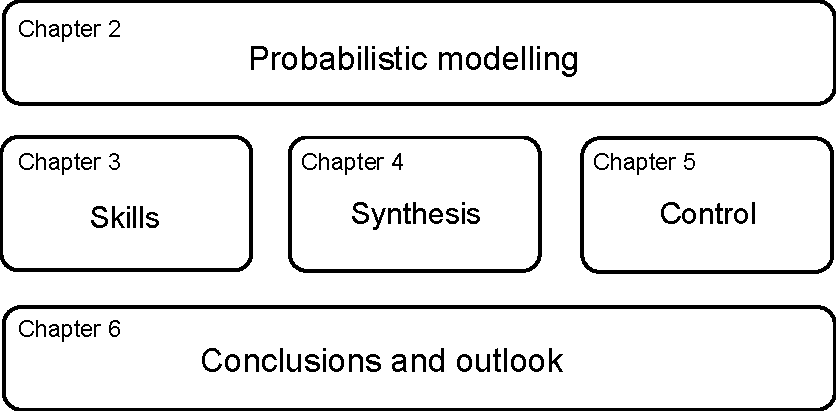
\includegraphics[width=0.7\linewidth]{outline.pdf}
\captionsetup{justification=raggedright}
\caption{Thesis outline}
\label{fig:outline}
\end{figure} 
\subsubsection{A skill framework for assembly problem exploiting arm-base coordination}
Mobile manipulators are the robots which equipped with a mobile base platform 
for navigation and arm(s) for manipulation. For reach-and-grasp tasks, state-of-the-art 
approaches consider it as two isolated problems: a navigation problem followed by a motion 
planning problem. Using these approaches a robot should first move its mobile platform 
to a location that the object is reachable, then use its manipulator to accomplish the object grasping task. Although it is a feasible solution, the time used to perform this task is not efficient. In contrast, a human performs the same task with all his actuation capability (arm, hand, body, locomotion) in a coordinated manner. In chapter~\ref{chapter4}, inspired by the human, we propose to bridge the gap between human reach-and-grasping and robotic reach- 
and-grasping by arm-platform coordination. An analysis of the reachability 
of a mobile manipulator is first conducted. The result revealed that the overlap between 
the workspace of a manipulator with the observation space of a fixed mounted camera is 
very limited. As a result, a mobile manipulator has to  face the following dilemma usually, 
the target object is located in the field of view of the robot, but it is not reachable from 
the robot manipulator, or the object is reachable from the manipulator but lies out of 
the field of view of the robot. This situation implies that arm-platform coordination is the only 
promising approach to solve the reach-and-grasping problem efficiently. To enable a mobile 
manipulator to move with its full degree of freedom (DOF), we propose a concept of 
virtual joints as well as a virtual kinematic chain. The virtual kinematic chain is composed of both the 
manipulators' joints and virtual joints. In this way, the planning of the arm- 
platform coordinated motion can be seamlessly integrated into an existing motion planning 
framework. We demonstrate the benefits of this concept in an assembly problem and propose a skill-based framework to solve the problem in a generalizable fashion. In this framework, reusable high-level skills can be parametrized to perform pick, place and insert operations. The high-level skills can reason about where to grasp the object so that the constraints for place and insert operation are satisfied. Fig.~\ref{fig:skill_over_view} illustrates the input and output of the system.
\begin{figure}[!htbp]
\centering
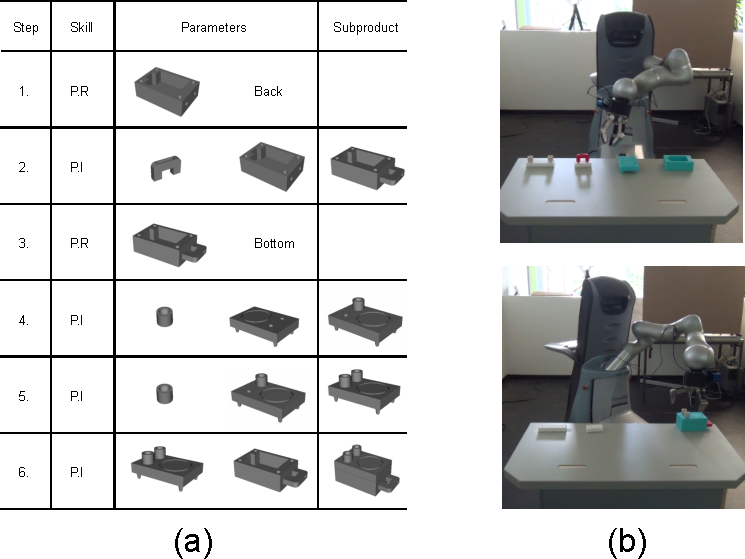
\includegraphics[width=0.8\linewidth]{skills_overview.pdf}
\captionsetup{justification=raggedright}
\caption{(a) A high-level assembly sequence provided to the system. P.R: The skill for picking and placing an object in another orientation. P.I: The skill for picking an object and inserting in another one. (b) A mobile manipulation robot performs the assembly task autonomously.}
\label{fig:skill_over_view}
\end{figure} 
\subsubsection{A probabilistic approach to the grasp synthesis for unknown objects }
The uncertainty of the real world, dynamics of objects and error in a perceptional 
system makes a robot difficult to guarantee that a grasp action will always lead to a 
success. To manage the complexity and uncertainty in the real world, modeling the success probability of a grasping action is a promising method to handle these problems. In chapter~\ref{chapter:gs}, the success probability is calculated based on a model of conditional grasping success and a model of object posterior. This method reduces the complexity of directly modeling the grasp success probability. It splits a complex model into two independent models which are not correlated with each other. The conditional grasping success model describes the probability of success by taken an action, under the condition that the object state is given. It is modelled using four criteria, which maps the principle of underlying grasp physics, actuation error and representation uncertainty to the model. Object posterior models the object state distribution after a series of observations are obtained. Depending on the choice of the representation, for some real world objects whose shape can be approximated by a group of shape primitives, the dimension of the object state space is small. The object posterior of these objects can be computed by e.g. Bayes filtering. For most real world objects, the dimension of state space is large because of their individual courses of the surface. We propose a new surface representation and a fusion method to compute the object posterior. The underlying structure of the surface representation is a variance augmented signed distance function. This representation allows temporal and spatial fusion by multiple depth cameras with individual noise characteristics. The result of the sensor fusion is a uncertainty-aware surface distribution which approximates the object posterior. After modeling the grasp success probability, the aim is to search for a grasp action that maximizes the success probability. For this purpose, we propose a simulated annealing method to find a feasible grasp. This approach seamlessly connects grasp perception and grasp control in a systematic way, while serves as a foundation for grasping unknown objects. The computational time of our method performs 30 times faster than a state-of-the-art method which uses a similar representation. Experimental results verify a significant grasping accuracy improvement in the scenario of grasping real world unknown objects by using the proposed method. Fig.~\ref{fig:synthesis_overview} elaborates some detail of proposed  method. 
\begin{figure}[!htbp]
\centering
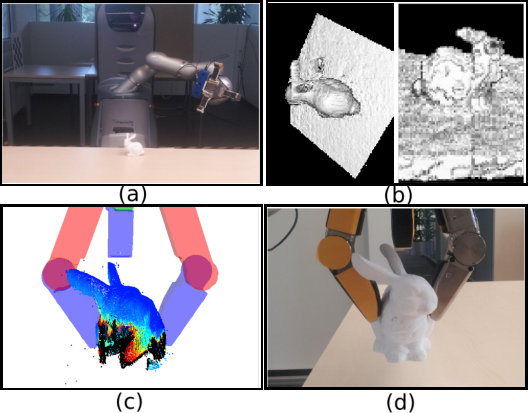
\includegraphics[width=0.8\linewidth]{synthesis_overview.pdf}
\captionsetup{justification=raggedright}
\caption{(a) The object is presented to the robot for the first time. (b) The robot reconstructs the object surface by fusing sensor measurement from two depth cameras. (c) An uncertainty-aware object model is constructed and a feasible grasp is found for grasping the object. (d) Successful execution of the grasp on a real robot.}
\label{fig:synthesis_overview}
\end{figure} 
\subsubsection{An adaptive control architecture for closed-loop grasp execution}
Chapter~\ref{chapter_control} addresses the control aspect of the grasping process. In general, individual actuators of a mobile manipulator are usually controlled by their independent interface. However, arm-platform coordination requires control commands to be sent to each actuator simultaneously. To control the individual actuators in synchrony, we propose a system control architecture, which enables a plug-in mechanism to combine arbitrary independent actuators into a standard control loop in a flexible manner. This allows a mobile manipulator to easily switch and combine the actuators according to the requirements of a grasping phase. For example, a mobile manipulator can use arm-platform coordination in the pre-grasp phase for moving to a reachable position and for interacting with an object. Motions executed by the arm alone can be employed in the grasp-motion phase for approaching a grasp configuration. Arm-gripper coordination can be utilized in the force-closure phase for  stabilizing the object within the gripper. In most previous approaches, motions of the grasping are usually planned beforehand. Thus, the adaptation of the grasp motion to the change of the object state is not possible. We propose to solve this problem by an online trajectory generation algorithm and feed the state of the object back to the trajectory generator. In this way, a large control loop is closed by the system. Using the proposed method, a mobile manipulator is not only able to reason about the grasp configuration but also recognize the change of the environment and adapt to the change. As a result, the robustness of the grasping accuracy is significantly improved. In Fig.~\ref{fig:control_overview}, the robot uses the proposed method to grasp light objects. 
\begin{figure}[!htbp]
\centering
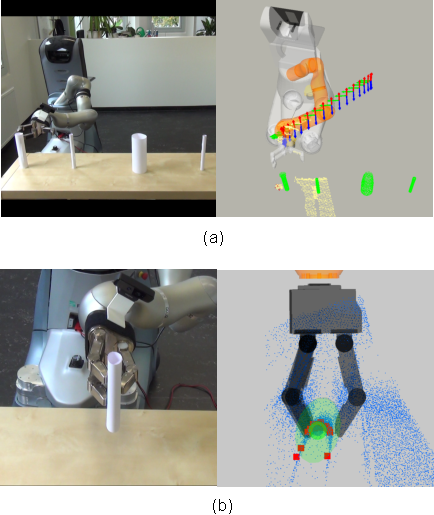
\includegraphics[width=0.6\linewidth]{control_overview.pdf}
\captionsetup{justification=raggedright}
\caption{(a) The robot is about to grasp light objects. The radius and position of the objects are estimated online during the reach-to-grasp phase. (b) The robot successfully pick up the object despite of large sensing uncertainty.}
\label{fig:control_overview}
\end{figure} 

%\subsubsection{Probabilistic modeling and Maximization of Grasping Success}
%Uncertainty of the real world, unknown dynamics of objects and error in a perceptional system makes a robot difficult to guarantee that a grasp action will  always lead to a success. To manage the complexity and uncertainty in the real world, modeling the success probability of a grasping action is a promising method to handle these problems. In Chapter 3 we describe a probabilistic approach to model the grasping process. The success probability is calculated based on a model of conditional grasping success and a model of object posterior. This method reduces the complexity of directly modeling the grasp success probability. It splits a complex modeling problem into two independent models which are not correlated with each other. The conditional grasp success model describes the probability of success by taken an grasp action, under the condition that the object state is given. It is modelled using four criteria, which maps the principle of underlying grasp physics, actuation uncertainty, representation uncertainty and a task  affordance to the model. Object posterior models the object state distribution after a series of observations are conducted. Depending on the choice of the representation, for some real world objects whose shape can be approximated by a group of shape primitives, the dimension of the object state space is small. The object posterior of these objects can be computed by e.g. Bayes filtering. For most real  world objects, the dimension of state space is large because of their individual courses of the surface, we propose a new surface representation and fusion method to compute the posterior. The underlying structure of the surface representation is a variance augmented signed distance function. This representation allows temporal and spacial fusion by multiple depth cameras with  individual noise characteristics. The result of the sensor fusion is a uncertainty-aware surface distribution which approximate the object posterior. After modeling the grasp success probability, the aim  is to search for a grasp action that maximizes the success probability. For this purpose, we propose a Monte Carlo based method to find an optimal grasp trajectory. This method seamlessly connects grasp perception and grasp control in a systematic way, while serves as a foundation for grasping unknown objects. The computational time of our method performs 30 times faster than the state-of-the-art. Experimental results verifies a significant grasping accuracy improvement in the scenario of  grasping real world unknown objects by using the proposed method. 
%
%
%\subsubsection{Arm-platform Coordination Enables Realizing Grasping Strategy and Efficient Mobile Manipulation}
%Mobile manipulators are the robots which typically equipped with a mobile base platform for navigation and arm(s) for manipulation. For reach-and-grasp tasks, state-of-the-art approaches consider it as two isolated problems: a navigation problem followed by a motion planning problem. Using these approaches a robot should first move with mobile platform to a location that the object is reachable, then use its manipulator to accomplish the object grasping task. Although it is a feasible solution, the time used to perform this task is not efficient. In contrast, a human performs the same task with all his actuation capability (arm, hand, body, locomotion) in a coordinated manner. In chapter 4, inspired by the human, we propose to bridge the gap between human reach-and-grasping and robotic reach-and-grasping by arm-platform coordination. In this chapter, an analysis of the reachability of a mobile manipulator is first conducted. The result revealed that the overlap between the workspace of a manipulator with the observation space of a fixed mounted camera is very limited. As a result, a mobile manipulator has to usually face the following dilemma, the target object is located in the field of view of the robot, but it is not reachable from the robot manipulator, or the object is reachable from the manipulator but lies out of the field of view of the robot. This implies that arm-platform coordination is the only promising approach to  efficiently solve the reach-and-grasping problem. To enable a mobile manipulator to move with its whole degree of freedom (DOF), we propose a concept of virtual joints, and add another kinematic structure by composing the virtual joints and the manipulators' joints into a common kinematic chain. In this way, the planning of the arm-platform coordinated motion can be seamless integrated into an existing motion planning framework. We demonstrate the benefits of this concept in two problems: grasp strategy planning and assembly task planning. In grasp strategy planning, we propose to design several strategies for the grasping process. Some are indented for reducing perceptual uncertainty, others are better for increasing grasp efficiency. A strategy selection algorithm based on Markov Decision Process is proposed to handle which strategy should be selected. In assembly task planning, two high-level assembly skills are designed to encapsulate low-level perception and motion planning tasks. A base-position planning algorithm based on iterative inverse kinematic is proposed to compute the optimal base placement to solve the aforementioned dilemma. The concept of arm-platform coordination allows a complex grasp strategy being executable in the strategy planning problem while improves the task efficiency for complex assembly problems.   
%
%
%\subsubsection{Boosting Grasping Robustness and Flexibility by an Adaptive Control Architecture}
%After the concept of arm-platform coordination is introduced in chapter 4. Chapter 5 addresses the control aspect of the grasping process. In general, individual actuators of a mobile manipulator are usually controlled by their independent interface. However, arm-platform coordination requires control commands to be sent to each actuator simultaneously. To control the individual actuators in synchrony, we propose a system control architecture, which enables a plug-in mechanism to combine arbitrary independent actuators into a common control loop in a flexible manner. This allows a mobile manipulator to easily switch and combine the actuators according to the requirements of a grasping phase. For example, a mobile manipulator can use arm-platform coordination in the pre-grasp phase for moving to a reachable position and for interacting with an object. Motions executed by arm alone can be used in the grasp-motion phase for approaching a grasp configuration. Arm-gripper coordination can be exploited in the force-closure phase for stabilizing the object within the gripper. 
%
%In the most state-of-the-art grasping approaches, motions of the grasping are usually pre-planned. Thus, adaptation of the grasp motion to the change of the object state is not possible. We propose to solve this problem by an online trajectory generation algorithm and feed the state of the object back to the trajectory generator. In this way, a large control loop is closed for the system. Using the proposed method, a mobile manipulator is not only able to reason about the grasp configuration  but also recognize the change of the environment and adapt to the change. As a result, the robustness of the grasping accuracy is significant improved. 

 


\cleardoublepage
\thispagestyle{empty}
%chapter 2
\chapter{A Probabilistic Graphic Model for Grasping Problem}
\label{chapter2}
\section{Introduction}
As we mentioned in the previous chapter, the essence of the robotic grasping problem is to control the actuators to achieve grasping success. Due to the process uncertainty, the same measurement and the same actuator control may not result in the same outcome.  A lot of uncertain factors are involved in the grasping process. These include imperfect sensor input, the shape of an object, precision of control and satisfaction of task constraints.  These include sensor measurement, shape of object, precision of control and satisfaction of task constraints. They are all influence factors contributing to a grasp success. Therefore, it is more reasonable to use a probabilistic model to estimate the probability of grasp success rather than using a deterministic model. As the success probability of grasping depends on many factors, direct modeling the problem from the factors to success probability is complex and hard. One way to handle the complexity is to model the grasping problem using probabilistic graphic models~\cite{Koller1989}.  

Probabilistic graphic models use a graph structure to represent a probabilistic distribution over high dimensional space. The major advantage of using a graph-based representation is one can break the modeling of complex probability distribution over every possible variable into simple small factors. The joint distribution of every possible variable is simply the multiplication of these small factors. Specifically,  we can break up the modeling of joint distribution over all the factors which may influence the success into smaller manageable probability models.  We use one family of the probabilistic graphic models called `Bayesian Networks' to model the grasping problem. The `Bayesian Networks' uses a directed graph to represent    the probability distribution. A directed graph is composed of a set of nodes and directed edges. The nodes specify random variables that represent influence factors. The edges define the direction of dependency between factors. The reader can refer to~\cite{Korb2003} for a more formal description of  `Bayesian Networks.'  


\section{Probabilistic modeling of grasping using Bayesian networks}
In this section, we introduce a general description for grasping problems using a Bayesian network. We first define a set of variables for the problem. A graph is then proposed to model the dependency between the variables. Then we explain that solving grasping problems is equivalent to solving inference tasks under the condition that a subset of the defined variables is observed.   
\subsection{Variable definition and graph structure}
The first variable that we define for the grasping problem is the outcome of a grasping process $S$. The outcome is a discrete random variable which takes two values to specify whether a grasping process succeeds or not. One standard definition of the success is whether the gripper of a robot achieves force closure on the object. However, this definition only considers the result of grasp acquisition itself. As grasping of an object may also have a purpose, the task intention of a grasp should also be considered as a part of grasp success. Therefore, we define the success of a grasping process not only based on force closure property but also on whether the task constraint is fulfilled. Thus, we define another two discrete variables $F$ for whether the gripper achieves force closure condition and $C$ for whether constraints defined by the grasping task is fulfilled. Consequently, the outcome of a grasping process $S$ only depends on $F$ and $C$. Now let's consider which factors can influence the force closure condition $F$. It is reasonable to think that object state $X$ and robot controls $U$ jointly affect the force closure condition. As the object state $X$ is normally not observable and derived from the sensor measurement, we define $Z$ to be the sensor measurement that can influence the estimation of object state. The task constraint satisfaction $C$ represents whether a grasp configuration satisfies the condition regarding a specified task. Therefore, a task specification $T$ naturally influences the task constraint. Besides that without the grasp configuration, it is not possible to evaluate whether task constraint is fulfilled or not. Therefore, $C$ is also dependent on object state $X$ and robot control $U$.  

Based on the analysis of the factors and their dependencies we can model the  relationships of the factors into a Bayesian network. Figure.~\ref{fig:bnet} depicts the proposed network that we define for the grasping problem. All the variables surrounded by a box are binary-valued discrete variables, while the variables surrounded by an ellipse indicate their domain can be either discrete or continuous. All the defined variables are summed up in Tab.~\ref{tab:random_variable}.

\begin{figure}[!htbp]
\centering
%\def\svgwidth{0.6\linewidth}
%%% Creator: Inkscape inkscape 0.48.4, www.inkscape.org
%% PDF/EPS/PS + LaTeX output extension by Johan Engelen, 2010
%% Accompanies image file 'baysianmodel.pdf' (pdf, eps, ps)
%%
%% To include the image in your LaTeX document, write
%%   \input{<filename>.pdf_tex}
%%  instead of
%%   \includegraphics{<filename>.pdf}
%% To scale the image, write
%%   \def\svgwidth{<desired width>}
%%   \input{<filename>.pdf_tex}
%%  instead of
%%   \includegraphics[width=<desired width>]{<filename>.pdf}
%%
%% Images with a different path to the parent latex file can
%% be accessed with the `import' package (which may need to be
%% installed) using
%%   \usepackage{import}
%% in the preamble, and then including the image with
%%   \import{<path to file>}{<filename>.pdf_tex}
%% Alternatively, one can specify
%%   \graphicspath{{<path to file>/}}
%% 
%% For more information, please see info/svg-inkscape on CTAN:
%%   http://tug.ctan.org/tex-archive/info/svg-inkscape
%%
\begingroup%
  \makeatletter%
  \providecommand\color[2][]{%
    \errmessage{(Inkscape) Color is used for the text in Inkscape, but the package 'color.sty' is not loaded}%
    \renewcommand\color[2][]{}%
  }%
  \providecommand\transparent[1]{%
    \errmessage{(Inkscape) Transparency is used (non-zero) for the text in Inkscape, but the package 'transparent.sty' is not loaded}%
    \renewcommand\transparent[1]{}%
  }%
  \providecommand\rotatebox[2]{#2}%
  \ifx\svgwidth\undefined%
    \setlength{\unitlength}{266.48922058bp}%
    \ifx\svgscale\undefined%
      \relax%
    \else%
      \setlength{\unitlength}{\unitlength * \real{\svgscale}}%
    \fi%
  \else%
    \setlength{\unitlength}{\svgwidth}%
  \fi%
  \global\let\svgwidth\undefined%
  \global\let\svgscale\undefined%
  \makeatother%
  \begin{picture}(1,0.7093861)%
    \put(0,0){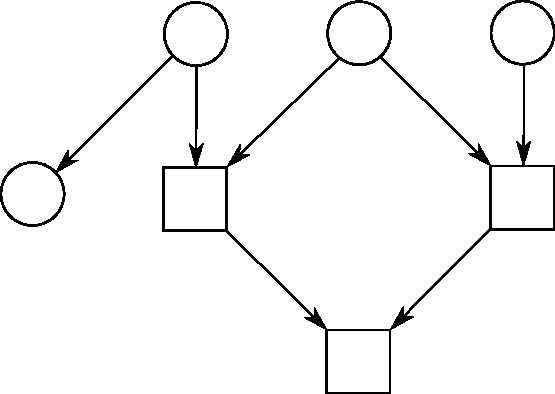
\includegraphics[width=\unitlength]{baysianmodel.pdf}}%
    \put(0.62968498,0.04171382){\color[rgb]{0,0,0}\makebox(0,0)[lb]{\smash{$S$}}}%
    \put(0.33638551,0.33553136){\color[rgb]{0,0,0}\makebox(0,0)[lb]{\smash{$F$}}}%
    \put(0.92239445,0.33553136){\color[rgb]{0,0,0}\makebox(0,0)[lb]{\smash{$C$}}}%
    \put(0.33586739,0.63038521){\color[rgb]{0,0,0}\makebox(0,0)[lb]{\smash{$X$}}}%
    \put(0.62968498,0.63149328){\color[rgb]{0,0,0}\makebox(0,0)[lb]{\smash{$U$}}}%
    \put(0.92671889,0.62934899){\color[rgb]{0,0,0}\makebox(0,0)[lb]{\smash{$T$}}}%
    \put(0.0420857,0.34096392){\color[rgb]{0,0,0}\makebox(0,0)[lb]{\smash{$Z$}}}%
  \end{picture}%
\endgroup%

%\resizebox{1\textwidth}{!}{%% Creator: Inkscape inkscape 0.48.4, www.inkscape.org
%% PDF/EPS/PS + LaTeX output extension by Johan Engelen, 2010
%% Accompanies image file 'graphicalModel_temporal.pdf' (pdf, eps, ps)
%%
%% To include the image in your LaTeX document, write
%%   \input{<filename>.pdf_tex}
%%  instead of
%%   \includegraphics{<filename>.pdf}
%% To scale the image, write
%%   \def\svgwidth{<desired width>}
%%   \input{<filename>.pdf_tex}
%%  instead of
%%   \includegraphics[width=<desired width>]{<filename>.pdf}
%%
%% Images with a different path to the parent latex file can
%% be accessed with the `import' package (which may need to be
%% installed) using
%%   \usepackage{import}
%% in the preamble, and then including the image with
%%   \import{<path to file>}{<filename>.pdf_tex}
%% Alternatively, one can specify
%%   \graphicspath{{<path to file>/}}
%% 
%% For more information, please see info/svg-inkscape on CTAN:
%%   http://tug.ctan.org/tex-archive/info/svg-inkscape
%%
\begingroup%
  \makeatletter%
  \providecommand\color[2][]{%
    \errmessage{(Inkscape) Color is used for the text in Inkscape, but the package 'color.sty' is not loaded}%
    \renewcommand\color[2][]{}%
  }%
  \providecommand\transparent[1]{%
    \errmessage{(Inkscape) Transparency is used (non-zero) for the text in Inkscape, but the package 'transparent.sty' is not loaded}%
    \renewcommand\transparent[1]{}%
  }%
  \providecommand\rotatebox[2]{#2}%
  \ifx\svgwidth\undefined%
    \setlength{\unitlength}{514.815004bp}%
    \ifx\svgscale\undefined%
      \relax%
    \else%
      \setlength{\unitlength}{\unitlength * \real{\svgscale}}%
    \fi%
  \else%
    \setlength{\unitlength}{\svgwidth}%
  \fi%
  \global\let\svgwidth\undefined%
  \global\let\svgscale\undefined%
  \makeatother%
  \begin{picture}(1,0.36762093)%
    \put(0,0){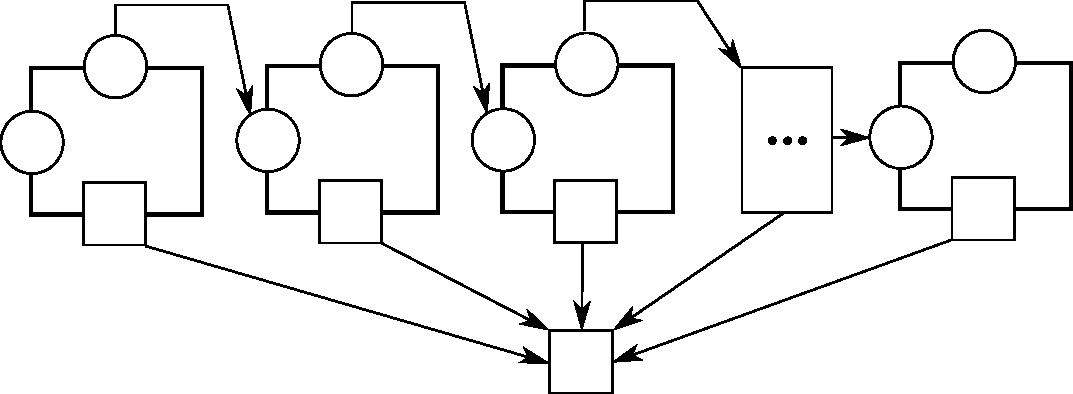
\includegraphics[width=\unitlength]{graphicalModel_temporal.pdf}}%
    \put(0.09547193,0.29665535){\color[rgb]{0,0,0}\makebox(0,0)[lb]{\smash{$U_0$}}}%
    \put(0.09407952,0.15956687){\color[rgb]{0,0,0}\makebox(0,0)[lb]{\smash{$S_0$}}}%
    \put(0.01881458,0.22563278){\color[rgb]{0,0,0}\makebox(0,0)[lb]{\smash{$Z_0$}}}%
    \put(0.31237857,0.29852096){\color[rgb]{0,0,0}\makebox(0,0)[lb]{\smash{$U_1$}}}%
    \put(0.31409408,0.16143247){\color[rgb]{0,0,0}\makebox(0,0)[lb]{\smash{$S_1$}}}%
    \put(0.23882916,0.22749837){\color[rgb]{0,0,0}\makebox(0,0)[lb]{\smash{$Z_1$}}}%
    \put(0.90558919,0.30139354){\color[rgb]{0,0,0}\makebox(0,0)[lb]{\smash{$U_n$}}}%
    \put(0.90419676,0.16430507){\color[rgb]{0,0,0}\makebox(0,0)[lb]{\smash{$S_n$}}}%
    \put(0.82893184,0.23037096){\color[rgb]{0,0,0}\makebox(0,0)[lb]{\smash{$Z_n$}}}%
    \put(0.53050271,0.02213156){\color[rgb]{0,0,0}\makebox(0,0)[lb]{\smash{$S_f$}}}%
    \put(0.53175169,0.29895161){\color[rgb]{0,0,0}\makebox(0,0)[lb]{\smash{$U_2$}}}%
    \put(0.53346717,0.16186314){\color[rgb]{0,0,0}\makebox(0,0)[lb]{\smash{$S_2$}}}%
    \put(0.4582022,0.22792902){\color[rgb]{0,0,0}\makebox(0,0)[lb]{\smash{$Z_2$}}}%
  \end{picture}%
\endgroup%
}
\resizebox{.5\textwidth}{!}{%% Creator: Inkscape inkscape 0.48.4, www.inkscape.org
%% PDF/EPS/PS + LaTeX output extension by Johan Engelen, 2010
%% Accompanies image file 'baysianmodel.pdf' (pdf, eps, ps)
%%
%% To include the image in your LaTeX document, write
%%   \input{<filename>.pdf_tex}
%%  instead of
%%   \includegraphics{<filename>.pdf}
%% To scale the image, write
%%   \def\svgwidth{<desired width>}
%%   \input{<filename>.pdf_tex}
%%  instead of
%%   \includegraphics[width=<desired width>]{<filename>.pdf}
%%
%% Images with a different path to the parent latex file can
%% be accessed with the `import' package (which may need to be
%% installed) using
%%   \usepackage{import}
%% in the preamble, and then including the image with
%%   \import{<path to file>}{<filename>.pdf_tex}
%% Alternatively, one can specify
%%   \graphicspath{{<path to file>/}}
%% 
%% For more information, please see info/svg-inkscape on CTAN:
%%   http://tug.ctan.org/tex-archive/info/svg-inkscape
%%
\begingroup%
  \makeatletter%
  \providecommand\color[2][]{%
    \errmessage{(Inkscape) Color is used for the text in Inkscape, but the package 'color.sty' is not loaded}%
    \renewcommand\color[2][]{}%
  }%
  \providecommand\transparent[1]{%
    \errmessage{(Inkscape) Transparency is used (non-zero) for the text in Inkscape, but the package 'transparent.sty' is not loaded}%
    \renewcommand\transparent[1]{}%
  }%
  \providecommand\rotatebox[2]{#2}%
  \ifx\svgwidth\undefined%
    \setlength{\unitlength}{266.48922058bp}%
    \ifx\svgscale\undefined%
      \relax%
    \else%
      \setlength{\unitlength}{\unitlength * \real{\svgscale}}%
    \fi%
  \else%
    \setlength{\unitlength}{\svgwidth}%
  \fi%
  \global\let\svgwidth\undefined%
  \global\let\svgscale\undefined%
  \makeatother%
  \begin{picture}(1,0.7093861)%
    \put(0,0){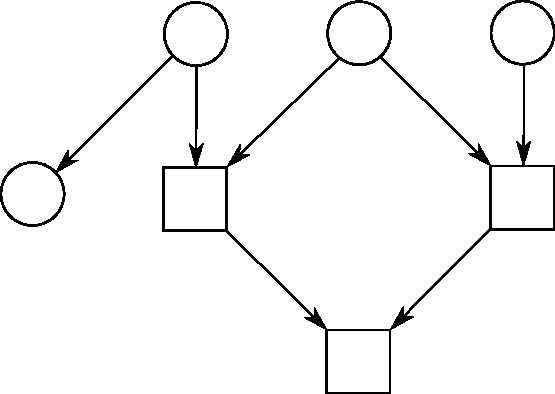
\includegraphics[width=\unitlength]{baysianmodel.pdf}}%
    \put(0.62968498,0.04171382){\color[rgb]{0,0,0}\makebox(0,0)[lb]{\smash{$S$}}}%
    \put(0.33638551,0.33553136){\color[rgb]{0,0,0}\makebox(0,0)[lb]{\smash{$F$}}}%
    \put(0.92239445,0.33553136){\color[rgb]{0,0,0}\makebox(0,0)[lb]{\smash{$C$}}}%
    \put(0.33586739,0.63038521){\color[rgb]{0,0,0}\makebox(0,0)[lb]{\smash{$X$}}}%
    \put(0.62968498,0.63149328){\color[rgb]{0,0,0}\makebox(0,0)[lb]{\smash{$U$}}}%
    \put(0.92671889,0.62934899){\color[rgb]{0,0,0}\makebox(0,0)[lb]{\smash{$T$}}}%
    \put(0.0420857,0.34096392){\color[rgb]{0,0,0}\makebox(0,0)[lb]{\smash{$Z$}}}%
  \end{picture}%
\endgroup%
}
\captionsetup{justification=raggedright}
\caption{A Bayesian network for the grasping problem. Variables surrounded by a box are binary-valued discrete random variables. Variables surrounded by an circle can be either continuous or discrete.}
\label{fig:bnet}
\end{figure}	

\begin{table}[!htbp]
\centering
\begin{tabular}{cl}
Variable & Description                              \\
$S$      & outcome of a grasping process            \\
$F$      & satisfaction of force closure condition \\
$U$      & robot control                            \\
$Z$      & sensor measurement                       \\
$X$      & object state                             \\
$T$      & task specification                       \\
$C$      & satisfaction of task constraints       
\end{tabular}
\caption{Definition of variables }
\label{tab:random_variable}
\end{table}

Based on the proposed Bayesian network, the joint distribution of all the variables can be written according to the graph structure. The joint distribution of the grasping problem is given by 
\begin{equation}
\begin{split}
\pr (S,F,C,X,Z,U,T) = & \pr (S | F, C )\cdot \pr(F| X,U) \cdot \pr(C | U,T) \cdot \pr(Z|X) \\ 
  &\cdot \pr(X) \cdot \pr (U) \cdot \pr(T)
\end{split}
\label{equ:joint_distribution_grasp}
\end{equation} 
where $\pr (S | F, C )$ , $\pr(F| X,U)$ , $\pr(C | U,T)$ and $\pr(Z|X)$ are conditional probability distributions (CPD). Among them, the CPD of  $\pr (S | F, C )$  can be expressed  using a CPD table, because all the variables involved are discrete. The outcome $S$ of a grasping process is success, if and only if $F$ is success and $C$ is success. Therefore, the CPD of $\pr (S | F, C )$ is directly given by Tab.~\ref{tab:cpd}. The CPD of $\pr(F|X,U)$ specifies the probability of force closure. The modeling of this CPD depends on which representation of $X$ and of $U$ are used. $\pr(C | U,T)$ models the probability of task constraint satisfaction.  $P(Z|X) $ models the probability distribution of $Z$ given the object $X$, which is per definition the measurement model of a sensor. $\pr(X)$, $\pr(U)$ and $\pr(T)$ are the prior distributions respectively. 

\begin{table}[!htbp]
\centering
\begin{tabular}{|l|r|r|}
\hline
& $s^0$ & $s^1$ \\ \hline
$f^0, c^0$ & 1     & 0     \\ \hline
$f^0, c^1$ & 1     & 0     \\ \hline
$f^1, c^0$ & 1     & 0     \\ \hline
$f^1, c^1$ & 0     & 1     \\ \hline
\end{tabular}
\caption{The conditional probability distribution for $\pr (S | F, C )$. The superscript 1 and 0 indicate the variable equals success or failure respectively.}
\label{tab:cpd}
\end{table}

\subsection{Query of conditional probability distribution}
One of the advantages of using probabilistic graphical models is we can perform inference tasks. The goal of an inference task is to query the probability of a set of variables based on a set of observed evidence. Mathematically, let $Y$ be a set of variables for the query, $E = e$ be a set of evidence. The inference task is to compute the conditional probability  distribution of $Y$ given $E$. The conditional probability distribution is given by 
\begin{equation}
\pr (Y|E = e) =  \frac{\pr (Y, E = e)} {\pr (E = e)}
\end{equation}
In the context of our grasping problem, the evidence variables are measurement $Z$, robot controls $U$ and task specifications $T$. The probability distribution that most interests us is $\pr(S | Z, U, T) $, the outcome of a grasping process given the evidence variables. The query of the probability gives how likely a grasp will succeed. Then, the goal of grasping is to maximize the probability of success $\pr(S = 1 | Z, U, T) $. Among the evidence in this probability, $Z$ is measurement given by the sensor and $T$ is given by the task, the only variable that can be changed to maximize the success probability is the robot control $U$. Therefore, the grasping problem is defined by find the best robot control $U = u^*$, so that the conditional probability $\pr(S = 1 | Z = z', U=u^* , T = t') $ is maximized: 
\begin{equation}
 u^* = \argmax_{u} \pr (S = 1| Z , U ,T)  
\label{equ:argmax_probS}
\end{equation}

\section{Inference in different grasping scenarios}
So far we propose a coherent probabilistic model to describe the grasping problem. In reality, the objects to be grasped, the type of sensor used for perception and the type of gripper jointly determine the hardness of a grasping problem. Hence, the representation of the random variables and the modeling of the conditional probability distribution can vary with the condition of a grasping problem. In the following sections, we elaborate how we configure the model in different grasping scenarios. 

\subsection{Grasping known objects under task constraints}
In chapter \ref{chapter4}, we consider the assembly as our target application scenario. In this scenario, since object models are given prior to grasping, the robot can use the object models for grasp planning and perception. Specific task constraints are defined for the objects, so grasping of an object is always related to a purpose. The robot has to infer the control to ensure that a specific manipulation task can be performed after grasping. Since grasping of known objects has been well studied in the previous research, we manually specify a set of force closure grasps to the object. In this way, we are allowed to condition the random variable $F=1$ to assume that the force closure is already fulfilled. The conditional probability of success in this scenario can be reformulated by 
\begin{equation}
\pr (S = 1| Z, U ,T) = \pr(S = 1|Z=z,U=u,T=t, F=1). 
\end{equation}
Similar to the previous derivation, the conditional probability of success can be expanded using Bayes rule and is expressed by 
\begin{equation}
\pr (S = 1| Z, U ,T, F = 1) =  \frac{\pr(S = 1, z, u, t, f)}{\pr(z,u,t,f)}.  
\label{equ:query_prob_condition_f}
\end{equation}
We can further compute the nominator of the Equ.~\ref{equ:query_prob_condition_f} by marginalizing $C$ and $X$ given by 
\begin{equation}
\begin{split}
\pr(S = 1, z, u, t, f) &= \sum_{C,X} \pr (S=1,C,X,z,u,t,f)  \\
                       &= \sum_{X}  \pr (S=1, C = 0, X, z,u,t,f) + \sum_{X} \pr(S=1,C=1,X,z,u,t,f).
\end{split}
\label{equ:marginalization_task}
\end{equation}
Similar as in the equation \ref{equ:elimination}, the first term of equation~\ref{equ:marginalization_task} also equals zero, because the conditional probability of success given the evidence $\pr(S|C=0)$ is zero according to Tab.~\ref{tab:cpd}. The second term can be further expressed by   
\begin{equation}
\begin{split}
 \pr(S = 1, z, u, t, f)  = & \sum_{X} \pr(S=1,C=1,X,z,u,t,f)  \\
 					    =& \sum_{X} \pr (S=1|F=1,C=1) \cdot \pr(F = 1|X,u)\cdot\pr(z|X) \\
 					     &\cdot \pr(C=1|u,t) \cdot \pr(X) \cdot \pr(u) \cdot \pr(t) \\
 					    =&\sum_{X} \pr(C=1|u,t) \cdot\pr(z|X) \cdot \pr(X) \cdot \pr(u) \cdot \pr(t). \\ 
\end{split}
\end{equation}
Now we can replace the term $\pr(z|X) \cdot \pr(X)$ by  $\pr(X|z)\cdot\pr(z)$ using Bayes rule and moves the sum product before $\pr(X|z)$. The joint probability is then given by  
\begin{equation}
\begin{split}
 \pr(S = 1, z, u, t, f) = \pr(C=1|u,t) \cdot \sum_{X} \pr(X|z)\cdot\pr(z) \cdot \pr(u) \cdot \pr(t).
\end{split}              
\end{equation}
With $\sum_{X} \pr(X|z) = 1$ and $\pr(z) \cdot \pr(u) \cdot \pr(t)$ is equal to a normalization constant $\eta'''$. We can write the joint probability further by 
\begin{equation}
\begin{split}
 \pr(S = 1, z, u, t, f) = \eta''' \cdot  \pr(C=1|u,t). 
\end{split}              
\end{equation}
Combining the denominator which is also a normalization constant, the final conditional probability which we want to query is simplified to 
\begin{equation}
\begin{split}
 \pr(S = 1 | Z, U, T, F  = 1) =& \frac{\eta''' \cdot  \pr(C=1|u,t)}{\pr(z,u,t,f)} \\
     						  =& \eta'''' \cdot  \pr(C=1 | u,t). 
\end{split}              
\end{equation}
Therefore, the problem of grasping known objects with task constraints is defined by finding the best robot control $U=u^*$, so that the conditional probability of satisfying the task constraints is maximized.  
\begin{equation}
  u^* = \argmax_{u} \pr(C=1 | u,t)  
\end{equation}

  
\subsection{Grasping unknown objects} 
In chapter \ref{chapter:gs}, we consider the scenario of grasping unknown objects. In this case, no information about the objects is available in prior. The robot neither knows the geometry nor the pose of an object. In this scenario only `Pick and place' is one of the reasonable tasks. Since there is no information about object's geometry, the orientation of an object can be chosen arbitrarily for a placing task. It is reasonable to assume that the task constraint is already fulfilled. Therefore, we can condition an additional variable in the set of evidence by setting $C = 1$. Based on the graphical model, conditioning of variable $C$ blocks the reasoning pattern from task specification $T$ to the outcome $S$, $T$ and $S$ are therefore conditional independent. The probability of success specified in Equ.~\ref{equ:argmax_probS} can be reformulated by 
\begin{equation}
\pr (S = 1| Z, U ,T) = \pr(S = 1|Z=z,U=u,T=t, C=1)
\end{equation}
where the variable $C$ now becomes an evidence. Based on the Bayes rule, the conditional probability can be further expanded by
\begin{equation}
 \pr(S = 1|Z=z,U=u,T=t,C=1) = \frac{ \pr(S = 1,z,u,c,t)}{\pr(z,u,c,t)}.
 \label{equ:bayesrule_grasp}
\end{equation}
Here we replace $C=1$ by $c$ to keep the equation concise. The nominator of Equ.~\ref{equ:bayesrule_grasp} can be computed by marginalizing the joint distribution of all the variables specified in Equ.~\ref{equ:joint_distribution_grasp}. The variables to be marginalized are neither in the set of query nor  the set of evidence. In this case, the variables to be marginalized are $X$ and $F$. Without loss of generality, we use the sum operation for marginalization by assuming all the variables are in discrete space. Later we can freely replace the sum operation by an integral if the actual representation of the variable is in continuous space. First, we eliminate the variable $F$. Since $F$ can only take 0 or 1, the result of elimination is thus given by 
\begin{equation}
\begin{split}
\pr(S = 1,z,u,c) =& \sum_{F,X} \pr (S=1,F,c,X,z,u,t)  \\
                 =& \sum_{X}  \pr (S=1, F = 0, c ,X, z,u,t) + \sum_{X}  \pr (S=1,F=1,c,X,z,u,t).                  
\end{split}
\label{equ:elimination}
\end{equation}
The first term $\pr (S=1, F = 0, c ,X, z,u,t)$ can be expanded by $ \pr (S=1|F=0,C=1) $ multiplying the rest of the factors according to Equ.~\ref{equ:joint_distribution_grasp}. The condition probability $\pr (S=1|F=0,C=1)$ is equal to zero according to Tab.~\ref{tab:cpd}, so the first term of Equ.~\ref{equ:elimination} equals zero regardless what value the rest of the factors take. So we can simplify the joint probability $\pr(S = 1,z,u,c)$ by considering only the second term by
\begin{equation}
\begin{split}
  \pr(S = 1,z,u,c) =& \sum_{X} \pr (S=1,F=1,c,X,z,u,t) \\
				    =&  \sum_{X} \pr (S=1|F=1,C=1) \cdot \pr(F = 1|X,u)\cdot\pr(z|X) \\
				    &\cdot \pr(C=1|u,t) \cdot \pr(X) \cdot \pr(u) \cdot \pr(t)
\end{split}
\label{equ:elimination2}
\end{equation}
According to Tab.~\ref{tab:cpd}, we know that the CPD of $\pr (S=1|F=1,C=1)$ equals 1. The probability of task satisfaction $P(C=1| u,t )$ also equals 1, because we assume the task constraint is always fulfilled in this scenario. The multiplication of $\pr(u) \cdot \pr(t)$ can be summarized by a constant $\eta$. The object prior $P(X)$ and the sensor model $P(z|X)$ can be summarized by $\eta' \cdot \pr(X|z)$. Thus we can simplify the Equ.~\ref{equ:elimination2} by 
\begin{equation}
\begin{split}
  \pr(S = 1,z,u,c) & = \eta \cdot \eta' \cdot \sum_{X} \pr(F = 1|X,u)\cdot \pr(X|z) 
\end{split}
\end{equation}
Now let's look at the denominator of the Equ.~\ref{equ:bayesrule_grasp}. Since the value of the denominator is also a constant $\eta''$, the conditional probability what we query for can be formulated by
\begin{equation}
\begin{split}
\pr(S = 1|Z=z,U=u,T=t,C=1) =&  \frac{\eta \cdot \eta'}{\eta''}  \cdot \sum_{X} \pr(F = 1|X,u)\cdot \pr(X|z) \\
						  & \propto  \sum_{X} \pr(F = 1|X,u)\cdot \pr(X|z).
\end{split}
\end{equation}
Therefore, the problem of grasping unknown objects is defined by finding the best robot control $U = u^*$, so that $\pr(S = 1|Z=z,U=u,T=t,C=1)$ is maximized: 
 \begin{equation}
 u^* = \argmax_{u} \sum_{X} \pr(F = 1|X,u)\cdot \pr(X|z) 
\label{equ:argmax_prob_unknown_object}
\end{equation}
The challenge in this grasping scenario can be seen from Equ.~\ref{equ:argmax_prob_unknown_object}.  The probability of force closure and the posterior probability of object state along with finding the optimal robot control are the major problems to be addressed in this scenario. 


\subsection{Grasping objects under limited sensing capability}
\label{chap:grasplimitsensing}		
% think about 2 possibility of improvement 
In chapter 5, we consider the grasping scenario in which the sensor measurement used for perception has a significant noise characteristic. Specifically, a low-cost time-of-flight depth camera is used as the primary sensor for grasping. The challenge in this scenario is how to improve the grasp success despite significant sensing uncertainty. We propose to use a camera-in-hand setup to  measure the object continuously during the grasp motion phase. The closer the distance from the camera to an object, more object detail can be measured. In this way, the uncertainty of the object can be reduced online which eventually increase the success of grasping.  

\begin{figure}[!htbp]
\centering
%\def\svgwidth{0.6\linewidth} 
%%% Creator: Inkscape inkscape 0.48.4, www.inkscape.org
%% PDF/EPS/PS + LaTeX output extension by Johan Engelen, 2010
%% Accompanies image file 'baysianmodel.pdf' (pdf, eps, ps)
%%
%% To include the image in your LaTeX document, write
%%   \input{<filename>.pdf_tex}
%%  instead of
%%   \includegraphics{<filename>.pdf}
%% To scale the image, write
%%   \def\svgwidth{<desired width>}
%%   \input{<filename>.pdf_tex}
%%  instead of
%%   \includegraphics[width=<desired width>]{<filename>.pdf}
%%
%% Images with a different path to the parent latex file can
%% be accessed with the `import' package (which may need to be
%% installed) using
%%   \usepackage{import}
%% in the preamble, and then including the image with
%%   \import{<path to file>}{<filename>.pdf_tex}
%% Alternatively, one can specify
%%   \graphicspath{{<path to file>/}}
%% 
%% For more information, please see info/svg-inkscape on CTAN:
%%   http://tug.ctan.org/tex-archive/info/svg-inkscape
%%
\begingroup%
  \makeatletter%
  \providecommand\color[2][]{%
    \errmessage{(Inkscape) Color is used for the text in Inkscape, but the package 'color.sty' is not loaded}%
    \renewcommand\color[2][]{}%
  }%
  \providecommand\transparent[1]{%
    \errmessage{(Inkscape) Transparency is used (non-zero) for the text in Inkscape, but the package 'transparent.sty' is not loaded}%
    \renewcommand\transparent[1]{}%
  }%
  \providecommand\rotatebox[2]{#2}%
  \ifx\svgwidth\undefined%
    \setlength{\unitlength}{266.48922058bp}%
    \ifx\svgscale\undefined%
      \relax%
    \else%
      \setlength{\unitlength}{\unitlength * \real{\svgscale}}%
    \fi%
  \else%
    \setlength{\unitlength}{\svgwidth}%
  \fi%
  \global\let\svgwidth\undefined%
  \global\let\svgscale\undefined%
  \makeatother%
  \begin{picture}(1,0.7093861)%
    \put(0,0){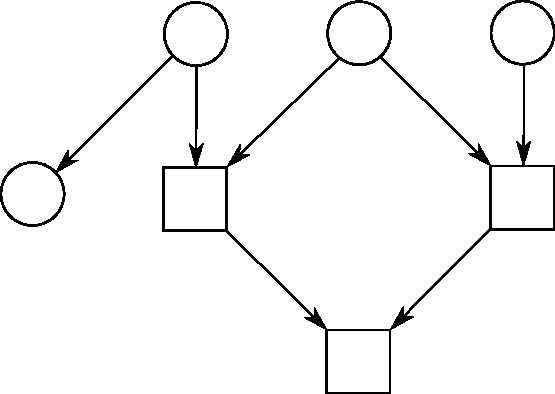
\includegraphics[width=\unitlength]{baysianmodel.pdf}}%
    \put(0.62968498,0.04171382){\color[rgb]{0,0,0}\makebox(0,0)[lb]{\smash{$S$}}}%
    \put(0.33638551,0.33553136){\color[rgb]{0,0,0}\makebox(0,0)[lb]{\smash{$F$}}}%
    \put(0.92239445,0.33553136){\color[rgb]{0,0,0}\makebox(0,0)[lb]{\smash{$C$}}}%
    \put(0.33586739,0.63038521){\color[rgb]{0,0,0}\makebox(0,0)[lb]{\smash{$X$}}}%
    \put(0.62968498,0.63149328){\color[rgb]{0,0,0}\makebox(0,0)[lb]{\smash{$U$}}}%
    \put(0.92671889,0.62934899){\color[rgb]{0,0,0}\makebox(0,0)[lb]{\smash{$T$}}}%
    \put(0.0420857,0.34096392){\color[rgb]{0,0,0}\makebox(0,0)[lb]{\smash{$Z$}}}%
  \end{picture}%
\endgroup%

\resizebox{0.5\textwidth}{!}{%% Creator: Inkscape inkscape 0.48.4, www.inkscape.org
%% PDF/EPS/PS + LaTeX output extension by Johan Engelen, 2010
%% Accompanies image file 'baysianmodel_box_model.pdf' (pdf, eps, ps)
%%
%% To include the image in your LaTeX document, write
%%   \input{<filename>.pdf_tex}
%%  instead of
%%   \includegraphics{<filename>.pdf}
%% To scale the image, write
%%   \def\svgwidth{<desired width>}
%%   \input{<filename>.pdf_tex}
%%  instead of
%%   \includegraphics[width=<desired width>]{<filename>.pdf}
%%
%% Images with a different path to the parent latex file can
%% be accessed with the `import' package (which may need to be
%% installed) using
%%   \usepackage{import}
%% in the preamble, and then including the image with
%%   \import{<path to file>}{<filename>.pdf_tex}
%% Alternatively, one can specify
%%   \graphicspath{{<path to file>/}}
%% 
%% For more information, please see info/svg-inkscape on CTAN:
%%   http://tug.ctan.org/tex-archive/info/svg-inkscape
%%
\begingroup%
  \makeatletter%
  \providecommand\color[2][]{%
    \errmessage{(Inkscape) Color is used for the text in Inkscape, but the package 'color.sty' is not loaded}%
    \renewcommand\color[2][]{}%
  }%
  \providecommand\transparent[1]{%
    \errmessage{(Inkscape) Transparency is used (non-zero) for the text in Inkscape, but the package 'transparent.sty' is not loaded}%
    \renewcommand\transparent[1]{}%
  }%
  \providecommand\rotatebox[2]{#2}%
  \ifx\svgwidth\undefined%
    \setlength{\unitlength}{286.6095bp}%
    \ifx\svgscale\undefined%
      \relax%
    \else%
      \setlength{\unitlength}{\unitlength * \real{\svgscale}}%
    \fi%
  \else%
    \setlength{\unitlength}{\svgwidth}%
  \fi%
  \global\let\svgwidth\undefined%
  \global\let\svgscale\undefined%
  \makeatother%
  \begin{picture}(1,0.78509323)%
    \put(0,0){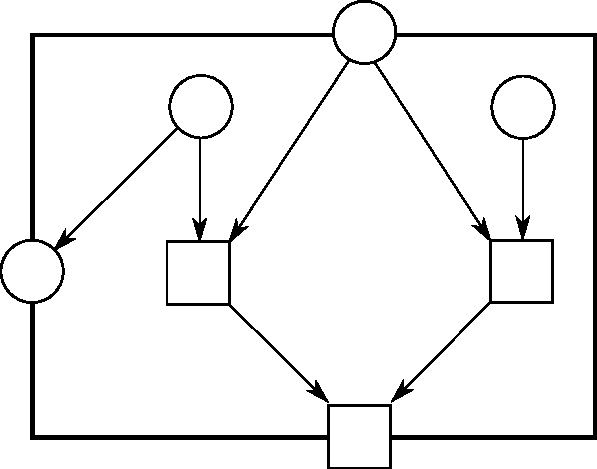
\includegraphics[width=\unitlength]{baysianmodel_box_model.pdf}}%
    \put(0.31103133,0.31530351){\color[rgb]{0,0,0}\makebox(0,0)[lb]{\smash{$F_i$}}}%
    \put(0.85906585,0.31822343){\color[rgb]{0,0,0}\makebox(0,0)[lb]{\smash{$C_i$}}}%
    \put(0.3207583,0.59357303){\color[rgb]{0,0,0}\makebox(0,0)[lb]{\smash{$X_i$}}}%
    \put(0.86459435,0.59265798){\color[rgb]{0,0,0}\makebox(0,0)[lb]{\smash{$T_i$}}}%
    \put(0.03874787,0.31903892){\color[rgb]{0,0,0}\makebox(0,0)[lb]{\smash{$Z_i$}}}%
    \put(0.58873498,0.71586238){\color[rgb]{0,0,0}\makebox(0,0)[lb]{\smash{$U_i$}}}%
    \put(0.59076283,0.03856025){\color[rgb]{0,0,0}\makebox(0,0)[lb]{\smash{$S_i$}}}%
  \end{picture}%
\endgroup%
}
\captionsetup{justification=raggedright}
\caption{Encapsulation of the original graphical model.}
\label{fig:boxmodel}
\end{figure}	
\begin{figure}[!htbp]
\centering
%\def\svgwidth{0.6\linewidth} 
%%% Creator: Inkscape inkscape 0.48.4, www.inkscape.org
%% PDF/EPS/PS + LaTeX output extension by Johan Engelen, 2010
%% Accompanies image file 'baysianmodel.pdf' (pdf, eps, ps)
%%
%% To include the image in your LaTeX document, write
%%   \input{<filename>.pdf_tex}
%%  instead of
%%   \includegraphics{<filename>.pdf}
%% To scale the image, write
%%   \def\svgwidth{<desired width>}
%%   \input{<filename>.pdf_tex}
%%  instead of
%%   \includegraphics[width=<desired width>]{<filename>.pdf}
%%
%% Images with a different path to the parent latex file can
%% be accessed with the `import' package (which may need to be
%% installed) using
%%   \usepackage{import}
%% in the preamble, and then including the image with
%%   \import{<path to file>}{<filename>.pdf_tex}
%% Alternatively, one can specify
%%   \graphicspath{{<path to file>/}}
%% 
%% For more information, please see info/svg-inkscape on CTAN:
%%   http://tug.ctan.org/tex-archive/info/svg-inkscape
%%
\begingroup%
  \makeatletter%
  \providecommand\color[2][]{%
    \errmessage{(Inkscape) Color is used for the text in Inkscape, but the package 'color.sty' is not loaded}%
    \renewcommand\color[2][]{}%
  }%
  \providecommand\transparent[1]{%
    \errmessage{(Inkscape) Transparency is used (non-zero) for the text in Inkscape, but the package 'transparent.sty' is not loaded}%
    \renewcommand\transparent[1]{}%
  }%
  \providecommand\rotatebox[2]{#2}%
  \ifx\svgwidth\undefined%
    \setlength{\unitlength}{266.48922058bp}%
    \ifx\svgscale\undefined%
      \relax%
    \else%
      \setlength{\unitlength}{\unitlength * \real{\svgscale}}%
    \fi%
  \else%
    \setlength{\unitlength}{\svgwidth}%
  \fi%
  \global\let\svgwidth\undefined%
  \global\let\svgscale\undefined%
  \makeatother%
  \begin{picture}(1,0.7093861)%
    \put(0,0){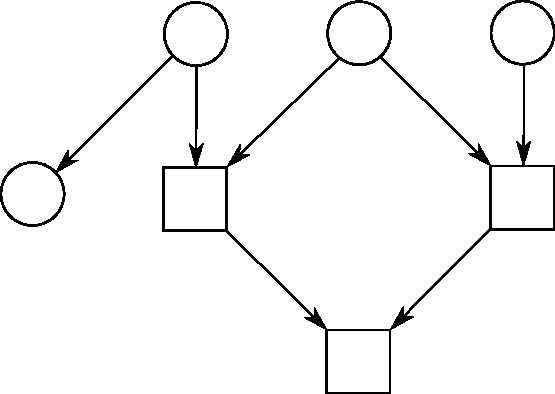
\includegraphics[width=\unitlength]{baysianmodel.pdf}}%
    \put(0.62968498,0.04171382){\color[rgb]{0,0,0}\makebox(0,0)[lb]{\smash{$S$}}}%
    \put(0.33638551,0.33553136){\color[rgb]{0,0,0}\makebox(0,0)[lb]{\smash{$F$}}}%
    \put(0.92239445,0.33553136){\color[rgb]{0,0,0}\makebox(0,0)[lb]{\smash{$C$}}}%
    \put(0.33586739,0.63038521){\color[rgb]{0,0,0}\makebox(0,0)[lb]{\smash{$X$}}}%
    \put(0.62968498,0.63149328){\color[rgb]{0,0,0}\makebox(0,0)[lb]{\smash{$U$}}}%
    \put(0.92671889,0.62934899){\color[rgb]{0,0,0}\makebox(0,0)[lb]{\smash{$T$}}}%
    \put(0.0420857,0.34096392){\color[rgb]{0,0,0}\makebox(0,0)[lb]{\smash{$Z$}}}%
  \end{picture}%
\endgroup%

\resizebox{1\textwidth}{!}{%% Creator: Inkscape inkscape 0.48.4, www.inkscape.org
%% PDF/EPS/PS + LaTeX output extension by Johan Engelen, 2010
%% Accompanies image file 'graphicalModel_temporal.pdf' (pdf, eps, ps)
%%
%% To include the image in your LaTeX document, write
%%   \input{<filename>.pdf_tex}
%%  instead of
%%   \includegraphics{<filename>.pdf}
%% To scale the image, write
%%   \def\svgwidth{<desired width>}
%%   \input{<filename>.pdf_tex}
%%  instead of
%%   \includegraphics[width=<desired width>]{<filename>.pdf}
%%
%% Images with a different path to the parent latex file can
%% be accessed with the `import' package (which may need to be
%% installed) using
%%   \usepackage{import}
%% in the preamble, and then including the image with
%%   \import{<path to file>}{<filename>.pdf_tex}
%% Alternatively, one can specify
%%   \graphicspath{{<path to file>/}}
%% 
%% For more information, please see info/svg-inkscape on CTAN:
%%   http://tug.ctan.org/tex-archive/info/svg-inkscape
%%
\begingroup%
  \makeatletter%
  \providecommand\color[2][]{%
    \errmessage{(Inkscape) Color is used for the text in Inkscape, but the package 'color.sty' is not loaded}%
    \renewcommand\color[2][]{}%
  }%
  \providecommand\transparent[1]{%
    \errmessage{(Inkscape) Transparency is used (non-zero) for the text in Inkscape, but the package 'transparent.sty' is not loaded}%
    \renewcommand\transparent[1]{}%
  }%
  \providecommand\rotatebox[2]{#2}%
  \ifx\svgwidth\undefined%
    \setlength{\unitlength}{514.815004bp}%
    \ifx\svgscale\undefined%
      \relax%
    \else%
      \setlength{\unitlength}{\unitlength * \real{\svgscale}}%
    \fi%
  \else%
    \setlength{\unitlength}{\svgwidth}%
  \fi%
  \global\let\svgwidth\undefined%
  \global\let\svgscale\undefined%
  \makeatother%
  \begin{picture}(1,0.36762093)%
    \put(0,0){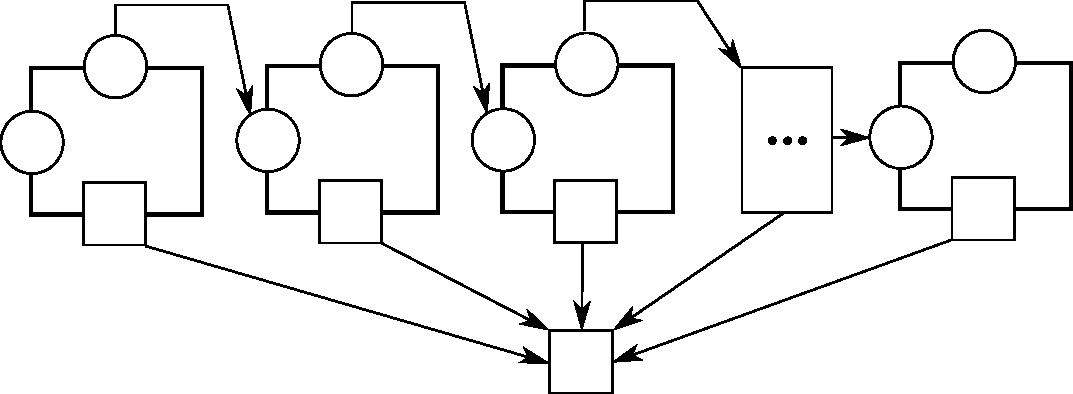
\includegraphics[width=\unitlength]{graphicalModel_temporal.pdf}}%
    \put(0.09547193,0.29665535){\color[rgb]{0,0,0}\makebox(0,0)[lb]{\smash{$U_0$}}}%
    \put(0.09407952,0.15956687){\color[rgb]{0,0,0}\makebox(0,0)[lb]{\smash{$S_0$}}}%
    \put(0.01881458,0.22563278){\color[rgb]{0,0,0}\makebox(0,0)[lb]{\smash{$Z_0$}}}%
    \put(0.31237857,0.29852096){\color[rgb]{0,0,0}\makebox(0,0)[lb]{\smash{$U_1$}}}%
    \put(0.31409408,0.16143247){\color[rgb]{0,0,0}\makebox(0,0)[lb]{\smash{$S_1$}}}%
    \put(0.23882916,0.22749837){\color[rgb]{0,0,0}\makebox(0,0)[lb]{\smash{$Z_1$}}}%
    \put(0.90558919,0.30139354){\color[rgb]{0,0,0}\makebox(0,0)[lb]{\smash{$U_n$}}}%
    \put(0.90419676,0.16430507){\color[rgb]{0,0,0}\makebox(0,0)[lb]{\smash{$S_n$}}}%
    \put(0.82893184,0.23037096){\color[rgb]{0,0,0}\makebox(0,0)[lb]{\smash{$Z_n$}}}%
    \put(0.53050271,0.02213156){\color[rgb]{0,0,0}\makebox(0,0)[lb]{\smash{$S_f$}}}%
    \put(0.53175169,0.29895161){\color[rgb]{0,0,0}\makebox(0,0)[lb]{\smash{$U_2$}}}%
    \put(0.53346717,0.16186314){\color[rgb]{0,0,0}\makebox(0,0)[lb]{\smash{$S_2$}}}%
    \put(0.4582022,0.22792902){\color[rgb]{0,0,0}\makebox(0,0)[lb]{\smash{$Z_2$}}}%
  \end{picture}%
\endgroup%
}
\captionsetup{justification=raggedright}
\caption{Chaining of the original graphical models.}
\label{fig:dbnet}
\end{figure}	
To describe the problem using a graphical model, we need to extend the above model in a temporal fashion. In Fig.~\ref{fig:boxmodel}, we first encapsulate the original graphical model into a block, where three variables are exposed to the outside. Then we chain the small blocks in series to obtain a new model as depicted in Fig.~\ref{fig:dbnet}. We use subscript $0,1,\cdots i$ to indicate the time dependency of the variables. The grasp process begins with the first measurement in time stamp zero. As a result, a dependency is created between $X_0$ and $Z_0$. Based on the sensing result, a control trajectory $U_0 = u_0$ is inferred to maximize the probability of success $S_0$. The robot performs one step of the trajectory $u_0$ and the grasping process moves on to the next time stamp. Since the camera also moves towards the object, the measurement at the next time stamp $Z_1$ depends on the last trajectory $U_0$ and the object state $X_1$. The sensing and control loop repeats until the last measurement $Z_i$ and control trajectory $U_i$ are taken. The conditional probability of success is formulated by 
\begin{equation}
 \pr(S_f=1| \underline{Z} = \underline{z},  \underline{U} = \underline{u}, \underline{T} = \underline{t}) = \frac{\sum\limits_{\substack{F_0,\cdots,F_n,\\ C_0,\cdots,C_n \\ X_0,\cdots X_n \\ S_0,\cdots S_n} }\pr( S = 1, \underline{F}, \underline{C}, \underline{X}, \underline{z},\underline{u}, \underline{t})} {P(\underline{Z} = \underline{z},  \underline{U} = \underline{u}, \underline{T} = \underline{t})} 
\label{equ:condition_prob_limit_sensing} 
\end{equation}
where $\underline{Z} = \{Z_0, \cdots, Z_n\}$, $ \underline{U} = \{U_0, \cdots, U_n\}$ and $\underline{C} = \{C_0, \cdots, C_n\}$. The condition $\underline{t} = \{t, \cdots, t\}$ indicates in each time stamp the task specifications are the same. Again, the nominator is computed by marginalizing the joint probability of all the variables  which are neither query nor conditions. The denominator is a renormalization constant. The joint probability distribution in the nominator can be computed based on the graph structure by 
\begin{equation}
\begin{split}
\pr( S_f = 1, \underline{F}, \underline{C}, \underline{X}, \underline{z},\underline{u},\underline{t}) = \prod\limits_{i = 1:n} &\pr(F_i | X_i, u_i) \cdot \pr(C_i | u_i, t)\cdot   \pr(z_i|u_{i-1}, X_i) \\
              \cdot & \pr(F_0 | X_0, u_0)\cdot \pr(C_0 | u_0, t)  \pr(z_0|X_0 )\\
              \cdot &\pr(S_i | F_i, C_i) \cdot  \pr(S_f=1| S_1, \cdots, S_n)   \\
              \cdot &\pr(X_i)\cdot P(u_i) \cdot\pr(X_0) \cdot \pr(u_0) 
\end{split}
\label{equ:cpd_graph}
\end{equation}
First, we eliminate discrete variables $\underline{F}$, $\underline{C}$ and $\underline{S}$.
The term $\pr(S_f=1| S_1, \cdots, S_n)$ equals zero as long as one of the $S_i$ does not equal to one. Therefore, after marginalization of $\underline{S}$ the nominator equals
\begin{equation}
\begin{split}
\sum\limits_{\substack{F_0,\cdots,F_n,\\ C_0,\cdots,C_n \\ X_0,\cdots X_n \\ S_0,\cdots S_n} }\pr( S_f = 1, \underline{F}, \underline{C}, \underline{X}, \underline{z},\underline{u}, \underline{t}) = \sum\limits_{\substack{F_0,\cdots,F_n,\\ C_0,\cdots,C_n \\ X_0,\cdots X_n  }} \pr( S_f = 1, \underline{S} = \underline{1}, \underline{F}, \underline{C}, \underline{X}, \underline{z},\underline{u}, \underline{t})
\end{split}
\label{equ:after_maginalizing_s}
\end{equation}
The same principle also applies to $F_i$ and $C_i$, because the term $\pr(S_i = 1 | F_i, C_i)$ equals zero everywhere except at $F_i=1,C_i=1 $. After we eliminate all the  $F_i$ and $C_i$, the nominator of equation \ref{equ:condition_prob_limit_sensing} equals to 
\begin{equation}
\begin{split}
\sum\limits_{\substack{F_0,\cdots,F_n,\\ C_0,\cdots,C_n \\ X_0,\cdots X_n \\ S_0,\cdots S_n} }\pr( S_f = 1, \underline{F}, \underline{C}, \underline{X}, \underline{z},\underline{u}, \underline{t}) = \sum\limits_{ X_0,\cdots X_n } \pr( S_f = 1, \underline{S} = \underline{1}, \underline{F} = \underline{1}, \underline{C} = \underline{1}, \underline{X}, \underline{z},\underline{u}, \underline{t})
\end{split}
\label{equ:after_maginalizing_cf}
\end{equation}
Substituting the term after sum operation by \ref{equ:cpd_graph}, we obtain 
\begin{equation}
\begin{split}
 &\sum\limits_{ X_0,\cdots X_n } \pr( S_f = 1, \underline{S} = \underline{1}, \underline{F} = \underline{1}, \underline{C} = \underline{1}, \underline{X}, \underline{z},\underline{u}, \underline{t}) \\
=&\sum\limits_{ X_0,\cdots X_n } \prod\limits_{i = 1:n} \pr(F_i=1 | X_i, u_i) \cdot \pr(C_i = 1 | u_i, t)\cdot   \pr(z_i|u_{i-1}, X_i) \\
              \cdot & \pr(F_0=1 | X_0, u_0)\cdot \pr(C_0=1 | u_0, t)  \pr(z_0|X_0 )\\
              \cdot & \underbrace{\pr(S_i = 1 | F_i = 1, C_i=1)}_{=1} \cdot  \underbrace{\pr(S_f=1| S_1, \cdots, S_n = 1)}_{=1}  \\
              \cdot &\pr(X_i)\cdot P(u_i) \cdot\pr(X_0) \cdot \pr(u_0) \\
=&  \prod\limits_{i = 1:n} \underbrace{   \sum\limits_{ X_i} \pr(F_i=1 | X_i, u_i) \cdot \pr(C_i = 1 | u_i, t)\cdot   \pr(z_i|u_{i-1}, X_i) \cdot \pr(X_i) }_{\phi_i(u_i, u_{i-1}) } \\ 
  & \cdot \underbrace{ \sum\limits_{ X_0} \pr(F_0 =1 | X_0, u_0)\cdot \pr(C_0=1 | u_0, t)  \pr(z_0|X_0 ) \cdot \pr(X_0) }_{\phi_0(u_0)} \\ 
  &  \cdot \underbrace{ \pr(u_i) \cdot \pr(u_0) }_{\text{constant}} \\
  \propto &  \prod\limits_{i = 1:n} \phi_i(u_i, u_{i-1}) \cdot \phi_0(u_0).
\end{split}
\end{equation}

Incorporating the renormalization constant in the denominator of Equ.~\ref{equ:condition_prob_limit_sensing}, the conditional probability of grasping success is proportional to the multiplication of a set of factors $\phi_i$.    
\begin{equation}
\begin{split}
&  \pr(S_f=1| \underline{Z} = \underline{z},  \underline{U} = \underline{u}, \underline{T} = \underline{t}) \\
\propto & \prod\limits_{i = 1:n} \phi_i(u_i, u_{i-1}) \cdot \phi_0(u_0).
\end{split}
\end{equation}
As same as in the previous grasping scenario, we aim to find $u_0^*$ to $u_n^*$ to maximize the conditional probability. However, due to the temporal property of the model, we can not condition all the measurements $\underline{Z}$ at once. The conditioning of the measurement depends on what control trajectory $u$ is sent to the robot at the last time stamp. Therefore, the optimal control sequence  $u_0^*:u_t^*$ can only be found in an iterative fashion. We propose to use the following paradigm to find optimal controls for the robot. 
\begin{algorithm}[!htbp]
\begin{algorithmic}[1]
\STATE $u_0^*  = \argmax\limits_{u_0}  \phi_0(u_0)   $
\STATE execute $u_0^*$ on robot 
\STATE wait for a time step
\FOR {$i$ from 1 to $n$}
\STATE $u_i^*  = \argmax\limits_{u_i}  \phi_i(u_i ,u_{i-1}^* ) $ 
\STATE execute $u_i^*$ on robot 
\STATE wait for a time step 
\IF {pre-touch configuration is reached}
\RETURN success
\ENDIF
\ENDFOR 
%\captionsetup{justification=raggedright}
\caption {Paradigm for iteratively finding optimal control trajectory}
\label{paradigmforgrasping}
\end{algorithmic}
\end{algorithm}

 \section{Summary}
 In this chapter, we first propose a unified model based on Bayesian networks to describe grasping problems. The network we define for the grasping problem factorizes the joint distribution into smaller conditional probability distributions. By conditioning on a subset of variables such as measurement and robot controls, we can compute the conditional probability of success. The goal is to determine the controls that maximize the conditional probability of success. Then we derive how to compute the conditional success probability in three different grasping scenarios. The focus of each scenario is different. In the first scenario, we consider grasping known objects under task constraint. As the object is known to the robot, force closure and representation of the object are not an issue. The focus in this scenario is how to model the task constraint satisfaction. In the second scenario, we consider the problem of grasping unknown objects. The focus is how to model the probability of force closure and how to model the object. In the third scenario, we consider the problem that the robot only has limited sensing capability. To reduce perception uncertainty, the model is extended in a temporal fashion to allow continuous measurement integration. The focus is how to find optimal controls online in each iteration. In the following chapters, we will elaborate how the grasping problem is solved in each grasping scenarios.




 

\cleardoublepage
\thispagestyle{empty}
\chapter{Design of Grasp Strategies for Mobile Manipulation Systems}
\section{Introduction}

\section{Related Work}

\section{Strategies generation for pre-grasp phase}

\subsection{Active perception for unknown object surfaces}

\subsection{Active interaction for quasi-static objects }	


\section{Exploit the mobility to perform the planed strategies}

\subsection{Reachability analysis with given environment models}

\subsection{Base position planning}


\subsection{Arm-Base coordination}


\cleardoublepage
\thispagestyle{empty}
\chapter{A Probabilistic Approach to Grasp Synthesis}

\section{Introduction}

\section{Related work}

\section{Contributions}

\section{Probabilistic modelling of grasping success}
Grasp motion, is the key phase
in the entire grasping process. During this phase, the robot has to estimate the object pose and geometry, predict the likelihood of success with a pre-touch configuration and choose the action that maximizes the
grasping success probability. This sections gives the mathematic model of grasping success, followed by a the proof of the model with an 1-D grasping example. 
\subsection{Mathematic Model}
First we define a random variable $S \in \{ \text{success} , \text{failure} \}$ as the outcome of a specific grasp motion $\mathcal{G} = \{g_1, \dots ,g_n$\}, with $g_1, \dots ,g_n$ representing a set of gripper configurations and poses. We define $\text{P}({S = \text{success}}|\mathcal{G},\mathcal{Z})$ as the marginal probability that the grasp $\mathcal{G}$ succeeds based on the sensor measurement history $\mathcal{Z}=\lbrace z_0, \dots ,z_M \rbrace$. It is not straightforward to compute the marginal probability $\text{P}({S = \text{success}}|\mathcal{G},\mathcal{Z})$ directly without knowing the state of the object 
$x_o$. However, we can compute it by separating it into two probability terms: 
\begin{equation}
\text{P}(S) := \text{P}(S | \mathcal{G} ,\mathcal{Z}) = \int_{x_o} \text{P} (S | x_o,\mathcal{G} )\cdot p(x_o|\mathcal{Z}) dx_o. 
\label{e_grasp_success}
\end{equation}
We call the first term $P(S | x_o,\mathcal{G})$ conditional grasping success model. It indicates how likely a specific grasping action $\mathcal{G}$ will lead to a success given the object state $x_o$. The second term $p(x_o|\mathcal{Z})$ represents the posterior probability of the object given a series of observations, which quantifies the perception uncertainty. In this way, the problem of predicting the marginal grasp success probability is simplified to model the $P(S | x_o,\mathcal{G})$, and to model the perception uncertainty. 

After the marginal grasp probability $\text{P}(S)$ is computed, the next step is to find an optimal grasping motion $\mathcal{G}_\text{opt}$ that maximizes the marginal grasp success probability:
\begin{equation}
\mathcal{G}_\text{opt} = \argmax_\mathcal{G} \text{P}(S).
\label{eq_g_opt}
\end{equation}

\subsection{Verification of the concept}
To verify the proposed mathematic model, we apply this formulation to solve an 1-D grasping problem. We aim to compute the optimal pre-touch configuration for a simple parallel gripper to grasp an 1-D rigid  object with width $w$. $x$ defines the position of the object. The parallel gripper has a limited opening width constrained by $u_1 \in [0, u_{1}^{\text{max}}]$. $u_2$ defines the position of the gripper. We assume that the grasp motion $\mathcal{G}$ only contains one gripper configuration defined by $\{ (u_1,u_2) \}$. Fig.~\ref{fig:1D_simple} depicts this 1-D grasping example.

\begin{figure}[!htbp]
\centering
\def\svgwidth{0.8\linewidth}
%% Creator: Inkscape inkscape 0.48.4, www.inkscape.org
%% PDF/EPS/PS + LaTeX output extension by Johan Engelen, 2010
%% Accompanies image file '1dillustration.pdf' (pdf, eps, ps)
%%
%% To include the image in your LaTeX document, write
%%   \input{<filename>.pdf_tex}
%%  instead of
%%   \includegraphics{<filename>.pdf}
%% To scale the image, write
%%   \def\svgwidth{<desired width>}
%%   \input{<filename>.pdf_tex}
%%  instead of
%%   \includegraphics[width=<desired width>]{<filename>.pdf}
%%
%% Images with a different path to the parent latex file can
%% be accessed with the `import' package (which may need to be
%% installed) using
%%   \usepackage{import}
%% in the preamble, and then including the image with
%%   \import{<path to file>}{<filename>.pdf_tex}
%% Alternatively, one can specify
%%   \graphicspath{{<path to file>/}}
%% 
%% For more information, please see info/svg-inkscape on CTAN:
%%   http://tug.ctan.org/tex-archive/info/svg-inkscape
%%
\begingroup%
  \makeatletter%
  \providecommand\color[2][]{%
    \errmessage{(Inkscape) Color is used for the text in Inkscape, but the package 'color.sty' is not loaded}%
    \renewcommand\color[2][]{}%
  }%
  \providecommand\transparent[1]{%
    \errmessage{(Inkscape) Transparency is used (non-zero) for the text in Inkscape, but the package 'transparent.sty' is not loaded}%
    \renewcommand\transparent[1]{}%
  }%
  \providecommand\rotatebox[2]{#2}%
  \ifx\svgwidth\undefined%
    \setlength{\unitlength}{244.80062425bp}%
    \ifx\svgscale\undefined%
      \relax%
    \else%
      \setlength{\unitlength}{\unitlength * \real{\svgscale}}%
    \fi%
  \else%
    \setlength{\unitlength}{\svgwidth}%
  \fi%
  \global\let\svgwidth\undefined%
  \global\let\svgscale\undefined%
  \makeatother%
  \begin{picture}(1,0.30919334)%
    \put(0,0){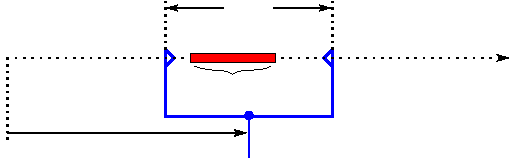
\includegraphics[width=\unitlength]{1dillustration.pdf}}%
    \put(0.15949338,0.01813248){\color[rgb]{0,0,0}\makebox(0,0)[lb]{\smash{$u_2$}}}%
    \put(0.40692504,0.22646518){\color[rgb]{0,0,0}\makebox(0,0)[lb]{\smash{object}}}%
    \put(0.96767264,0.21229788){\color[rgb]{0,0,0}\makebox(0,0)[lb]{\smash{$x$}}}%
    \put(0.44163201,0.13862415){\color[rgb]{0,0,0}\makebox(0,0)[lb]{\smash{$w$}}}%
    \put(0.4455571,0.29089082){\color[rgb]{0,0,0}\makebox(0,0)[lb]{\smash{$u_1$}}}%
    \put(-0.00215418,0.21245965){\color[rgb]{0,0,0}\makebox(0,0)[lb]{\smash{0}}}%
  \end{picture}%
\endgroup%

\captionsetup{justification=raggedright}
\caption{Illustration of an 1-D grasping problem.}
\label{fig:1D_simple}
\end{figure}	

First let us  derive a grasp success probability model $\text{P}(S | x,  \mathcal{G} )$ for this example. Since the positions of the finger tips can determine whether a gripper configuration will succeed, we can compute these positions directly from $u_1$ and $u_2$ by   

%It is obviously that when the  position of the gripper is equal to the position of the object ($u_2 = x$) and the opening width of the gripper is equal to the width of the object ($u_1 = w$), a stable grasp is then established. We define this configuration as a reference $u^{\text{ref}}$: 
%\begin{equation}
%u^{\text{ref}} =  \begin{pmatrix}\begin{figure}
%u_1^{\text{ref}}\\ 
%u_2^{\text{ref}}
%\end{pmatrix}
%=\begin{pmatrix}
%w\\ 
%x
%\end{pmatrix}. 
%\end{equation}
%and assign the probability of grasp success of this configuration with $\text{P}(S | x = x_0, \mathcal{G} = u^{\text{ref}}) = 1$.
\begin{equation}
\begin{pmatrix}
c^{\text{left}}\\ 
c^{\text{right}}
\end{pmatrix}
=\begin{pmatrix}
u_2 - 0.5 \cdot u_1\\ 
u_2 + 0.5 \cdot u_1
\end{pmatrix}.
\end{equation}
If the finger tips are in intersect with the object, the grasp is invalid. In these cases, we assign the probability of grasp success to zero. When the positions of finger tips fullfill the condition ( $c^{\text{left}} < x - 0.5w$ and $c^{\text{right}} > x + 0.5w$ ), the object can be grasped by the gripper. However, for precision grasping, we want to avoid object displacement during grasping. During the phase of force closure, we want the object to move as little as possible. Therefore, a term that penalizes object displacement can be introduced into the grasp success model. We model the grasp success probability by 

\begin{equation}
  \text{P}(S | x,  \mathcal{G} )  = -\frac{1}{ d^{\text{max}} } \cdot d + 1,
  \label{equ:5}
\end{equation}
where $d^{\text{max}}  = 0.5 \cdot (u_{1}^{\text{max}} - w) $ denotes the maximum displacement that can be executed by a gripper. $d = | u_2 - x | $ denotes the actual object displacement. By combining this model with a given object posterior $p(x|\mathcal{Z})$, a marginal success probability $\text{P}(S)$ can be obtained by evaluating Eq.~\ref{e_grasp_success}. To illustrate how an object posterior can influence marginal success probability, we choose object length $w = 0.2$, the maximal opening width of the gripper $u_{1}^{\text{max}} = 0.4 $. We compare the result by using two different object posteriors to simulate an accurate and a less accurate perception system. We model the $p(x|\mathcal{Z})$ by two Gaussian distributions with $\mathcal{N}(0, 0.3)$ and $\mathcal{N}(0, 0.03)$ respectively. Fig.~\ref{fig:1D_grasp} depicts the contour of grasp success probability $\text{P}(S)$ in terms of the pre-touch configuration.

\begin{figure}[!htbp]
\centering
\def\svgwidth{1\linewidth}
%% Creator: Inkscape inkscape 0.48.4, www.inkscape.org
%% PDF/EPS/PS + LaTeX output extension by Johan Engelen, 2010
%% Accompanies image file '1dgrasp_result.pdf' (pdf, eps, ps)
%%
%% To include the image in your LaTeX document, write
%%   \input{<filename>.pdf_tex}
%%  instead of
%%   \includegraphics{<filename>.pdf}
%% To scale the image, write
%%   \def\svgwidth{<desired width>}
%%   \input{<filename>.pdf_tex}
%%  instead of
%%   \includegraphics[width=<desired width>]{<filename>.pdf}
%%
%% Images with a different path to the parent latex file can
%% be accessed with the `import' package (which may need to be
%% installed) using
%%   \usepackage{import}
%% in the preamble, and then including the image with
%%   \import{<path to file>}{<filename>.pdf_tex}
%% Alternatively, one can specify
%%   \graphicspath{{<path to file>/}}
%% 
%% For more information, please see info/svg-inkscape on CTAN:
%%   http://tug.ctan.org/tex-archive/info/svg-inkscape
%%
\begingroup%
  \makeatletter%
  \providecommand\color[2][]{%
    \errmessage{(Inkscape) Color is used for the text in Inkscape, but the package 'color.sty' is not loaded}%
    \renewcommand\color[2][]{}%
  }%
  \providecommand\transparent[1]{%
    \errmessage{(Inkscape) Transparency is used (non-zero) for the text in Inkscape, but the package 'transparent.sty' is not loaded}%
    \renewcommand\transparent[1]{}%
  }%
  \providecommand\rotatebox[2]{#2}%
  \ifx\svgwidth\undefined%
    \setlength{\unitlength}{259.88395945bp}%
    \ifx\svgscale\undefined%
      \relax%
    \else%
      \setlength{\unitlength}{\unitlength * \real{\svgscale}}%
    \fi%
  \else%
    \setlength{\unitlength}{\svgwidth}%
  \fi%
  \global\let\svgwidth\undefined%
  \global\let\svgscale\undefined%
  \makeatother%
  \begin{picture}(1,0.53724423)%
    \put(0,0){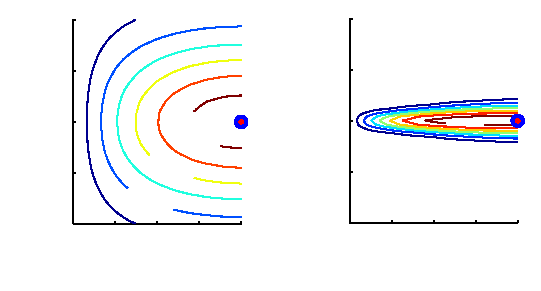
\includegraphics[width=\unitlength]{1dgrasp_result.pdf}}%
    \put(0.1151589,0.08992018){\makebox(0,0)[lb]{\smash{0.2}}}%
    \put(0.18217497,0.08992018){\makebox(0,0)[lb]{\smash{0.25}}}%
    \put(0.27003572,0.08992018){\makebox(0,0)[lb]{\smash{0.3}}}%
    \put(0.33673164,0.08992018){\makebox(0,0)[lb]{\smash{0.35}}}%
    \put(0.4249133,0.08992018){\makebox(0,0)[lb]{\smash{0.4}}}%
    \put(0.08972926,0.1171398){\makebox(0,0)[lb]{\smash{-0.5}}}%
    \put(0.07593948,0.20747584){\color[rgb]{0,0,0}\makebox(0,0)[lb]{\smash{-0.25}}}%
    \put(0.10355064,0.2982193){\makebox(0,0)[lb]{\smash{0}}}%
    \put(0.08669901,0.39782419){\makebox(0,0)[lb]{\smash{0.25}}}%
    \put(0.09666237,0.48644253){\makebox(0,0)[lb]{\smash{0.5}}}%
    \put(0.23790599,0.1699559){\rotatebox{-22.99998994}{\makebox(0,0)[lb]{\smash{0.04}}}}%
    \put(0.27574288,0.23088155){\rotatebox{-25.9999936}{\makebox(0,0)[lb]{\smash{0.08}}}}%
    \put(0.33923275,0.31457275){\rotatebox{-51.0000188}{\makebox(0,0)[lb]{\smash{0.12}}}}%
    \put(0.01695468,0.30375214){\color[rgb]{0,0,0}\makebox(0,0)[lb]{\smash{$u_2$}}}%
    \put(0.27728722,0.04517519){\color[rgb]{0,0,0}\makebox(0,0)[lb]{\smash{$u_1$}}}%
    \put(0.61970258,0.09198088){\makebox(0,0)[lb]{\smash{0.2}}}%
    \put(0.68671864,0.09198088){\makebox(0,0)[lb]{\smash{0.25}}}%
    \put(0.77457939,0.09198088){\makebox(0,0)[lb]{\smash{0.3}}}%
    \put(0.84127531,0.09198088){\makebox(0,0)[lb]{\smash{0.35}}}%
    \put(0.92945698,0.09198088){\makebox(0,0)[lb]{\smash{0.4}}}%
    \put(0.83165564,0.29547016){\rotatebox{-3.00000411}{\makebox(0,0)[lb]{\smash{0.7}}}}%
    \put(0.52418668,0.30637183){\color[rgb]{0,0,0}\makebox(0,0)[lb]{\smash{$u_2$}}}%
    \put(0.7845194,0.05087321){\color[rgb]{0,0,0}\makebox(0,0)[lb]{\smash{$u_1$}}}%
    \put(0.26204153,0.00490434){\color[rgb]{0,0,0}\makebox(0,0)[lb]{\smash{(a)}}}%
    \put(0.79104124,0.0040583){\color[rgb]{0,0,0}\makebox(0,0)[lb]{\smash{(b)}}}%
    \put(0.58730417,0.21390265){\color[rgb]{0,0,0}\makebox(0,0)[lb]{\smash{-0.25}}}%
    \put(0.59889533,0.11916901){\makebox(0,0)[lb]{\smash{-0.5}}}%
    \put(0.61271672,0.30024851){\makebox(0,0)[lb]{\smash{0}}}%
    \put(0.59586509,0.3998534){\makebox(0,0)[lb]{\smash{0.25}}}%
    \put(0.60582844,0.48847175){\makebox(0,0)[lb]{\smash{0.5}}}%
  \end{picture}%
\endgroup%

\caption{ Marginal grasp success probability in terms of two different object posteriors. The optimal gripper configurations are shown by red dots. In (a), $\mathcal{N}(0, 0.3)$ is used to simulate the posterior of the object position. The marginal success probability ${\text{P}(S)}_{u = u_{\text{opt}}} = 0.13$  . In (b) $\mathcal{N}(0, 0.03)$ is used to simulate a more accurate posterior distribution of the object position with ${\text{P}(S)}_{u = u_{\text{opt}}} = 0.76$ }
\label{fig:1D_grasp}
\end{figure}	 


\subsection{Modelling of conditional grasp success probability }
For real world objects, it is required to have a conditional grasp success model that consider much more factors than the 1-D example, so that the conditional grasp success model can approximate the true probability. Two conditions are necessary to ensure a successful grasp. First, the motion of a gripper, which is represented by $\mathcal{G}$, should not collide with the environment and the object. Second, the last pose and posture $g_n$ which we define as the pre-touch configuration should guarantee that forces from the finger tips are established on the object in the third phase. For the first condition we assume that there is sufficient free space between the pre-grasp configuration and the pre-touch configuration. The collision-free motion from the pre-grasp to the pre-touch can be computed using a pre-defined heuristic: approaching with a linear motion. To fullfill the second condition, the choice of a pre-touch configuration $g_n$ is essential, because the grasp success is predominantly affected by the way we make contact with the object. Hence, the grasp success model $P(S | x,\mathcal{G})$ is simplified to $P(S | x, g_n$). 

The dimension of the object state $x$ depends on the choice of an object representation. To represent simple geometry primitives such as cylindrical objects, it is sufficient to choose a parametric representation which includes radius, height, and the position of the object. For objects which form are irregular, the dimension of $x$ can be very large. However, predicting the grasp success probability can be independent of the choice of representation, since it is only required to extract the contact normals of an object.  

In the following we elaborate on how we calculate the conditional success probability of a pre-touch configuration $g_n$ for real world objects. Here we only study the pinch grasp, that a grasp only requires two fingers to make contact with the object. Pinch grasp can be easily realized by most grippers, independent of how many fingers a gripper having. We choose three criteria to model the conditional grasp success probability. 

\begin{figure}[!htbp]
\centering
\def\svgwidth{0.7\linewidth}
%% Creator: Inkscape inkscape 0.48.4, www.inkscape.org
%% PDF/EPS/PS + LaTeX output extension by Johan Engelen, 2010
%% Accompanies image file 'bunny.pdf' (pdf, eps, ps)
%%
%% To include the image in your LaTeX document, write
%%   \input{<filename>.pdf_tex}
%%  instead of
%%   \includegraphics{<filename>.pdf}
%% To scale the image, write
%%   \def\svgwidth{<desired width>}
%%   \input{<filename>.pdf_tex}
%%  instead of
%%   \includegraphics[width=<desired width>]{<filename>.pdf}
%%
%% Images with a different path to the parent latex file can
%% be accessed with the `import' package (which may need to be
%% installed) using
%%   \usepackage{import}
%% in the preamble, and then including the image with
%%   \import{<path to file>}{<filename>.pdf_tex}
%% Alternatively, one can specify
%%   \graphicspath{{<path to file>/}}
%% 
%% For more information, please see info/svg-inkscape on CTAN:
%%   http://tug.ctan.org/tex-archive/info/svg-inkscape
%%
\begingroup%
  \makeatletter%
  \providecommand\color[2][]{%
    \errmessage{(Inkscape) Color is used for the text in Inkscape, but the package 'color.sty' is not loaded}%
    \renewcommand\color[2][]{}%
  }%
  \providecommand\transparent[1]{%
    \errmessage{(Inkscape) Transparency is used (non-zero) for the text in Inkscape, but the package 'transparent.sty' is not loaded}%
    \renewcommand\transparent[1]{}%
  }%
  \providecommand\rotatebox[2]{#2}%
  \ifx\svgwidth\undefined%
    \setlength{\unitlength}{194bp}%
    \ifx\svgscale\undefined%
      \relax%
    \else%
      \setlength{\unitlength}{\unitlength * \real{\svgscale}}%
    \fi%
  \else%
    \setlength{\unitlength}{\svgwidth}%
  \fi%
  \global\let\svgwidth\undefined%
  \global\let\svgscale\undefined%
  \makeatother%
  \begin{picture}(1,0.67409794)%
    \put(0,0){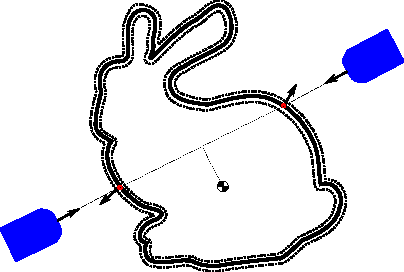
\includegraphics[width=\unitlength]{bunny.pdf}}%
    \put(0.12693299,0.16410315){\color[rgb]{0,0,0}\makebox(0,0)[lb]{\smash{$n_1$}}}%
    \put(0.7863913,0.49764194){\color[rgb]{0,0,0}\makebox(0,0)[lb]{\smash{$n_2$}}}%
    \put(0.64071158,0.3573397){\color[rgb]{0,0,0}\makebox(0,0)[lb]{\smash{$c_2$}}}%
    \put(0.31678681,0.21094795){\color[rgb]{0,0,0}\makebox(0,0)[lb]{\smash{$c_1$}}}%
    \put(0.19497423,0.18987635){\color[rgb]{0,0,0}\makebox(0,0)[lb]{\smash{$d_1$}}}%
    \put(0.76565879,0.40945617){\color[rgb]{0,0,0}\makebox(0,0)[lb]{\smash{$d_2$}}}%
  \end{picture}%
\endgroup%

\caption{Description of variables which represent a pre-touch configuration $g_n$ on an bunny object. Fingertips are illustrated in blue. Dashed lines indicate variances of the representation. Arrows represent normals on the particular surfaces.}
\label{fig:grasp_generation}
\end{figure}

\begin{itemize}
\item \textit{Non-zero contact angle}: 
 The first criterion that affects the grasp success is the angle between normal of finger tips and desired contact regions. In Fig.~\ref{fig:grasp_generation}, we denote $n_i$ as the normal defined on a finger tip and $c_i$ as the normal of a contact region. $d_i$ is the distance from a finger tip to a contact region. The grasp success probability with a non-zero contact angle is given by:
\begin{equation}
P_1 = \begin{cases}
\prod_{i=1}^{k}(-\frac{1}{0.5\cdot \theta} |\beta|) + 1 )  & |\beta | < \frac{\theta}{2}\\
  0   & \text{else}
\end{cases},
\end{equation} 
where $\beta = \pi - \angle(n_i,c_i)$ and $\angle(n_i,c_i)$ is the angle between $n_i$ and $c_i$.  $k$ denotes the total number of finger tips used to make contact with the object. $\theta$ is the maximal angle of a friction cone that the finger tip still supports the object without slipping. 
\item \textit{Non-optimal finger placement}:
Due to the non-optimal control of a gripper during force closure, the closer the finger tips are located to the object surface, the less likely a control error would occur to influence the overall grasp success. Therefore this criterion is modelled by 
\begin{equation} 
P_2 = \text{exp}\left(-\sum_{i=1}^k \frac{d_i-h}{\sigma_h^2}\right)
\end{equation}
where $h$ is the desired offset distance between finger tips and the object's surface for a pre-touch configuration. $\sigma_h$ is a shaping factor for the probability. 

\todo {\item \textit{Distance to center of gravity}:}
 

\item \textit{Surface uncertainty}:
 This criterion is specially designed for the representation that is able to model surface uncertainty. This criterion avoids to make finger contacts on uncertain surfaces, because contacts established on uncertain surfaces can not guarantee firm contacts between the finger tips and the object. We model the success probability of uncertain contacts induced by surface uncertainty with 
\begin{equation}
 P_3 =  \begin{cases}
\prod_{i=1}^{k}(-\frac{1}{\sigma_{\text{max}} } \mean{\sigma(c_i)}  + 1 )  &  \mean{\sigma(c_i)} < \sigma_{\text{max}}\\
  0   & \text{else}
\end{cases},
\end{equation} 
where $\mean{\sigma(c_i)} $ is an average variance of $c_i$ and $\sigma_{\text{max}}$ is a parameter representing the maximal allowed variance. We merge the proposed  criteria in a weighted fashion to generate an overall grasp success probability by  
\begin{equation}
P(S | x , g_n) =  \sum_{i=1}^3 w_i \cdot P_i
\end{equation} 
with $\sum_{i=1}^3 w_i  = 1$.
\end{itemize}

\subsection{Model validation}
We choose a 2-D grasp scenario to validate the model of  conditional grasp success probability. A circular object is chosen as the target object. The circular object is represented by three parameters: radius $\in \mathcal{R}$ and position $\in \mathcal{R}^2$. A parallel gripper is chose to grasp the object. The gripper configuration $\in \mathcal{R}^4$ contains the 2D positions of the left finger and the right finger. We simplify the grasp trajectory $\mathcal{G}$ to $g_n$, which is by definition the pre-touch configuration.  A number of random gripper pre-touch configurations is generated. For each configuration we evaluate the conditional grasp success probability. Fig.~\ref{fig:circular_grasp_success}(a) depicts 10 random gripper configurations, the grasp success probability of which are higher than 90~$\%$. Fig.~\ref{fig:circular_grasp_success}(b) shows 10 negative examples, the conditional grasp success probability of which are lower than 10~$\%$. 

The optimal pre-touch configuration is found according to equation \ref{eq_g_opt} by searching the maximal marginal grasp probability. Since the dimension of object state for a circular object is only three, we can integrate the equation \ref{e_grasp_success} numerically. Suppose the posterior of the object state can be represented by a multi-variate Gaussian $p(x_o|\mathcal{Z}) = \mathcal{N}(\mu, \Sigma)$ where $\mu$ is a mean and $\Sigma$ is a covariance matrix. The integral of equation  \ref{e_grasp_success} can be approximated by 

\begin{equation}
\begin{split}
 \text{P}(S | \mathcal{G} ,\mathcal{Z}) &= \text{P}(S | g_n ,\mathcal{Z}) \\
    &= \int_{x_o} \text{P} (S | x_o, g_n )\cdot p(x_o|\mathcal{Z}) dx_o \\
    &=  \int_{x_o} \text{P} (S | x_o, g_n )\cdot \mathcal{N}(\mu, \Sigma) dx_o  \\
    &\approx \int_{\mu_1 - \sigma_1}^{\mu_1 + \sigma_1} \int_{\mu_2 - \sigma_2}^{\mu_2 + \sigma_2} \int_{\mu_3 - \sigma_3}^{\mu_3 + \sigma_3} \text{P} (S | x_{o},  g_n )\cdot \mathcal{N}(\mu, \Sigma)  dx_{1} dx_{2} dx_{3}, 
\label{e_grasp_success}
\end{split}
\end{equation}
where $x_{1}, x_{2}, x_{3} $ represent the radius and the positions, $\mu_1, \mu_2, \mu_3$ are the means of positions and the radius. $\sigma_1, \sigma_2, \sigma_3$ are the diagonal elements of the covariance matrix $\Sigma$. In this case, we use Subplex \todo{[cite]\cite{}}(a variant of Nelder-Mead for function minimization) implemented in NLopt \todo{[cite]\cite{}} to find the maximal probability of $\text{P}(S | g_n ,\mathcal{Z})$. Fig.~\ref{fig:object_posterior_sample} visualizes a synthetic posterior distribution   with $\mu = (0, 0 , 0.01)$ and $
\Sigma = 
\begin{pmatrix}
0.01 & 0.008  & 0 \\ 
0.008 & 0.01  & 0 \\
0 & 0  & 0.01
\end{pmatrix}
$. The optimal pre-touch configuration for this posterior is depicted in Fig.~\ref{fig:optimal_pre_touch_conf}. The marginal success probability of this object posterior by taking the optimal pre-touch configuration is equal to $44.9 \%$. The absolute mass of probability depends on how the parameters are chosen for evaluating the conditional success grasp probability. Since the parameters we choose for calculating the conditional success grasp probability for this example is conservative, the success probability by taking the optimal pre-touch configuration is not high. However, the pre-touch configurations computed using our model are very close to the optimal in reality. From the figure we can see, that the grasp is explicitly computed for the given object state uncertainty. 

\begin{figure}[!htbp]
\centering
\def\svgwidth{1\linewidth}
%% Creator: Inkscape inkscape 0.48.4, www.inkscape.org
%% PDF/EPS/PS + LaTeX output extension by Johan Engelen, 2010
%% Accompanies image file 'grasp_success_circular.pdf' (pdf, eps, ps)
%%
%% To include the image in your LaTeX document, write
%%   \input{<filename>.pdf_tex}
%%  instead of
%%   \includegraphics{<filename>.pdf}
%% To scale the image, write
%%   \def\svgwidth{<desired width>}
%%   \input{<filename>.pdf_tex}
%%  instead of
%%   \includegraphics[width=<desired width>]{<filename>.pdf}
%%
%% Images with a different path to the parent latex file can
%% be accessed with the `import' package (which may need to be
%% installed) using
%%   \usepackage{import}
%% in the preamble, and then including the image with
%%   \import{<path to file>}{<filename>.pdf_tex}
%% Alternatively, one can specify
%%   \graphicspath{{<path to file>/}}
%% 
%% For more information, please see info/svg-inkscape on CTAN:
%%   http://tug.ctan.org/tex-archive/info/svg-inkscape
%%
\begingroup%
  \makeatletter%
  \providecommand\color[2][]{%
    \errmessage{(Inkscape) Color is used for the text in Inkscape, but the package 'color.sty' is not loaded}%
    \renewcommand\color[2][]{}%
  }%
  \providecommand\transparent[1]{%
    \errmessage{(Inkscape) Transparency is used (non-zero) for the text in Inkscape, but the package 'transparent.sty' is not loaded}%
    \renewcommand\transparent[1]{}%
  }%
  \providecommand\rotatebox[2]{#2}%
  \ifx\svgwidth\undefined%
    \setlength{\unitlength}{201.33696562bp}%
    \ifx\svgscale\undefined%
      \relax%
    \else%
      \setlength{\unitlength}{\unitlength * \real{\svgscale}}%
    \fi%
  \else%
    \setlength{\unitlength}{\svgwidth}%
  \fi%
  \global\let\svgwidth\undefined%
  \global\let\svgscale\undefined%
  \makeatother%
  \begin{picture}(1,0.49955409)%
    \put(0,0){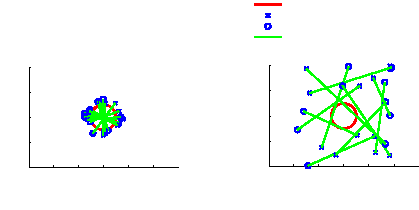
\includegraphics[width=\unitlength]{grasp_success_circular.pdf}}%
    \put(0.67432804,0.07989704){\makebox(0,0)[lb]{\smash{-0.2}}}%
    \put(0.73425495,0.07989704){\makebox(0,0)[lb]{\smash{-0.1}}}%
    \put(0.81421346,0.07989704){\makebox(0,0)[lb]{\smash{0}}}%
    \put(0.86579378,0.07989704){\makebox(0,0)[lb]{\smash{0.1}}}%
    \put(0.92555283,0.07989704){\makebox(0,0)[lb]{\smash{0.2}}}%
    \put(0.59720796,0.0967569){\makebox(0,0)[lb]{\smash{-0.2}}}%
    \put(0.59720796,0.15668301){\makebox(0,0)[lb]{\smash{-0.1}}}%
    \put(0.62558574,0.21660992){\makebox(0,0)[lb]{\smash{0}}}%
    \put(0.60889335,0.27653724){\makebox(0,0)[lb]{\smash{0.1}}}%
    \put(0.60889335,0.33646255){\makebox(0,0)[lb]{\smash{0.2}}}%
    \put(0.8157158,0.05602627){\makebox(0,0)[lb]{\smash{x}}}%
    \put(0.58352024,0.2187797){\rotatebox{90}{\makebox(0,0)[lb]{\smash{y}}}}%
    \put(0.10130414,0.07702147){\makebox(0,0)[lb]{\smash{-0.2}}}%
    \put(0.16123106,0.07702147){\makebox(0,0)[lb]{\smash{-0.1}}}%
    \put(0.24118956,0.07702147){\makebox(0,0)[lb]{\smash{0}}}%
    \put(0.29276988,0.07702147){\makebox(0,0)[lb]{\smash{0.1}}}%
    \put(0.35252893,0.07702147){\makebox(0,0)[lb]{\smash{0.2}}}%
    \put(0.02418406,0.09388132){\makebox(0,0)[lb]{\smash{-0.2}}}%
    \put(0.02418406,0.15380743){\makebox(0,0)[lb]{\smash{-0.1}}}%
    \put(0.05256185,0.21373434){\makebox(0,0)[lb]{\smash{0}}}%
    \put(0.03586945,0.27366166){\makebox(0,0)[lb]{\smash{0.1}}}%
    \put(0.03586945,0.33358697){\makebox(0,0)[lb]{\smash{0.2}}}%
    \put(0.2426919,0.0531507){\makebox(0,0)[lb]{\smash{x}}}%
    \put(0.01049634,0.21590412){\rotatebox{90}{\makebox(0,0)[lb]{\smash{y}}}}%
    \put(0.68353063,0.48415812){\makebox(0,0)[lb]{\smash{object}}}%
    \put(0.6842683,0.45611067){\color[rgb]{0,0,0}\makebox(0,0)[lb]{\smash{left finger tip}}}%
    \put(0.6838491,0.43333901){\color[rgb]{0,0,0}\makebox(0,0)[lb]{\smash{right finger tip}}}%
    \put(0.6827665,0.40853162){\color[rgb]{0,0,0}\makebox(0,0)[lb]{\smash{gripper close direction}}}%
    \put(0.20716763,0.00523842){\color[rgb]{0,0,0}\makebox(0,0)[lb]{\smash{(a)}}}%
    \put(0.78343449,0.0109469){\color[rgb]{0,0,0}\makebox(0,0)[lb]{\smash{(b)}}}%
  \end{picture}%
\endgroup%

\caption{Ten random sampled good (a) $P(S | x ,g_n) > 0.9$ and bad (b) pre-touch configurations $P(S |x,g_n) < 0.1$ evaluated with the proposed model.}
\label{fig:circular_grasp_success}
\end{figure}	 

\begin{figure}
    \centering
    \begin{subfigure}[b]{0.45\textwidth}
        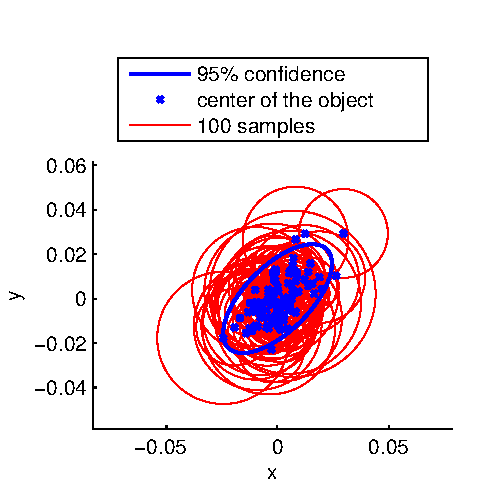
\includegraphics[width=\textwidth]{object_posterior_sample.pdf}
        \caption{A synthetic object posterior $p(x_o|\mathcal{Z} = \mathcal{N}(\mu, \Sigma)$ where $\mu = \left( 0.01,0,0  \right) $ and $\Sigma$ is a covariance matrix with $\sigma_x = \sigma_y = \sigma_r = 0.01$ , $\sigma_{xy} = 0.008$ and $\sigma_{rx} = \sigma_{ry} = 0$ }
        \label{fig:object_posterior_sample}
    \end{subfigure}
    ~ %add desired spacing between images, e. g. ~, \quad, \qquad, \hfill etc. 
      %(or a blank line to force the subfigure onto a new line)
    \begin{subfigure}[b]{0.45\textwidth}
        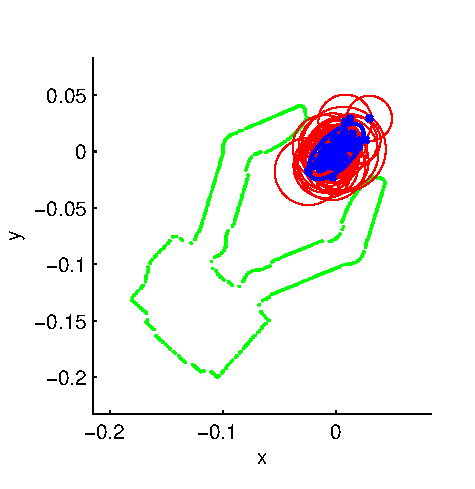
\includegraphics[width=\textwidth]{optimal_pre_touch_conf.pdf}
        \caption{The optimal pre-touch configuration computed for a circular object with the posterior shown to the left. The marginal success probability is $\text{P}(S) = 0.449$.}
        \label{fig:optimal_pre_touch_conf}
    \end{subfigure}
    \caption{An optimal pre-touch configuration computed for a given multivariate Gaussian posterior.}\label{fig:2dexample}
\end{figure}










\section{Modelling perception uncertainty}

%\subsection{Shape-primitive based probability distribution estimation using extended Kalman filter}


\subsection{Surface based probability distribution estimation based on probabilistic fusion}
The aforementioned shape-based approach that aim to represent the object with a limited number of parameter does not scale to real world objects. The reason is that the shapes and surfaces of most real world objects are complex and individual. Grasping these objects requires a robot to have the capability of learning the shape of irregular objects online even the object is presented for the first time. In this section we propose a new method to estimate the probability distribution of the surface of the objects. Rather than predict the shape parameter, this method estimate the course of the object surface achieved by a new probabilistic object representation and a multi-sensor fusion approach. Our surface representation has some significant advantages. First, it models the measurement uncertainty explicitly, as the fusion method explicitly takes Second, the model can be reconstructed with multiple measurements generated by multiple sensors, which have different noise characteristics. Third, one can parallelize the fusion method on GPU, so that the reconstruction
process is performed in real time. Fourth, the efficient query of the surface information allows fast grasp synthesis.

\subsection{Surface representation: p-SDF}
The model of the surface representation is based on signed distance field (SDF). A SDF in a metric space determine the distance between a point and the object surface. The sign of the distance indicates whether the point is outside or inside the object. Besides the distance information we augment the SDF with another additional variable $\sigma$ to represent the uncertainty of the distance. We call this new probabilistic surface representation p-SDF. In this work, a discretized version of p-SDF is used. We discretize a predefined metric space, where p-SDF is defined, into equally sized voxels. We denote the set of all the voxels as $V$. Since the modelling of an object can never be perfect, we have to take the surface uncertainty of modelling into account. To explicitly model the surface uncertainty, we define the distance to each voxel as a normal-distributed random variable. Thus, an object is represented by  
\begin{equation}
\bm{f}: v \mapsto \mathcal{N}(\mu, \sigma^2),  \forall v \in  V ,
\end{equation}
where $\mu$ is the mean and $\sigma$ is the variance of the distribution assigned to voxel $v$.  

\subsection{Surface reconstruction with sensor fusion}
In order to fuse the measurements into the representation using multiple sensors, an iterative method is used to update all the voxel elements. Considering only one voxel $v\in V$, we introduce a  random variables $D_{k}$ associated with voxel $v$. Here, $k$ denotes a time stamp. $\text{Bel}(D_{k-1})$ and $\text{Bel}(D_{k})$ represent the belief signed distance distributions at time stamp $k-1$ and $k$ respectively. We also assume that the major error of one sensor measurement can be approximated as Gaussian white noise, so we can define a measurement model of the sensor by
\begin{equation}
\text{P}(z|c,\Omega) = \mathcal{N}(z^*,  \sigma_\text{sensor}^2), 
\end{equation}
where $c$ denotes a depth camera pose and $\Omega$ denotes the surface of an object. $z^*$ is the true distance between the surface and the depth camera. Furthermore, we denote the true distance between the voxel $v$ to the surface $\Omega$ as $z_\text{sdf}^*$. From Fig.~\ref{fig:sdf} we can derive 
\begin{equation}
z_\text{sdf}^*  = d_{( v,c) } - z^*
\end{equation}
where $d_{( v,c) }$ denotes the distance between the voxel $v$ and the depth camera. Since $z$ follows a Gaussian distribution, $z_\text{sdf}$ also follows a Gaussian distribution, which is given by 
\begin{equation}
\text{P}(z_\text{sdf}|c,\Omega) = \mathcal{N}(z_\text{sdf}^*,  \sigma_\text{sensor}^2).
\end{equation}

\begin{figure}[!htbp]
\centering
\def\svgwidth{0.8\linewidth}
%% Creator: Inkscape inkscape 0.48.3.1, www.inkscape.org
%% PDF/EPS/PS + LaTeX output extension by Johan Engelen, 2010
%% Accompanies image file 'sdf.pdf' (pdf, eps, ps)
%%
%% To include the image in your LaTeX document, write
%%   \input{<filename>.pdf_tex}
%%  instead of
%%   \includegraphics{<filename>.pdf}
%% To scale the image, write
%%   \def\svgwidth{<desired width>}
%%   \input{<filename>.pdf_tex}
%%  instead of
%%   \includegraphics[width=<desired width>]{<filename>.pdf}
%%
%% Images with a different path to the parent latex file can
%% be accessed with the `import' package (which may need to be
%% installed) using
%%   \usepackage{import}
%% in the preamble, and then including the image with
%%   \import{<path to file>}{<filename>.pdf_tex}
%% Alternatively, one can specify
%%   \graphicspath{{<path to file>/}}
%% 
%% For more information, please see info/svg-inkscape on CTAN:
%%   http://tug.ctan.org/tex-archive/info/svg-inkscape
%%
\begingroup%
  \makeatletter%
  \providecommand\color[2][]{%
    \errmessage{(Inkscape) Color is used for the text in Inkscape, but the package 'color.sty' is not loaded}%
    \renewcommand\color[2][]{}%
  }%
  \providecommand\transparent[1]{%
    \errmessage{(Inkscape) Transparency is used (non-zero) for the text in Inkscape, but the package 'transparent.sty' is not loaded}%
    \renewcommand\transparent[1]{}%
  }%
  \providecommand\rotatebox[2]{#2}%
  \ifx\svgwidth\undefined%
    \setlength{\unitlength}{237.96421848bp}%
    \ifx\svgscale\undefined%
      \relax%
    \else%
      \setlength{\unitlength}{\unitlength * \real{\svgscale}}%
    \fi%
  \else%
    \setlength{\unitlength}{\svgwidth}%
  \fi%
  \global\let\svgwidth\undefined%
  \global\let\svgscale\undefined%
  \makeatother%
  \begin{picture}(1,0.57494457)%
    \put(0,0){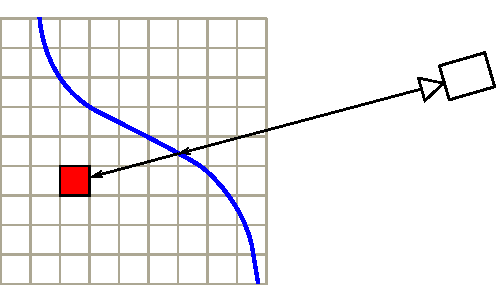
\includegraphics[width=\unitlength]{sdf.pdf}}%
    \put(0.18274527,0.37685155){\color[rgb]{0,0,0}\makebox(0,0)[lb]{\smash{$\Omega$}}}%
    \put(0.59084169,0.36325775){\color[rgb]{0,0,0}\makebox(0,0)[lb]{\smash{$z^*$}}}%
    \put(0.23977624,0.19236224){\color[rgb]{0,0,0}\makebox(0,0)[lb]{\smash{$z_\text{sdf}^*$}}}%
    \put(0.14259879,0.20147031){\color[rgb]{0,0,0}\makebox(0,0)[lb]{\smash{$v$}}}%
    \put(0.89596954,0.33036162){\color[rgb]{0,0,0}\makebox(0,0)[lb]{\smash{$c$}}}%
    \put(0.00452449,0.54940239){\color[rgb]{0,0,0}\makebox(0,0)[lb]{\smash{$V$}}}%
  \end{picture}%
\endgroup%

\caption{Description of the variables that we defined. The grid denotes the volume we consider for modelling an object. $z^*$ is the true measurement from a depth camera. $c$ denotes the pose of the depth camera. $ z_\text{sdf}^*$ is the true signed distance along the direction of the measurement.}
\label{fig:sdf}
\end{figure}	

The belief distribution  $\text{Bel}(D_{k})$ of voxel $v$ can be derived by Bayesian recursive updating by   


\begin{equation}
\begin{split}
\text{Bel}(D_{k}) &= \text{P}(D_{k} | z_\text{sdf}^1,\cdots, z_\text{sdf}^k) \\
                  &= \eta \cdot \text{P}(z_\text{sdf}^k | D_{k} ) \cdot  \text{P}(D_{k-1}|z_\text{sdf}^1\cdots z_\text{sdf}^{k-1} )  \\
                  &= \eta \cdot \text{P}(z_\text{sdf}^k | D_{k} ) \cdot \text{Bel}(D_{k-1})
  \end{split}
\end{equation}   
This equation shows that $\text{Bel}(D_{k})$ can be computed iteratively by the measurement model and the belief prior to the measurement update. In this work, we propose to approximate the belief with a Gaussian distribution for each voxel, so the belief  $\text{Bel}(D_{k})$ can be further computed by 

\begin{equation}
\begin{split}
\text{Bel}(D_{k}) &= \eta \cdot \mathcal{N}(z_\text{sdf},  \sigma_\text{sensor}^2) \cdot  \mathcal{N}( \mu_{k-1} ,   \sigma_{k-1} ^2) \\
&= \eta' \cdot \mathcal{N}( \mu_{k} ,   \sigma_{k} ^2)
  \end{split}
\end{equation}   

with 

\begin{equation}
\label{equ:rule1}
\begin{split}
  {\mu}_{k} &= \frac{{\mu}_{k-1}\cdot\sigma_\text{sensor}^{2}+  z_\text{sdf} \cdot\sigma_{k-1}^{2}}{\sigma_{k-1}^{2}+\sigma_\text{sensor}^2}
\end{split}
\end{equation}
%
\begin{equation}
\label{equ:rule2}
\begin{split}
  \sigma_{k}^{2} &=\frac{\sigma_{k-1}^{2}\cdot\sigma_\text{sensor}^2}{\sigma_{k-1}^{2}+\sigma_\text{sensor}^2}.
\end{split}
\end{equation}
We use Equ.~\ref{equ:rule1} and Equ.~\ref{equ:rule2} to update the whole volume $V$. To update the volume with another depth camera, one only needs to exchange $\sigma_\text{sensor}^2$ to the variance which represents the measurement characteristics of the camera. 



\section{Searching for feasible grasp configuration}

In general, numerous pre-touch configurations are feasible for a successful grasp, since most objects can be stably grasped in different ways. The marginal probability $P(s|g_n,\bm{f})$ is a high-dimensional non-convex function with respect to $g_n$. $g_n$ is parameterized by the pose of the gripper relatively to the object and the positions of joints. Finding the optimum of $g_n$ is not trivial. We propose to solve this problem in two steps. First, we use a generalizable method to parametrize the grasp posture which reduces the dimension of gripper configurations. The parametrization is then used in a two-stage search method, which involves sampling a number of configurations to evaluate the success probability and refining the configuration of the best sample.    

\subsection{Reducing configuration space of grippers using synergy }

We follow the concept of `eigen-grasp'\cite{Ciocarlie2009} to parameterize the gripper. This concept is based on the grasp synergy which allows the joint positions to be controlled only by a subspace of the total available degrees of freedom. In our work, we use grippers with more than two degrees of freedom (DOF). Given a gripper with $d$ DOF, we organize joints on the same finger into a group so that only one parameter is required to control the whole finger. We define the set of joint groups as $\mathbb{J}$. Later we use this reduced parameter space to search for grasps. After defining the groups, we define a set of grasp types $\mathbb{T}$ that are feasible for the gripper. Typically, these grasp types indicate which grasp type is reasonable for a specific object or a specific task, e.g. a pinch grasp is more suitable for grasping a chopstick than a power grasp. A grasp type is parametrized by an opening posture $P_b \in\mathbb{R}^d$  and a closing posture $P_e \in\mathbb{R}^d$. To generate a gripper configuration of a particular type, we must first compute an eigen grasp matrix  $M$ for this type. The algorithm for computing $M$ is given by Algorithm \ref{alg1}. 

\begin{algorithm}
\begin{algorithmic}[1]
\STATE Input:  $\mathbb{J}$, $P_b$, $P_e$, $d$   
\STATE $n_g  =  |\mathbb{J}| $
\STATE $k = 0$ % joint index
\STATE $r = 0$ % row begin 
\STATE resize $M$ to $d$ rows and $n_g$ columns  
\FOR {$i$ from 1 to $n_g$}
\FOR {$j$ from 1 to $\mathbb{J}$[i] }
\STATE row = $r + j$ 
\STATE col = $i$   
\STATE $M$(row, col) = $P_e[k] - P_b[k]$
\STATE $k = k + 1$
\ENDFOR
\STATE $r = r + n_g$
\ENDFOR
\RETURN $M$
%\captionsetup{justification=raggedright}
\caption {Compute $M_t$ of grasp type $t$}
\label{alg1}
\end{algorithmic}
\end{algorithm}

The entire joint configuration of a grasp $\bm{j}$ is computed by 
\begin{equation}
\bm{j} = M \cdot \alpha + P_b
\label{equ:eigen_grasp}
\end{equation}
where $M$ is a $d \times n_g$ matrix, $\alpha$ is a $n_g \times 1$ vector and $n_g$ is the number of groups we defined for the gripper. Also note that $\forall \alpha_i \in \alpha, \alpha_i$ is defined in $[0,1]$. Thus the joint configuration $j$ equals $P_b$ when $\forall \alpha_i \in \alpha$, $\alpha_i = 0$ and equals $P_e$ when $\forall \alpha_i \in \alpha$, $\alpha_i = 1$. 

\begin{figure}[!htbp]
\centering
\def\svgwidth{1\linewidth}
%% Creator: Inkscape inkscape 0.48.3.1, www.inkscape.org
%% PDF/EPS/PS + LaTeX output extension by Johan Engelen, 2010
%% Accompanies image file 'grasp_types_new.pdf' (pdf, eps, ps)
%%
%% To include the image in your LaTeX document, write
%%   \input{<filename>.pdf_tex}
%%  instead of
%%   \includegraphics{<filename>.pdf}
%% To scale the image, write
%%   \def\svgwidth{<desired width>}
%%   \input{<filename>.pdf_tex}
%%  instead of
%%   \includegraphics[width=<desired width>]{<filename>.pdf}
%%
%% Images with a different path to the parent latex file can
%% be accessed with the `import' package (which may need to be
%% installed) using
%%   \usepackage{import}
%% in the preamble, and then including the image with
%%   \import{<path to file>}{<filename>.pdf_tex}
%% Alternatively, one can specify
%%   \graphicspath{{<path to file>/}}
%% 
%% For more information, please see info/svg-inkscape on CTAN:
%%   http://tug.ctan.org/tex-archive/info/svg-inkscape
%%
\begingroup%
  \makeatletter%
  \providecommand\color[2][]{%
    \errmessage{(Inkscape) Color is used for the text in Inkscape, but the package 'color.sty' is not loaded}%
    \renewcommand\color[2][]{}%
  }%
  \providecommand\transparent[1]{%
    \errmessage{(Inkscape) Transparency is used (non-zero) for the text in Inkscape, but the package 'transparent.sty' is not loaded}%
    \renewcommand\transparent[1]{}%
  }%
  \providecommand\rotatebox[2]{#2}%
  \ifx\svgwidth\undefined%
    \setlength{\unitlength}{221.55bp}%
    \ifx\svgscale\undefined%
      \relax%
    \else%
      \setlength{\unitlength}{\unitlength * \real{\svgscale}}%
    \fi%
  \else%
    \setlength{\unitlength}{\svgwidth}%
  \fi%
  \global\let\svgwidth\undefined%
  \global\let\svgscale\undefined%
  \makeatother%
  \begin{picture}(1,0.57628075)%
    \put(0,0){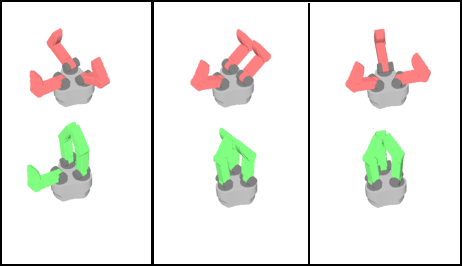
\includegraphics[width=\unitlength]{grasp_types_new.pdf}}%
    \put(0.09508525,0.04601723){\color[rgb]{0,0,0}\makebox(0,0)[lb]{\smash{pinch}}}%
    \put(0.45764631,0.04601723){\color[rgb]{0,0,0}\makebox(0,0)[lb]{\smash{cylindrical}}}%
    \put(0.8037149,0.04601723){\color[rgb]{0,0,0}\makebox(0,0)[lb]{\smash{spherical}}}%
  \end{picture}%
\endgroup%

%\captionsetup{justification=centering}
\caption{Three grasp types are defined for SCHUNK-SDH gripper. The fingers of the gripper for an opening grasp posture $P_b$ are marked in red, the ones for a closing grasp posture $P_e$ are marked in green.}
\label{fig:grasp_types}
\end{figure}	

Fig.~\ref{fig:grasp_types} depicts an example how we parametrize a SCHUNK-SDH gripper. SCHUNK-SDH has a total of three fingers. Each of them has two joints with independent actuators. Two of three fingers have an additional joint at the finger root. These two joints are driven by the same actuator to change the directions of force closure. We define in total three grasp types and their corresponding parameters $P_b$ and $P_e$. We organize two joints on the same finger into one group and additionally the two coupled joints into another group. The total amount of the joint groups add up to four for this gripper. In this work, we focus ourself on the pinch grasp only, since it mimics the most widely used parallel gripper and is capable of grasping a large amount types of objects.  

\todo{another example with Robotiq gripper}


\subsection{Calculation of surface normals}
Surface normals on the desired contact points are used to evaluate the conditional grasp success probability. For irregular objects which can be represented by p-SDF, the surface element can be accessed by an operation called ray-casting. Ray casting evaluates the function along a given direction until a zero-crossing is found. To employ this method for grasp generation, we attach a set of frames organized by a grid to each finger tip. These frames are then used as a set of simulated proximity sensors to determine the distance between finger tips and the object surface. The region covered by these frames can be considered as a desired contact patch region. Fig. \ref{fig:simulated_sensor} depicts a realization of simulated proximity sensors on a SCHUNK-SDF Gripper.

\begin{figure}
\centering
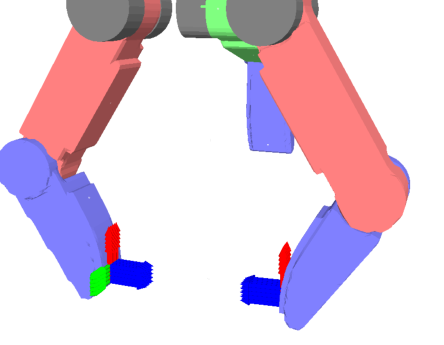
\includegraphics[width=0.4\linewidth]{camera_frame2.pdf}
\captionsetup{justification=raggedright}
\caption{For each finger tip, 25 Frames are attached to the region, where contacts and forces are applied during grasping.}
\label{fig:simulated_sensor}       % Give a unique label
\end{figure}   

Given an object modeled by p-SDF and a pre-touch configuration of a gripper, the desired contact normals are evaluated by first conducting ray casting for each frame. We obtain 25 desired contact points which forms a contact region.  We use these points as inputs for a RANSAC plane segmentation \cite{Zuliani2008}. The contact region is regarded as feasible, if at least 20 points are considered as inlier of a plane. This rules out unstable contact region where the course of an object surface is not smooth. The normal of the contact can be calculated from the plane segmentation result. In this way, we avoid using a point-contact model to evaluate contacts but use a contact patch for estimating the contacts and contact normals. This simulates physical contacts in a real grasping scenario. Stable contacts are usually established between a region of two surfaces not a point.  Fig.~\ref{fig:bunny_raycast} depicts the result of the contact points (magenta) and surface normals (yellow arrows) determined by ray casting.

\begin{figure}
\centering
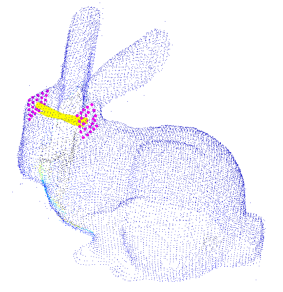
\includegraphics[width=0.4\linewidth]{bunny_raycast_new.pdf}
\captionsetup{justification=raggedright}
\caption{Desired contact positions of a pre-touch configuration determined by ray casting. Magenta: contact points, yellow arrows: surface normals. For  the purpose of visualization, this model is generated in Gazebo simulation.}
\label{fig:bunny_raycast}       % Give a unique label
\end{figure} 


\subsection{A two-stage method for grasp synthesis}
The objective function $P(S | g_n, \bm{f})$ to be maximized is in general non-linear and non-convex. Directly searching in the parameter space tends to find local optimal solutions. The parameter space of $g_n = \lbrace \bm{p}, \bm{\alpha} \rbrace $ contains a pose parameter $\bm{p}$ in $\mathbb{R}^6$ and a posture parameter $\bm{\alpha}$ in $\mathbb{R}^{N_g}$. The pose parameter can be used to place the gripper at an almost satisfactory region, in which simulated proximity sensors have valid measurements,  while the posture parameter is used for the fine adjustment of the finger tips. In algorithm 2, we propose a two-stage method to generate the pre-touch configuration. In the first stage, we sample a set of new poses based on an input parameter $\Delta d$ from a uniform distribution. $\Delta d$ can be chosen as the largest length of the bounding box of the object, which we obtained from a segmented point cloud. Then we apply the offsets sampled from the distribution to the initial configuration $g_{\text{init}}$ to generate a set of sample configurations. All the samples are then evaluated in Line 9 and 10. The function IK$(g_{\text{sample}})$ checks if the sample configuration is reachable of the robot and collision-free from the environment. The sample with the largest marginal success probability is then passed to stage 2 of the algorithm. In stage 2, we refine the pre-touch configuration from the result of stage 1.  We sample the poses within the XZ plane of the gripper by parameter $\Delta d_r$. We choose parameter $\Delta d_r$ to be sufficiently small (e.g 1 cm) but still give the algorithm the opportunity to find a better pre-touch configuration. The intuition behind that is a better pre-touch configuration can be found within a neighbored region of pose of the $g^*$ from stage 1. From Line 25 to Line 29, we evaluate the distance from the finger tips to the surface and use this information to iteratively search for the posture parameter $\bm{\alpha}$ until the distance is within the threshold of a desired pre-touch configuration distance $d_{\text{pre}}$.

\begin{figure}[!htbp]
\centering
\def\svgwidth{0.4\linewidth}
%% Creator: Inkscape inkscape 0.48.4, www.inkscape.org
%% PDF/EPS/PS + LaTeX output extension by Johan Engelen, 2010
%% Accompanies image file 'algorith_help.pdf' (pdf, eps, ps)
%%
%% To include the image in your LaTeX document, write
%%   \input{<filename>.pdf_tex}
%%  instead of
%%   \includegraphics{<filename>.pdf}
%% To scale the image, write
%%   \def\svgwidth{<desired width>}
%%   \input{<filename>.pdf_tex}
%%  instead of
%%   \includegraphics[width=<desired width>]{<filename>.pdf}
%%
%% Images with a different path to the parent latex file can
%% be accessed with the `import' package (which may need to be
%% installed) using
%%   \usepackage{import}
%% in the preamble, and then including the image with
%%   \import{<path to file>}{<filename>.pdf_tex}
%% Alternatively, one can specify
%%   \graphicspath{{<path to file>/}}
%% 
%% For more information, please see info/svg-inkscape on CTAN:
%%   http://tug.ctan.org/tex-archive/info/svg-inkscape
%%
\begingroup%
  \makeatletter%
  \providecommand\color[2][]{%
    \errmessage{(Inkscape) Color is used for the text in Inkscape, but the package 'color.sty' is not loaded}%
    \renewcommand\color[2][]{}%
  }%
  \providecommand\transparent[1]{%
    \errmessage{(Inkscape) Transparency is used (non-zero) for the text in Inkscape, but the package 'transparent.sty' is not loaded}%
    \renewcommand\transparent[1]{}%
  }%
  \providecommand\rotatebox[2]{#2}%
  \ifx\svgwidth\undefined%
    \setlength{\unitlength}{101.7223632bp}%
    \ifx\svgscale\undefined%
      \relax%
    \else%
      \setlength{\unitlength}{\unitlength * \real{\svgscale}}%
    \fi%
  \else%
    \setlength{\unitlength}{\svgwidth}%
  \fi%
  \global\let\svgwidth\undefined%
  \global\let\svgscale\undefined%
  \makeatother%
  \begin{picture}(1,1.11202323)%
    \put(0,0){\includegraphics[width=\unitlength]{algorith_help.pdf}}%
    \put(0.61706548,0.89542968){\color[rgb]{0,0,0}\makebox(0,0)[lb]{\smash{xz plane}}}%
    \put(0.43200533,0.02430309){\color[rgb]{0,0,0}\makebox(0,0)[lb]{\smash{x}}}%
    \put(0.66835092,0.01635887){\color[rgb]{0,0,0}\makebox(0,0)[lb]{\smash{y}}}%
    \put(0.5572892,0.21926022){\color[rgb]{0,0,0}\makebox(0,0)[lb]{\smash{z}}}%
  \end{picture}%
\endgroup%

%\captionsetup{justification=centering}
\caption{Parametrization for refining a pre-touch configuration.}
\label{fig:algorith_help}
\end{figure}	



\begin{algorithm}
\begin{algorithmic}[1]
\STATE Input: $\bm{f} $, $g_{\text{init}}$,  $N_{\text{sample}}$ , $N_{\text{refine}}$, $\Delta d$ , $\Delta d_r$, $d_{\text{pre}}$
\STATE $P^{*} = 0$
\STATE $\Delta \bm{\alpha} = [0.01, 0.01]$
\STATE // stage 1.
\FOR { $i$ from 1 to $N_{\text{sample}}$ } 
\STATE   Sample offsets $\Delta x^{*}$,$\Delta y^{*}$,$\Delta z^{*}$ from  Unif(-$\frac{\Delta d}{4} ,+ \frac{\Delta d}{4}$)
\STATE   Sample $\Delta \beta$ from Unif(-$\pi ,+ \pi$)
\STATE   $g_{\text{sample}} \leftarrow $ Apply position offsets and  rotation offset $\Delta \beta$ to $g_{\text{init}}$ 
\STATE  $P_i = P(S | g_{\text{sample}}, \bm{f})$
\IF {  $P_i > P^{*} $ and IK  ($g_{\text{sample}}$ ) is True}
\STATE $P^{*} = P_i$
\STATE $g^{*} = g_{\text{sample}} $
\ENDIF  
\ENDFOR 
\STATE // stage 2
\FOR { $j$ from 1 to $N_{\text{refine}}$ } 
\STATE Sample an offset from Unif( -$\Delta d_r$ ,$\Delta d_r$ )
\STATE $g_{\text{refine}} \leftarrow $ Apply the offset to pose of $g^{*}$ in xz plane (see. Fig.~\ref{fig:algorith_help})  
\STATE  $P_{\text{refine}} = P(S | g_{\text{refine}}, \bm{f})$
\IF {  $P_{\text{refine}} > P^{*} $ }
\STATE $P^{*} = P_{\text{refine}}$
\STATE $g^{*} = g_{\text{refine}} $
\ENDIF
\ENDFOR
\STATE $(d_1,d_2) = \text{raycast}(g^*, \bm{f})$
\WHILE { $ |d_1 - d_{\text{pre}}| > 1 mm$ or $ |d_2 - d_{\text{pre}}| >1 mm$ }
\STATE $y_{(g^{*})} = y_{(g^{*})} + \frac{d_1-d_2}{2} $ 
\STATE $ \bm{\alpha}_{(g^*)} = \bm{\alpha}_{(g^*)} + \Delta \bm{\alpha}$ 
\STATE $(d_1,d_2) = \text{raycast}(g^*, \bm{f})$
\ENDWHILE
\RETURN $g*$
\caption {A two-stage pre-touch generation algorithm for pinch grasp}
\end{algorithmic}
\end{algorithm}

\section{Experimental evaluation: Grasping unknown objects}
We choose a challenging task, grasping of unknown objects, to validate the proposed approach. Unknown objects are the objects which are presented to a robot for the first time. All of the objects we chose for this experiment have their individual shapes, which additionally increase the difficulty. In the following, we first introduce the experimental setup, followed by the evaluation of the algorithm and the performance evaluation of the overall grasping accuracy. 

\subsection{Experimental setup}
The test objects that we used in the experiment are shown in Fig.~\ref{fig:test_objects}. Every time we place one object on the table. The robot is required to lift the object 10 cm above the table. If the robot grasps the object successfully, it rotates its wrist of a random angle and places the object back to start a new grasping attempt. For each object the robot repeats the experiment autonomously for 20 attempts. Human intervention is only involved if the robot fails to pick up an object. In the case that the robot does not recognize the failure and continues to place back the object,  we manually remove the object to prevent the robot from breaking its gripper.  

\begin{figure}[!htbp] 
\centering
\includegraphics[width=0.7\linewidth]
{figure/test_object.png}%\captionsetup{justification=centering}
\caption{Test objects we used in this experiment. From left to right: a 3-D printed `bunny', `big duck', `tape rectangular', `tape triangle', `stapler', `toy car', `duckie', `screwdrawer', `PS3 joystick', `correction fluid'. }
\label{fig:test_objects}
\end{figure}	
   
\subsubsection{Hardware}
We conduct the experiments with a fully integrated mobile manipulation robot (Care-o-bot) \todo {[cite]}. The robot is equipped with a 7 DOF KUKA lightweight robot with a 7 DOF SCHUNK-SDH gripper mounted on the wrist. The robot is driven by an omni-directional mobile platform. The primary sensors of the robot include a head-mounted Microsoft Kinect sensor and a
hand-mounted stereo camera (Ensenso N10). More details of other hardware components can be found in attachment. \todo {ref}

\subsubsection{Object modelling}
Prior to each grasp attempt, the robot moves its gripper to several pre-defined poses so that the object is perceived from both head camera (Kinect) and in-hand camera (Ensenso). During the movement, our fusion algorithm integrates the measurements simultaneously from both cameras. Fig.~\ref{fig:time_evolution} illustrates the process of modelling the `toy car' by moving the gripper relatively slowly. For the first 9 s, the top side of the object is visible to the in-hand camera, so the uncertainty of the top region is reduced gradually. The black area of the object indicates that the region of wheels is still under large uncertainty. After 9 s the robot moves the in-hand camera to some other view points to acquire more information about the region of wheels. Fig.~\ref{fig:numberofframes} shows the number of frames used to fuse the object during the entire modelling process.  

\todo {add more examples like bunny duckie etc.}

\begin{figure}[!htbp]
\centering
%\def\svgwidth{1\linewidth}
\includegraphics[width=1\linewidth]{figure/time_evolution.png}%\captionsetup{justification=centering}
%%% Creator: Inkscape inkscape 0.48.4, www.inkscape.org
%% PDF/EPS/PS + LaTeX output extension by Johan Engelen, 2010
%% Accompanies image file 'time_evolution.pdf' (pdf, eps, ps)
%%
%% To include the image in your LaTeX document, write
%%   \input{<filename>.pdf_tex}
%%  instead of
%%   \includegraphics{<filename>.pdf}
%% To scale the image, write
%%   \def\svgwidth{<desired width>}
%%   \input{<filename>.pdf_tex}
%%  instead of
%%   \includegraphics[width=<desired width>]{<filename>.pdf}
%%
%% Images with a different path to the parent latex file can
%% be accessed with the `import' package (which may need to be
%% installed) using
%%   \usepackage{import}
%% in the preamble, and then including the image with
%%   \import{<path to file>}{<filename>.pdf_tex}
%% Alternatively, one can specify
%%   \graphicspath{{<path to file>/}}
%% 
%% For more information, please see info/svg-inkscape on CTAN:
%%   http://tug.ctan.org/tex-archive/info/svg-inkscape
%%
\begingroup%
  \makeatletter%
  \providecommand\color[2][]{%
    \errmessage{(Inkscape) Color is used for the text in Inkscape, but the package 'color.sty' is not loaded}%
    \renewcommand\color[2][]{}%
  }%
  \providecommand\transparent[1]{%
    \errmessage{(Inkscape) Transparency is used (non-zero) for the text in Inkscape, but the package 'transparent.sty' is not loaded}%
    \renewcommand\transparent[1]{}%
  }%
  \providecommand\rotatebox[2]{#2}%
  \ifx\svgwidth\undefined%
    \setlength{\unitlength}{586.66371111bp}%
    \ifx\svgscale\undefined%
      \relax%
    \else%
      \setlength{\unitlength}{\unitlength * \real{\svgscale}}%
    \fi%
  \else%
    \setlength{\unitlength}{\svgwidth}%
  \fi%
  \global\let\svgwidth\undefined%
  \global\let\svgscale\undefined%
  \makeatother%
  \begin{picture}(1,0.29084708)%
    \put(0,0){\includegraphics[width=\unitlength]{time_evolution.pdf}}%
    \put(0.83802275,0.00384053){\color[rgb]{0,0,0}\makebox(0,0)[lb]{\smash{t[s]}}}%
    \put(0.94944208,0.24723034){\color[rgb]{0,0,0}\makebox(0,0)[b]{\smash{$0,0 mm$}}}%
    \put(0.95416081,0.03165352){\color[rgb]{0,0,0}\makebox(0,0)[b]{\smash{$10,0 mm$}}}%
    \put(0.94522098,0.13221012){\color[rgb]{0,0,0}\makebox(0,0)[b]{\smash{$5 mm$}}}%
    \put(0.08301408,0.00116712){\color[rgb]{0,0,0}\makebox(0,0)[lb]{\smash{1}}}%
    \put(0.27178126,0.00019309){\color[rgb]{0,0,0}\makebox(0,0)[lb]{\smash{6}}}%
    \put(0.44087302,0.00019309){\color[rgb]{0,0,0}\makebox(0,0)[lb]{\smash{9}}}%
    \put(0.61132843,0.00175154){\color[rgb]{0,0,0}\makebox(0,0)[lb]{\smash{25}}}%
    \put(0.77886175,0.00097229){\color[rgb]{0,0,0}\makebox(0,0)[lb]{\smash{30}}}%
  \end{picture}%
\endgroup%

\caption{The process of modelling a `toy car'. Top: The robot moves its in-hand camera to several pre-defined poses to see the object from different viewing angles. Middle: Raycasted views of the model are shown alongside each robot pose. Bottom: A colorized model of the object visualizes the uncertainty of the object during the modelling process. In the first three figures, the black points on the wheels indicate a large uncertainty on those regions, because the object was only observed from its top.}
\label{fig:time_evolution}
\end{figure}

\begin{figure}[!htbp]
\centering
\def\svgwidth{0.7\linewidth}
%% Creator: Inkscape inkscape 0.48.4, www.inkscape.org
%% PDF/EPS/PS + LaTeX output extension by Johan Engelen, 2010
%% Accompanies image file 'numberofframessvg.pdf' (pdf, eps, ps)
%%
%% To include the image in your LaTeX document, write
%%   \input{<filename>.pdf_tex}
%%  instead of
%%   \includegraphics{<filename>.pdf}
%% To scale the image, write
%%   \def\svgwidth{<desired width>}
%%   \input{<filename>.pdf_tex}
%%  instead of
%%   \includegraphics[width=<desired width>]{<filename>.pdf}
%%
%% Images with a different path to the parent latex file can
%% be accessed with the `import' package (which may need to be
%% installed) using
%%   \usepackage{import}
%% in the preamble, and then including the image with
%%   \import{<path to file>}{<filename>.pdf_tex}
%% Alternatively, one can specify
%%   \graphicspath{{<path to file>/}}
%% 
%% For more information, please see info/svg-inkscape on CTAN:
%%   http://tug.ctan.org/tex-archive/info/svg-inkscape
%%
\begingroup%
  \makeatletter%
  \providecommand\color[2][]{%
    \errmessage{(Inkscape) Color is used for the text in Inkscape, but the package 'color.sty' is not loaded}%
    \renewcommand\color[2][]{}%
  }%
  \providecommand\transparent[1]{%
    \errmessage{(Inkscape) Transparency is used (non-zero) for the text in Inkscape, but the package 'transparent.sty' is not loaded}%
    \renewcommand\transparent[1]{}%
  }%
  \providecommand\rotatebox[2]{#2}%
  \ifx\svgwidth\undefined%
    \setlength{\unitlength}{213.55739336bp}%
    \ifx\svgscale\undefined%
      \relax%
    \else%
      \setlength{\unitlength}{\unitlength * \real{\svgscale}}%
    \fi%
  \else%
    \setlength{\unitlength}{\svgwidth}%
  \fi%
  \global\let\svgwidth\undefined%
  \global\let\svgscale\undefined%
  \makeatother%
  \begin{picture}(1,0.41857128)%
    \put(0,0){\includegraphics[width=\unitlength]{numberofframessvg.pdf}}%
    \put(0.49756185,0.01128552){\makebox(0,0)[lb]{\smash{\small{t[s]}}}}%
    \put(0.09282368,0.08132461){\makebox(0,0)[lb]{\smash{0}}}%
    \put(0.06443245,0.20731075){\makebox(0,0)[lb]{\smash{50}}}%
    \put(0.03604122,0.33329678){\makebox(0,0)[lb]{\smash{100}}}%
    \put(0.35378421,0.29015447){\makebox(0,0)[lb]{\smash{kinect}}}%
    \put(0.35378421,0.23448302){\makebox(0,0)[lb]{\smash{ensenso}}}%
    \put(0.27065576,0.05747682){\makebox(0,0)[lb]{\smash{1}}}%
    \put(0.41567291,0.05916184){\makebox(0,0)[lb]{\smash{6}}}%
    \put(0.55919591,0.06036764){\makebox(0,0)[lb]{\smash{9}}}%
    \put(0.69462102,0.05909079){\makebox(0,0)[lb]{\smash{25}}}%
    \put(0.83415963,0.05814475){\makebox(0,0)[lb]{\smash{30}}}%
    \put(0.02193696,0.08258763){\rotatebox{90}{\makebox(0,0)[lb]{\smash{\small{Number of frames}}}}}%
  \end{picture}%
\endgroup%

\caption{Number of frames used to model the 'toy car' (object see in Fig.~ \ref{fig:test_objects}). The time stamp of each bar corresponds to that of modelling result in Fig.~\ref{fig:time_evolution}.}
\label{fig:numberofframes}
\end{figure}

\subsection{Performance evaluation on grasp synthesis algorithm}
To generate a viable grasp we first fit a bounding box to a point cloud that is segmented from the table. Based on the estimate of bounding box, we compute for each object an initial pinch grasp, which is aligned to the bounding box. The initial grasp is used
to initialize the grasp synthesis algorithm. We evaluate the performance of grasp generation in terms of the number of samples. Fig.~\ref{fig:algo_runtime} depicts the time consumption to compute a grasp with different number of samples. The computation time increases linear with the number of grasp samples. We get the variance of time consumption by running the algorithm 10 times for a fixed number of samples. By evaluating the algorithm on three different objects, we also show that the computation time is not correlated to the object type. Fig.~\ref{fig:algo_prob} illustrates the maximum success probability with respect to the number of samples. The maximum success probability can be found after evaluating approximate 200 samples, which means our algorithm can find a viable grasp within 2 seconds. Compared to the result of a similar work \todo{\cite{mahler2015}[]}, who also uses signed distance function to model objects, our algorithm is at least 30 times faster.

\begin{figure}[!htpb]
\centering
\includegraphics[width=0.7\linewidth]{figure/algo_runtime2-crop.pdf}
\caption{The mean computation time of the grasp generation algorithm scales linearly with the number of samples. The variance is computed by evaluating 10 times for a given number of samples.}
\label{fig:algo_runtime}
\end{figure}


\begin{figure}[!htpb]
\centering
\includegraphics[width=0.7\linewidth]{figure/algo_prob2-crop.pdf}
\caption{The algorithm converges approximately by evaluating 200 samples.}
\label{fig:algo_prob}
\end{figure}


\subsection{Performance on grasping accuracy}
In our experiments, we define three types of outcomes to judge a grasping attempt. They are success with precision (S.w.P),  success (S.) and failure (F). S.w.P means the object is successfully picked up and placed back while the gripper does not displace the object more than 1 cm or more than 30 degree during force closure. An outcome is marked as S., when the object is successfully picked up in spite of being displaced or rotates within the gripper. An attempt is marked as failure if the object is not successfully picked up or slips out of the gripper. 

Table \ref{tab:result} summarizes the result for a total number of 200 grasping attempts. Our algorithm has achieved 93.5\% success rate of lifting the objects and 79.5 \%  success rate of grasping with precision. The robot manages to grasp 'duckie' and 'correction fluid' without failure. 7 objects are successfully grasped with only a single failure. Fig.~\ref{fig:grasp_example} illustrates some successful grasps generated from our algorithm. 

Among all the objects we used in the experiments, `PS3 Joystick' is the most difficult object for the robot to pick up. Depending on the viewing angle, the hand-mounted Ensenso stereo camera sometimes does not provide reliable depth images so that the object model is only partially integrated or the integration contains large uncertainty. Noted that there is only a few viable pinch grasps which can be used to lift the `PS3 Joystick'. These viable grasps are all located at the middle. When the contact regions for these viable grasps are not well modelled or have large uncertainty, our algorithm is not capable of finding them. These phenomena are also observed for the `screw drawer' and the `stapler'. For these two objects, the region where the surface is black results in a large uncertainty in the model. Since these objects contain more feasible grasps, our robot still manages to pick up them successfully. However, the robot has a lower success rate on these objects if S.w.P criterion is used to assess the grasp outcome. Fig.~\ref{fig:slip_staple} depicts one common grasp generated from our algorithm for the `stapler'. Our algorithm tends to find grasps at the end side  of the `stapler', because that region are well modelled and certain to the robot. Since this grasp cannot counteract the wrench generated by the gravity, as soon as the object is lifted up, an in-gripper  object rotation may happen.   

\begin{figure}[!htpb]
\centering
\includegraphics[width=0.7\linewidth]{figure/non_optimal_grasp.pdf}
\caption{(a) A grasp generated by our algorithm for the 'stapler'. Our algorithm tends to generate grasp in the region where the uncertainty is small, which leads to an non-optimal grasp for this case. This grasp may lead to an in-gripper rotation, because it cannot counteract the wrench of gravity. (b) The black points indicate that the side surface of the object has a large uncertainty, however these regions are the only good contact region for a stable grasp. Since our algorithm avoids to generate grasps on uncertainty surfaces, an non-stable grasp is found at one control axis of the `PS3 Joystick'.}
\label{fig:slip_staple} 
\end{figure}

\begin{figure*}[!htpb]
\centering
\includegraphics[width=0.8\linewidth]{figure/successful_grasps_illustration.pdf}
\caption{Grasps generated by the algorithm with successful execution.}
\label{fig:grasp_example} 
\end{figure*}

\begin{figure*}[!htpb]
\centering
\includegraphics[width=0.8\linewidth]{figure/success_grasp_real.pdf}
\caption{Successful grasps executed by the robot. }
\label{fig:success_grasps}
\end{figure*}



\begin{table}[!htpb]
\centering
\begin{tabular}{lrrr}
Object           & \multicolumn{1}{c}{S.} & \multicolumn{1}{c}{F.} & \multicolumn{1}{c}{S.w.P} \\
Bunny            & 19/20                  & 1/20                   & 15/20                     \\
Big duck         & 19/20                  & 1/20                   & 16/20                     \\
Tape rectangular & 19/20                  & 1/20                   & 19/20                     \\
Tape triangle    & 19/20                  & 1/20                   & 19/20                     \\
Stapler          & 19/20                  & 1/20                   & 14/20                     \\
Toy car          & 19/20                  & 1/20                   & 18/20                     \\
Duckie           & 20/20                  & 0/20                   & 20/20                     \\
Screwdrawer      & 19/20                  & 1/20                   & 11/20                     \\
PS3 Joystick     & 14/20                  & 6/20                   & 7/20                      \\
Correction fluid & 20/20                  & 0/20                   & 20/20                     \\
Summary          & \textbf{93.5\%}        & 6.5\%            & \textbf{79.5\%}                  
\end{tabular}
\caption{(S. = success, F. = failure, S.w.P = Success with precision). Experimental result for a total of 200 grasping attempts. An outcome is classified as S.w.P when gripper successfully picked the object without displacing the object more than 1 cm or 30 degree. This criterion is strict comparing to a standard way to access grasping success.} 
\label{tab:result}
\end{table}


\subsection{Discussion} 
Precise grasping is one of the advantages of the proposed
approach. By explicitly modelling the surface geometry and
its uncertainty, we can compute grasps with more precision
so that during force closure the object is less probable to be displaced. Due to the unknown dynamics of the object, displacement of the object may result in grasp failure more likely, when unexpected situation such as slipping happens.

Most approaches address the problem of grasping unknown object by finding grasp relevant feature from a single measurement. Single measurement however may contain large uncertainty. Partial and occlusion of the measurement usually results in a hard situation for grasp detection. Well defined grasp features such as surface normals can not be used, because the region where contacts take place are usually not observable from a single measurement. Our approach handles this problem by integrating multiple measurements so that we can use well defined features, namely, the surface normals and the modelling uncertainty to assess the viability of grasps. 

Recently, some approaches exploit large neuron network to learn grasp features large scale grasping experiments \cite{pinto2015supersizing}. Gathering grasping experience with this method is very expensive, it requires to run robot in very long time. Our approach requires neither training or learning, and still gets a competitive result. This indicates that the choice of a good representation improves the system performance dramatically. 

There are also some limitations in the current approach. Our approach can not handle transparent objects such as `glasses', `coins', `small screws'. In these cases, exploiting other sensing modality such as a color camera may help. Another drawback of our approach is that the robot requires to observe the objects with different pre-defined view angles prior to grasping, this may increase the time of task execution. Regarding this problem, one may exploit active perception approaches to minimize the travel distance while still acquiring sufficient information for a stable grasp. 


\cleardoublepage
\thispagestyle{empty}
\chapter{An Adaptive Grasping Control Architecture for Whole Body Mobile Manipulation} \label{chapter_control}
Humans use eye and touch to monitor the entire process of grasping. They can change the grasping strategy on the fly when needed. This is why humans are capable of grasping objects very robustly. 
In this chapter, we address the problem of grasp execution and demonstrate how the grasping can be executed robustly under limited sensing capability.  

\section{Introduction}
Grasp execution is one of the most important steps for grasping success. Many earlier works use vision, tactile sensing, proximity sensing to improve the robustness of grasp execution (\cite{Felip2009},\cite{Hsiao2010},\cite{Hudson2012},\cite{jiang2012seashell}). Grasp execution on a real robot can be used to test whether the planned grasp configuration is feasible or not. Due to the error of object localization, sensor calibration and uncertain robot motion, the actual grasping configuration may differ from the planned one. Therefore, we need to handle these errors and keep the actual grasp configuration as close as possible to the intended one. 

Many approaches (\cite{Kamon1996},\cite{Rao2010},\cite{Roa2009}) which address the grasping problem usually assume perfect executions. They usually follow a sense-plan-action paradigm to execute a grasp. In the sensing phase, a robot recognizes, localizes and segments a desired object from the environment. In the planning phase, grasping points and grasping trajectory are calculated. In the action phase, the robot executes the  planned grasping trajectory to perform the grasp, usually in open-loop. One problem related to this paradigm is, sensing of object's state is missing in the action phase. If the action phase takes more than several seconds  without updating the object's state, the robot is unable to react to actuation error or external perturbation. Humans also use this paradigm to perform grasping but the sense-plan-action cycling time is much shorter. They maintain eye contact to the object until the object is fetched. In addition, they can adapt their grasp motion when object is displaced. In order to achieve maximal efficiency, humans seamlessly combine their locomotion, body, and arm movement for the entire grasping process.

In this chapter, we propose a flexible and adaptive grasping control architecture to imitate  human grasping. The flexibility is reflected in the freedom of choice and combination of  required actuators in different grasping phases. We define three grasping phases for the entire grasp execution process as shown in Fig.~\ref{fig:grasping_process}. During the initial phase, the gripper is far away from the object, so the robot can execute an arm and platform coordinated motion for approaching the object. In grasp motion phase, the gripper is closer to the object, the robot can stop the coordinated motion and use arm-only movement to reach the pre-touch configuration. In the force-closure phase, the robot can control the gripper and arm simultaneously so that grasping forces are applied in the 	normal direction. The control architecture enables the robot being adaptive during the grasp execution. The robot can continuously update an object's state and changes the corresponding grasp trajectory.  We evaluate the proposed control architecture on our robot in a challenging grasping task: grasping paper folded cylinder. To increase difficulty, we specially choose the sensor which has significant noise. This challenge can test whether the proposed architecture can handle light objects with limited perception capability. The experimental result shows that our approach can handle the challenging grasping tasks, and outperforms a traditional approach.  
\begin{figure}[!htbp]
\centering
\includegraphics[width=1\linewidth]{grasping_process.pdf}
\captionsetup{justification=raggedright}
\caption{A grasp execution process contains three intermediate grasping phases.}
\label{fig:grasping_process}       
\end{figure} 

\section{Related work}
A robust grasp execution requires continuous sensing. In general, two types of sensing can be found in the earlier works which address the grasp execution problem. During the reach-to-grasp phase, visual servoing is the primary method to guide the movement of gripper. Many works use the method (\cite{Kragic2002},\cite{Gridseth2015},\cite{Fujimoto2000}) for this task. During the force-closure phase, force and tactile sensing is the promising method to apply sufficient grasping forces to establish a stable grasp. Several works (\cite{Maekawa1996},\cite{Dang2012tactile},\cite{Dang2013}) use force or tactile sensing for grasp stability assessment and in-gripper manipulation. In addition to the sensor modality, we also give a short review on the control architecture and focus on the methods which allow whole body manipulation. 
 
\subsection{Methods using visual servoing} 
Visual servoing is primarily used in the reach-to-grasp phase, in which the gripper moves towards an object yet not in contact with it. Vahrenkamp et al.~\cite{Vahrenkamp2008} proposed a hybrid method that combines visual estimations with kinematically determined orientations to control the movement of a humanoid arm. They demonstrated how a robust visual perception is used to control complex robots without hand-eye calibration. Furthermore, they improve the robustness of their system  by estimating the hand position in case of failed visual hand tracking due to lightning artifacts or occlusions. 

\begin{figure}[!htbp]
\centering
\includegraphics[width=1\linewidth]{rw_visualservoing.png}
\captionsetup{justification=raggedright}
\caption{Methods using vision for grasp execution. (a) A method~\cite{Vahrenkamp2008} which combines visual perception and robot kinematics for determining motion of grasping. The approach was evaluated with the humanoid robot using the stereo system of the active head for perception as well as the torso and arms equipped with five finger hands for actuation. (b) A method~\cite{Gratal2012} which uses visual servoing on grasping unknown objects. The grasp motion is executed with open loop. (c) A method~\cite{Mansard2007} which allows grasping while walking for a biped humanoid robot.}
\label{fig:rw_visualservoing}       
\end{figure} 

Recatala et al.~\cite{Recatala2004} employed a stereo camera and a two finger gripper with an eye-in-hand configuration to study visual guided grasping. Their system tracks a pre-defined grasping points in image space and use that for the control law. The tracking is based on using an invariant description with respect to the object.   

Different from the above methods which only consider visual servoing of one robot, Muis et al.~\cite{Muis2005} exploit two robots and demonstrate how a robot with eye-to-hand configuration and another robot with eye-in-hand configuration can improve the tracking performance. The drawback of each configuration is resolved by the benefit of the other.  

Traditionally visual servoing can only also be applied to tracking objects with an existing model. Gratal et al.~\cite{Gratal2012} proposed a grasp pipeline which exploits visual servoing also on unknown objects. They demonstrated how visual servoing can be both applied for offline calibration and online grasp execution. 

Visual servoing has also been applied to humanoid robots for grasping on the move. Mansard et al.~\cite{Mansard2007} proposed a framework for building complex whole-body control and realized visually-guided grasping while walking on a humanoid robot. They divide the control into several sensor-based control tasks. This structure enables a very simple access for task sequencing and task-level control.

We also use visual sensing for guiding the gripper towards objects. The methods which discussed so far do not consider the uncertainty of a tracking result, so their methods can not react to the tracking uncertainty. Different from these methods, our architecture employs uncertainty of tracking to generate new grasps for adaptation. Therefore, our approach is able to generate the grasp which maximizes the success probability at each time cycle.    

\subsection{Methods using force sensing} 
As long as the robot touches an object, force sensing becomes a promising way for a robust grasp execution. Typically, force sensing refers to measuring joint torque or fingertip pressure. Kazemi et al.~\cite{Kazemi2012} proposed force compliant motion primitives to handle small objects. They exploited strain gauges on the joint of a gripper to detect collision with the support plane of the object. After collision is detected, fingers are closed using a control scheme that enables fingertips to slide on the support surface. Pastor et al.~\cite{Pastor2011} presented an approach for generating contact reactive grasp motion using previous sensor experiences. These knowledge are acquired from human demonstrations. They exploit DMPs \cite{Ijspeert2013} to generate adaptive trajectories based on tactile and force torque sensing.  

\begin{figure}[!htbp]
\centering
\includegraphics[width=1\linewidth]{rw_forcesensing.png}
\captionsetup{justification=raggedright}
\caption{Methods using force sensing for grasp execution. (a) In~\cite{Pastor2011}, the robot is first demonstrated how to grasp an object using kinesthetic teaching. At test time, the robot detects object displacement with strain gauge mounted on the gripper and adapts its grasp motion to a new object position. (b) A force compliant motion primitives is proposed in~\cite{Kazemi2012}. A coordinated lift motion and close motion ensures the gripper always maintains contact with a support plane. This method works well for flat objects lying on a horizontal plane. (c) A method for in-hand grasp adaptation proposed in~\cite{Li2014}. A three-finger initial grasp is first established on an object. The position of one finger can be changed online to maintain the stability of the grasp, when the weight of the object is increased. }
\label{fig:rw_forcesensing}       
\end{figure}

Tactile sensing is another commonly used strategies for establishing the final grasp (\cite{Dang2014},\cite{Dragiev2013},\cite{Laaksonen2012},\cite{jiang2012seashell}). Romano et al.~\cite{Romano2011} proposed a grasp controller based on tactile pressure and accelerometer to generate robotic tactile signals to mimic human SA-I, FA-I, and FA-II channels. These signals are used to indicate a set of event transitions between Close, Load, Lift and Hold actions of the gripper. The controller selects appropriate initial forces and increases or decreases as needed to prevent an object from slipping or determine when to set it down. The proposed controller is implemented on a parallel gripper. 

Tactile sensing can be also used for grasp adaptation with multi-finger grippers. Li et al.~\cite{Li2014} proposed a grasp adaptation strategy for a multi-finger gripper. The method is able to handle the uncertainty of object's physical properties. A stability estimator was proposed to judge when to apply a grasp adaptation of a new grasp. The new grasp is chosen by the similarity of training examples. 

In this chapter, force sensing is not considered as the primary sensing modality, because the stiffness of the target objects that we choose are extremely small. The tactile sensor is not sensitive enough to measure the grasping force. Instead we focus us in the reach-to-grasp stage, and use vision as our primary sensing modality. 


 
\subsection{Methods considering whole body coordination}
In addition to the sensing modalities we reviewed so far, how to combine the sensing modality into a control architecture has also been addressed by many researchers. Here, we focus on the work for tasks requiring whole body coordination.

 Back in the middle of the 90's, Khatib et al.~\cite{Khatib1996} proposed a task-oriented control method for dynamic mobile manipulator coordination, in which a decentralized control structure was used to perform cooperative tasks with multiple mobile manipulators. Their focus is not on performing manipulation tasks like e.g. grasping.

Many work exploit arm-platform coordination in order to execute tasks such as `opening doors', because a static robot can not perform such tasks due to the limited arm workspace. Ott et al.~\cite{Ott2005} used a mobile manipulator which has a 7-DOF arm and a omni-directional base to perform the door opening task. Based on impedance control, they generated the required arm-base coordinated motion for door opening, without knowing the door size and an explicit opening trajectory. During the operation, the robot arm kept the door at a certain distance while the base moved through the door. In \cite{Chitta2010}, a framework for planning door opening trajectory with arm-base coordination was presented. They used a graph-based planning approach that allows a robot can open various doors both by pushing or pulling. Both of the work focused on how to use arm-base coordination to perform door opening trajectory. How to establish the grasp to the handle of the door is however not addressed.  

\begin{figure}[!htbp]
\centering
\includegraphics[width=1\linewidth]{rw_control.png}
\captionsetup{justification=raggedright}
\caption{Tasks that require tight coordination in between the motion of
the base and the motion of the arm. (a) In~\cite{Ott2005}, a mobile manipulator equipped with a single arm performs door opening task. Cartesian impedance controller was proposed to control the elastic joints of the arm. (b) A graph search-based motion planning method~\cite{Chitta2010} is proposed to plan trajectories for door opening. The method is able to handle a variety of door types. (c) A reactive whole-body control mechanism~\cite{Dietrich2011} for a torque controlled robot. The control method can be used for  performing tasks such as catching a flying ball~\cite{birbach2011realtime}. }
\label{fig:rw_control}       
\end{figure}

Collision avoidance for mobile manipulators is also a common topic addressed
by many authors. Omrcen et al.~\cite{Omrcen2003} proposed a method for real time obstacle avoidance using a torque and velocity controlled mobile manipulation robot. High compliance of the arm ensures safety without using any sensors. Dietrich et al.~\cite{Dietrich2011} proposed a reactive whole-body control mechanism for controlling a mobile manipulation robot with very high degree of freedom. They integrate several control requirements into a task hierarchy. These approaches demonstrate how to use arm-base coordinated motion to expand the robots' workspace. 

Our control architecture not only covers many aspects which are also existed in the previous work such as collision avoidance, coordination of actuators, but also seamlessly integrates vision feedback which may contain information of perception uncertainty. In addition, our architecture also monitors and controls switching of grasping phases to guarantees subgoals of grasping phases are subsequently reached for ensuring the final success.

\section{Contributions}
The main contribution of this chapter is the adaptive grasp control architecture. Different from the previous work which usually only address a sub-process of grasp execution. The control architecture monitors and controls the entire grasping process, from the phase that an object is detected to the phase the final grasp is established. The entire grasping process is decomposed into three phases. The robot has the freedom to choose a different combination of actuators to execute the motion in each phase. A tight coordination in between arm, base, and gripper imitates how a human performs grasping. 

Different from previous work, vision feedback as well as the uncertainty of the feedback can be integrated into the system so that our system can adapt to uncertainty and external perturbation. An uncertainty-aware grasp configuration can be updated in each control cycle according to the vision feedback. We evaluate the complete system with a challenging grasping tasks. By comparing with two traditional approaches, our method achieved the highest grasping accuracy of the experiment. 


\section{System architecture}
We propose a system architecture depicted in Fig.~\ref{fig:adaptive_control_architecture} for adaptive grasping control. The system architecture is designed to close the perception-action loop.  The entire loop begins with the processing of sensor data. The component `Tracker' estimates the state of an object based on the sensor data. The output of this component is a belief distribution of the object state. Then, the component `grasp synthesis' takes the perception result and generates a set of grasp configurations. These include the afore-defined pre-grasp, pre-touch and force-closure poses. The component `Grasp phase control' monitors the current state of the robot and generates goal configurations where the gripper of the robot must reach. The motion adaptation takes the TCP and the grasp posture configurations as input and generates trajectories for a gripper.   The output of Motion adaptation consists a TCP trajectory and a grasp trajectory. The TCP trajectory defines the 6D path and velocity of the gripper, while the grasp trajectory defines the postures of the gripper. Since we represent the posture in a low dimensional space of a gripper, the actual finger joint to be executed has to be calculated by the `Gripper posture generation.' To execute a TCP trajectory, the component `Redundancy resolution' is used. It converts the velocity in task space to that in joint space. The output of the `Redundancy resolution' and the `Gripper posture generation' are both joint velocities. The component `whole body coordinated control' takes the joint velocities as input and generate the corresponding hardware control signals to the robot.


\begin{figure}[!htbp]
\centering
\includegraphics[width=0.9\linewidth]{controlarchitect.pdf}
\captionsetup{justification=raggedright}
\caption{System architecture}
\label{fig:adaptive_control_architecture}       % Give a unique label
\end{figure}   




\subsection{Motion adaptation}
\paragraph*{Adaptation of TCP Cartesian trajectory}
In this grasping scenario, the robot has to adapt its grasp to the measurement online. In order to achieve online motion adaptation, we choose dynamic movement primitives (DMPs) to generate the grasp motion. DMPs were originally proposed by Ijspeert et al. \cite{Ijspeert2013} and Pastor et al. \cite{Pastor2011} to learn trajectories from human demonstration. After learning, DMPs allow generalizing the learned path to new goal configurations. We represent the grasp motion using Cartesian trajectory. Two steps are required to generate the trajectory. The first step is learning the characteristic of a reference trajectory \footnote[1]{also called demonstration trajectory in the context of learning by demonstration}. The second step is the adaptation from the reference trajectory. 
The reference trajectory is represented by a set of discrete points, which can be obtained using e.g. kinesthetic teaching  \cite{Herzog2012}. As there is no human demonstration in our setup, we generate the reference trajectory using a cubic spine. The spline is generated by taking a current robot pose, a pre-grasp and a pre-touch configuration as input parameters. A DMP in one-dimensional (1-D) space is formulated by two differential equations which are equivalent to a non-linear mass-damper system:

 \begin{align}
  \label{equ:tauv}
 \tau \dot{v} &= k\cdot({g}-x^{\text{dmp}}) - d \cdot v + (g- {x}^{\text{dmp}}_0) f(s)  \\
 \label{equ:tauxv}
  \tau \dot{x}^{\text{dmp}} &= {v},
 \end{align}
where $x^{\text{dmp}}$ denotes the position of a 1-D DMP system. ${x}^{\text{dmp}}_0$ is the start position and $g$ is the position in which the DMP system converges.  $k$ and $d$ denote stiffness and damping. $f(s)$ is an non-linear function for approximating arbitrary convergent characteristics. $f(s)$ can be realized by a linear combination of a set of basis functions. $s$ is a phase variable with $s \in [0,1]$ and is determined by the following canonical system
\begin{equation}
 \tau \dot{s} = - \alpha s.
 \label{equ:canonicalsys}
\end{equation}
$\tau$ is a time-scaling parameter used to scale the length of the trajectory to be generated. The process of learning a reference trajectory include: (1) Compute the velocity of the reference trajectory for each time stamp. (2) Compute the phase parameter $s$ of the i-th point by 
\begin{equation}
 s_i = e^{- \alpha / \tau \cdot t }
 \label{equ:compute_phase}
\end{equation}
(3) Compute the target value $f_{\text{target}}(s_i)$ for each point on the reference trajectory by plugging the points and velocities into Eq.~\ref{equ:tauv} and \ref{equ:tauxv}. (4) Use linear regression to estimate the parameters of $f(s)$.

For learning the position of a reference TCP trajectory, three instances of a 1-D DMP system are required to represent each dimension in a cartesian space. However, the orientation of the reference TCP trajectory can not be directly represented by three 1-D DMP system if we choose Euler angles to represent the orientation, as the Euler angles contain singularity at $2\pi$. Instead, we use quaternion to represent the orientation so that a single quaternion-based DMP system proposed in \cite{Pastor2011} can be used to learn the orientation characteristics of the TCP reference trajectory. 

\begin{figure}[!htbp] 
\centering
\begin{subfigure}[t]{.3\linewidth}
  \centering
  \includegraphics[width=1\linewidth]{figure/dmp_origin.png}
  \caption{Reference trajectory}
  \label{fig:sub1}
\end{subfigure}
\begin{subfigure}[t]{.3\linewidth}
  \centering
  \includegraphics[width=1\linewidth]{figure/dmp_goal_changed.png}
  \caption{Trajectory adaptation on new goal configuration }
  \label{fig:sub2}
\end{subfigure}
\begin{subfigure}[t]{.3\linewidth}
  \centering
  \includegraphics[width=1\linewidth]{figure/dmpdmpchanged_explanation.png}
    \caption{Overlap of reference trajectory  and adapted trajectory.}
  \label{fig:sub3}
\end{subfigure}
\caption{An example of trajectory adaptation using DMPs}
\label{fig:dmp_example}
\end{figure}

Generate a new trajectory from a learned DMP system include following steps: (1) Calculate the phase parameter $s$ using Eq.~\ref{equ:compute_phase} for a  given time stamp $t$. (2) Evaluate the function approximator $f(s)$ and compute $\dot{v} $ and $\dot{x}^{\text{dmp}} $. (3) Compute a new trajectory point by 
numeric integration with 
 \begin{align}
x^{\text{dmp}} (t+\delta t) &= x^{\text{dmp}}(t) + \dot{x}^{\text{dmp}}  \cdot \delta t \\
v (t+\delta t)&= v(t) + \dot{v} \cdot \delta t
\label{equ:numeric_integration}
\end{align}
where $\delta t$ is a very small time duration. We choose $\delta t$ to be 1 ms to reach a sufficient accuracy. To generate the whole trajectory, Step 1 to 4 is then repeated until $g-x^{\text{dmp}}$ is under a threshold. At an arbitrary time stamp, if a new goal configuration of TCP is available, we can plug it into Eq.~\ref{equ:tauv} to force the DMP system converge to the new configuration. In this way, the grasp motion to be executed is adapted to new sensor measurements.      Fig.~\ref{fig:dmp_example} explains the adaptation of cartesian trajectory on a new goal configuration.


\paragraph*{Adaptation of low-dimensional grasp trajectory} 
Similar to adaptation of a cartesian trajectory in the `grasp-motion' phase, we also employ DMPs to generate trajectories for the `force closure' phase. An example force closure trajectory is shown in Fig.~\ref{fig:force_closure_traj_alone}. The force closure trajectory contains a closing movement of fingers and a lifting movement of the gripper. In this way, the gripper realizes the same closing behavior of a parallel gripper to ensure the desired contact region of the finger moves anti-parallel towards each other. 

\begin{figure}[!htbp]
\centering
\includegraphics[width=0.3\linewidth]{force_closure_traj_alone.png}
\captionsetup{justification=raggedright}
\caption{A reference trajectory for learning coordinated force closure motion.}
\label{fig:force_closure_traj_alone}       % Give a unique label
\end{figure}   

We realize the grasp trajectory with two DMP subsystems which are synchronized using the same DMP phase parameter $s$. One DMP subsystem generates the desired lifting trajectory while the other DMP subsystem generates a low-dimensional finger trajectory of the gripper. In section \ref{sec:gripper_parametrization}, we propose a method for parameterizing a high DOF gripper by using the `Eigengrasp' concept. The method reduces the total DOF of a gripper to the number of joint groups that we defined for that gripper.  For the gripper we use in this work, we need totally four one-dimensional DMPs to represent the closing trajectory, because four joint groups are defined for the Schunk gripper. The entire joint movement of the gripper is calculated according to Eq.~\ref{equ:eigen_grasp} by the module `Gripper posture generation.'



\subsection{Arm platform redundancy resolution}
In order to control motion in cartesian space, the Cartesian trajectory generated by DMPs must be converted to the motion controls in joint space. For robots which have more than six DOF,  the joint redundancy can be exploited. We apply the idea of nullspace optimization \cite{Nakanishi2005} to resolve the redundancy. Let $\underline{{x}_d}$ be the desired position and orientation of tool center point (TCP), and let $\underline{q_d}$ denote the desired joint positions. The desired joint velocity $\dot{\underline{q_d}}$ can be expressed by 
\begin{equation}
 \dot{\underline{q_d}} = \underline{J}^+ \dot{\underline{x_d}} + (\underline{I} - \underline{J}^+  \underline{J} )\underline{\xi},
\end{equation}
where $\underline{J}^+$ represents the pseudo-inverse of Jacobian $\underline{J}$  that is defined by $\underline{J}^+ = \underline{J}^T(\underline{J}\underline{J}^T)^{-1} $. The term $(\underline{I} - \underline{J}^+  \underline{J} )$ projects an arbitrary vector $\underline{\xi}$ onto the nullspace of Jacobian. In this work, we exploit three criteria to resolve redundancy, which are generally applicable to any kind of mobile manipulation robots. These criteria are self collision avoidance, joint limit avoidance and singularity avoidance. We define each criterion as a unique cost function of joint position ${E}^i(\underline{Q})$. By setting $\underline{\xi} = -\nabla(\sum\limits_{i=1}^3 {E}^{(i)}(\underline{Q}))$, nullspace velocity reduces the total cost in the gradient direction.

%\subsubsection{Optimization criteria}
\paragraph{Self collision avoidance} This criterion ensures that a robot does not collide with itself. The gradient of cost function for self collision avoidance is defined by 
\begin{equation}
\label{equ:criterion1}
\nabla E^{(1)}(\underline{Q}) = \sum\limits_{(i,j)\in CP} \dfrac{ \text{d}E^{(1)}}{\text {d}D_{(i,j)}} \cdot \dfrac{\text{d}D_{(i,j)}}{\text{d}\underline{Q}},
\end{equation}
where $D_{(i,j)}$ denotes the distance between two links, which can potentially collide with each other. We compute link distances by means of the approach proposed in \cite{Larsen1999}. The gradients of link distances with respect to joint positions are computed numerically. $\dfrac{ \text{d}E}{\text {d}D_{(i,j)}}$ denotes the gradient of cost with respect to a link distance.   

\paragraph{Joint limit avoidance} This criterion ensures that the limits of the joints will not be overshot. Each joint of arm must work in a specified joint range. Overshooting of joint limit can cause hardware defects. The gradient of joint limit avoidance is expressed by 
\begin{equation}
\nabla E^{(2)}(\underline{Q}) = \left[\dfrac{\text{d}E^{(2)}}{\text{d}Q_1},\cdots,\dfrac{\text{d}E^{(2)}}{\text{d}Q_\text{N}}\right]^\text{T}.
\end{equation}
The cost function of each joint $E(Q_i)$ is defined as follows
%\begin{equation}
%{E^{(2)}}(Q_i) = \left\{
%\begin{array}{ll} \alpha_i \cdot \left[Q_i - ( Q_i^{\text{max}} -   Q_i^{\text{soft}}) \right]^2, & Q_i \in (Q_i^{\text{max}} -   Q_i^{\text{soft}} , Q_i^{\text{max}} ) \\
%         0 & \text{else}, \end{array}\right.
%\end{equation}
\begin{equation}
  E^{(2)}(Q_i) = \alpha_i \cdot \left[Q_i - ( Q_i^{\text{max}} -   Q_i^{\text{soft}}) \right]^2,
\end{equation}
where  $\alpha_i$ is a parameter to scale cost function. $Q_i^{\text{max}}$ denotes the maximum limit that joint $i$ can reach. $Q_i^{\text{soft}}$ is the range in which cost is activated.   
%\alpha_i \cdot \left[Q_i - ( Q_i^{\text{max}} -   Q_i^{\text{soft}}) \right]^2
\paragraph{Singular configuration avoidance} This criterion ensures that no singular configurations will occur during the whole grasping procedure. 
Near singular configuration small actuator torques will lead to a large end-effector wrench. This could cause jerk movement and overshoot hardware limitation. An approach to avoid singular configurations is to maximize manipulability defined by  
$M(\underline{Q}) = \sqrt{ \text{det}( \underline{J} \cdot \underline{J}^\text{T})}$. Similar to the first cost function (equation (\ref{equ:criterion1})), the gradient of cost for singularity avoidance is given by 
\begin{equation}
 \nabla E^{(3)}(\underline{Q}) = \dfrac{ \text{d}E^{(3)}}{\text {d}M} \cdot \dfrac{\text{d}M}{\text{d}\underline{Q}}.
\end{equation}

\subsection{Whole-body coordinated control}
A mobile manipulator is composed of individual hardware components. Each one has its interface for control. The   purpose of this module is synchronization of devices for executing trajectories containing high DoF. The structure of whole body coordinated control is depicted in Fig.~\ref{fig:coordinated_control}. The input of `Whole body coordinated control' is `Redundancy resolution', `Joint space motion planner', and `Gripper posture generation'. One use case is to control an arm and a platform simultaneously, we can use either the `Joint space motion planner' or the  `Redundancy resolution' to generate joint velocities.  As we did in chapter~\ref{chapter4}, for all collision-free motions, we use joint space motion planner to move the robot. In this chapter, we concentrate in grasp-motion phase. Typically, the robot approaches a pre-touch configuration of an object linearly, in this case, we use `Redundancy resolution' to convert a linear Cartesian trajectory to joint velocities. Another use case is to control an arm and a gripper simultaneously, we need `Gripper posture generation' to convert a low-dimensional gripper trajectory to the trajectory containing the entire joint positions using equation~\ref{equ:eigen_grasp}. We can generate a Cartesian trajectory of a gripper and a posture trajectory of each gripper joint to realize a coordinated grasping trajectory during force closure. The coordinated grasping trajectory is specially designed for grasping from the top of a flat object, so that during force closure phase a contact force is always maintained between the fingers and a support surface.   

The `Whole body coordinated control' contains two layers. The first layer is command allocation. The command allocation first splits the output of a high DoF trajectory and then it assigns joint velocities of the trajectory to each component. The second layer contains a set of low-level controllers. The low-level controllers convert the joint velocities to the commands accepted by the devices. For example, in order to control a base platform, the base controller must convert the joint velocities to linear and rotational velocities using equation~\ref{equ:velocity_conversion}. To control an arm, `arm controller' must first integrate the velocities to positions and then send the positions to the hardware. To control a gripper, a `Gripper controller' is proposed to send the desired velocities to each joint and stop the joints if the pressure measured by tactile sensors is higher than a pre-defined threshold. 

\begin{figure}[!htbp]
\centering
\includegraphics[width=1\linewidth]{armbasecontrol.pdf}
\captionsetup{justification=raggedright}
\caption{Whole body control architecture}
\label{fig:coordinated_control}       % Give a unique label
\end{figure}   

%\section{Control in force-closure phase}

%\subsection{Arm-hand coordinated control}

\section{Use case: grasping cylindrical objects with unknown dimension}
In this section, we choose another class of grasping problems to demonstrate the proposed system. How can a robot be able to conduct robust grasping, even the sensor used for perception has large noise. In chapter \ref{chap:grasplimitsensing}, we proposed a paradigm to deal with this situation. The main idea of this paradigm is to integrate the sensor measurement online and adapt control trajectories in an iterative fashion. The proposed system architecture provides the foundation to realize the paradigm. In order to demonstrate the proposed system architecture in this grasping scenario, we choose objects, the shape of which can be approximated by a cylinder, as target objects. We also assume that the target objects stand  upright on a support plane. This assumption simulates the most stable orientation of the cylindrical objects such as mugs, glasses and etc in the real world. 
Based on this assumption, the grasp can be easily parameterized to satisfy a task constraint. For example, if the robot is desired to perform a pouring task, the grasp configuration has to be parameterized so that the robot approaches and grasps the object from the side. In the following, we elaborate two necessary components to use the proposed system architecture, the first is tracking of object state and the second is grasp synthesis for cylindrical objects.   
 

\subsection{Measurement model for object state estimation} 
The shape of a cylindrical object can be represented by two parameters: radius and height. Since objects are placed in upright positions in this grasping scenario, we define additional two parameters to represent the position of the object. Since we require the robot to grasp from the side of an object, the height of the gripper can be chosen at the half height of the object. Thus, the height parameter is not the crucial parameter which affects grasp success. In contrast, the radius and the position of an object are the critical parameters which must be estimated accurately. Therefore, we only need to online estimate the radius and the position in this grasping scenario. We propose to use an extended Kalman Filter (EKF) for this task. The EKF is a method for state estimation. In order to use the EKF, a system model and a measurement model must be provided. In our case, the system model defines the distance covered by a gripper during a grasping process. The distance traveled by the gripper can be obtained from the odometry and the joint positions of a  robot's arm. The measurement model calculates desired measurements given the true state of a system. In the following we elaborate how the measurement model is defined for the given grasping scenario. 

\begin{figure}[!htbp]
\centering
\def\svgwidth{0.7\linewidth} 
%% Creator: Inkscape inkscape 0.48.4, www.inkscape.org
%% PDF/EPS/PS + LaTeX output extension by Johan Engelen, 2010
%% Accompanies image file 'cylindericalobject.pdf' (pdf, eps, ps)
%%
%% To include the image in your LaTeX document, write
%%   \input{<filename>.pdf_tex}
%%  instead of
%%   \includegraphics{<filename>.pdf}
%% To scale the image, write
%%   \def\svgwidth{<desired width>}
%%   \input{<filename>.pdf_tex}
%%  instead of
%%   \includegraphics[width=<desired width>]{<filename>.pdf}
%%
%% Images with a different path to the parent latex file can
%% be accessed with the `import' package (which may need to be
%% installed) using
%%   \usepackage{import}
%% in the preamble, and then including the image with
%%   \import{<path to file>}{<filename>.pdf_tex}
%% Alternatively, one can specify
%%   \graphicspath{{<path to file>/}}
%% 
%% For more information, please see info/svg-inkscape on CTAN:
%%   http://tug.ctan.org/tex-archive/info/svg-inkscape
%%
\begingroup%
  \makeatletter%
  \providecommand\color[2][]{%
    \errmessage{(Inkscape) Color is used for the text in Inkscape, but the package 'color.sty' is not loaded}%
    \renewcommand\color[2][]{}%
  }%
  \providecommand\transparent[1]{%
    \errmessage{(Inkscape) Transparency is used (non-zero) for the text in Inkscape, but the package 'transparent.sty' is not loaded}%
    \renewcommand\transparent[1]{}%
  }%
  \providecommand\rotatebox[2]{#2}%
  \ifx\svgwidth\undefined%
    \setlength{\unitlength}{321.04097522bp}%
    \ifx\svgscale\undefined%
      \relax%
    \else%
      \setlength{\unitlength}{\unitlength * \real{\svgscale}}%
    \fi%
  \else%
    \setlength{\unitlength}{\svgwidth}%
  \fi%
  \global\let\svgwidth\undefined%
  \global\let\svgscale\undefined%
  \makeatother%
  \begin{picture}(1,0.3382673)%
    \put(0,0){\includegraphics[width=\unitlength]{cylindericalobject.pdf}}%
    \put(0.49149891,0.25374436){\color[rgb]{0,0,0}\makebox(0,0)[lb]{\smash{$d_1$}}}%
    \put(0.49772865,0.06596233){\color[rgb]{0,0,0}\makebox(0,0)[lb]{\smash{$d_2$}}}%
    \put(0.83745001,0.32010129){\color[rgb]{0,0,0}\makebox(0,0)[lb]{\smash{$p_1$}}}%
    \put(0.83878569,0.00518333){\color[rgb]{0,0,0}\makebox(0,0)[lb]{\smash{$p_2$}}}%
    \put(0.92046061,0.18165744){\color[rgb]{0,0,0}\makebox(0,0)[lb]{\smash{$r_c$}}}%
	\put(0.05883048,0.1082903){\color[rgb]{0,0,0}\makebox(0,0)[lb]{\smash{$x$}}}%
    \put(0.12504369,0.18162318){\color[rgb]{0,0,0}\makebox(0,0)[lb]{\smash{$y$}}}%
  \end{picture}%
\endgroup%

\captionsetup{justification=raggedright}
\caption{A circular object measured by a sensor. $p_1$ and $p_2$ are the measurements used in EKF for estimating the position and the radius of the object.}
\label{fig:illustrate_measurement_model}
\end{figure}	

Without constraining the actual sensor we use for the grasping task, we assume the input data of the sensor can be converted to a data type of a laser scan. A laser scan is defined by a set of points in the polar coordinate system ($\underline{d}, \underline{\theta}$), where $\underline{d}$ is an array which gives a set of range measurements. $\underline{\theta}$ is also an array which has the same size as $\underline{d}$. Each $\theta_i$ in $\underline{\theta}$ defines the bearing angle for the corresponding range measurement  ${d_i}$. If the real sensor outputs a stream of point clouds, we can extract the 3D coordinate of the points on the plane that we interested and then convert them to the polar coordinates. In order to estimate the radius and the position of an object, we only need two critical points as a measurement. These two points hit two tangential lines of a circular object as shown in Fig.~\ref{fig:illustrate_measurement_model}. We define these two points as the measurement to be used in an EKF. By considering the triangular relationship, the desired measurement can be formulated by 
\begin{align}
\underline{z}_{\text{EKF}} &= \begin{bmatrix}
\underline{z}_{p_1}
\\ 
\underline{z}_{p_2}
\end{bmatrix} \\
&= \begin{bmatrix}
d_1 \\
\theta_1 \\
d_2 \\
\theta_2  
\end{bmatrix} \\
&= \begin{bmatrix}
 \sqrt{x^2_c +y^2_c -r^2_c} \\
  \text{atan2}(y_c,x_c) + \text{asin} ( \frac{r_c}{\sqrt{x^2_c +y^2_c} } ) \\
 \sqrt{x^2_c +y^2_c -r^2_c} \\
  \text{atan2}(y_c,x_c) - \text{asin} ( \frac{r_c}{\sqrt{x^2_c +y^2_c} } ) \\
\end{bmatrix},
\end{align}
where $(d_1, \theta_1)$ and $(d_2, \theta_2)$ are the desired measurement in polar coordinate of point $p_1$ and point $p_2$. $\underline{x}_o = (x_c , y_c ,r_c)$ denotes the position and the radius of the object in Cartesian coordinate of the sensor.

\subsection{Grasp synthesis for circular objects}
We use the same grasp success model proposed in \ref{sec:grasp_success_model} to evaluate the success probability of a grasp. The object is represented by its radius and position $\in \mathcal{R}^2$. A parallel gripper is chosen to grasp the object. The gripper configuration $\mathcal{G} \in \mathcal{R}^4$ contains the 2D positions of the left finger and the right finger. In order to validate the conditional grasp success model, we generate many random gripper configurations. For each configuration, we evaluate the conditional grasp success probability. Fig.~\ref{fig:circular_grasp_success}(a) depicts 10 random gripper configurations, the grasp success probability of which are higher than 90~$\%$. Fig.~\ref{fig:circular_grasp_success}(b) shows 10 negative examples, the conditional grasp success probability of which are lower than 10~$\%$. 

\begin{figure}[!htbp]
\centering
\def\svgwidth{1\linewidth}
%% Creator: Inkscape inkscape 0.48.4, www.inkscape.org
%% PDF/EPS/PS + LaTeX output extension by Johan Engelen, 2010
%% Accompanies image file 'grasp_success_circular.pdf' (pdf, eps, ps)
%%
%% To include the image in your LaTeX document, write
%%   \input{<filename>.pdf_tex}
%%  instead of
%%   \includegraphics{<filename>.pdf}
%% To scale the image, write
%%   \def\svgwidth{<desired width>}
%%   \input{<filename>.pdf_tex}
%%  instead of
%%   \includegraphics[width=<desired width>]{<filename>.pdf}
%%
%% Images with a different path to the parent latex file can
%% be accessed with the `import' package (which may need to be
%% installed) using
%%   \usepackage{import}
%% in the preamble, and then including the image with
%%   \import{<path to file>}{<filename>.pdf_tex}
%% Alternatively, one can specify
%%   \graphicspath{{<path to file>/}}
%% 
%% For more information, please see info/svg-inkscape on CTAN:
%%   http://tug.ctan.org/tex-archive/info/svg-inkscape
%%
\begingroup%
  \makeatletter%
  \providecommand\color[2][]{%
    \errmessage{(Inkscape) Color is used for the text in Inkscape, but the package 'color.sty' is not loaded}%
    \renewcommand\color[2][]{}%
  }%
  \providecommand\transparent[1]{%
    \errmessage{(Inkscape) Transparency is used (non-zero) for the text in Inkscape, but the package 'transparent.sty' is not loaded}%
    \renewcommand\transparent[1]{}%
  }%
  \providecommand\rotatebox[2]{#2}%
  \ifx\svgwidth\undefined%
    \setlength{\unitlength}{201.33696562bp}%
    \ifx\svgscale\undefined%
      \relax%
    \else%
      \setlength{\unitlength}{\unitlength * \real{\svgscale}}%
    \fi%
  \else%
    \setlength{\unitlength}{\svgwidth}%
  \fi%
  \global\let\svgwidth\undefined%
  \global\let\svgscale\undefined%
  \makeatother%
  \begin{picture}(1,0.49955409)%
    \put(0,0){\includegraphics[width=\unitlength]{grasp_success_circular.pdf}}%
    \put(0.67432804,0.07989704){\makebox(0,0)[lb]{\smash{-0.2}}}%
    \put(0.73425495,0.07989704){\makebox(0,0)[lb]{\smash{-0.1}}}%
    \put(0.81421346,0.07989704){\makebox(0,0)[lb]{\smash{0}}}%
    \put(0.86579378,0.07989704){\makebox(0,0)[lb]{\smash{0.1}}}%
    \put(0.92555283,0.07989704){\makebox(0,0)[lb]{\smash{0.2}}}%
    \put(0.59720796,0.0967569){\makebox(0,0)[lb]{\smash{-0.2}}}%
    \put(0.59720796,0.15668301){\makebox(0,0)[lb]{\smash{-0.1}}}%
    \put(0.62558574,0.21660992){\makebox(0,0)[lb]{\smash{0}}}%
    \put(0.60889335,0.27653724){\makebox(0,0)[lb]{\smash{0.1}}}%
    \put(0.60889335,0.33646255){\makebox(0,0)[lb]{\smash{0.2}}}%
    \put(0.8157158,0.05602627){\makebox(0,0)[lb]{\smash{x}}}%
    \put(0.58352024,0.2187797){\rotatebox{90}{\makebox(0,0)[lb]{\smash{y}}}}%
    \put(0.10130414,0.07702147){\makebox(0,0)[lb]{\smash{-0.2}}}%
    \put(0.16123106,0.07702147){\makebox(0,0)[lb]{\smash{-0.1}}}%
    \put(0.24118956,0.07702147){\makebox(0,0)[lb]{\smash{0}}}%
    \put(0.29276988,0.07702147){\makebox(0,0)[lb]{\smash{0.1}}}%
    \put(0.35252893,0.07702147){\makebox(0,0)[lb]{\smash{0.2}}}%
    \put(0.02418406,0.09388132){\makebox(0,0)[lb]{\smash{-0.2}}}%
    \put(0.02418406,0.15380743){\makebox(0,0)[lb]{\smash{-0.1}}}%
    \put(0.05256185,0.21373434){\makebox(0,0)[lb]{\smash{0}}}%
    \put(0.03586945,0.27366166){\makebox(0,0)[lb]{\smash{0.1}}}%
    \put(0.03586945,0.33358697){\makebox(0,0)[lb]{\smash{0.2}}}%
    \put(0.2426919,0.0531507){\makebox(0,0)[lb]{\smash{x}}}%
    \put(0.01049634,0.21590412){\rotatebox{90}{\makebox(0,0)[lb]{\smash{y}}}}%
    \put(0.68353063,0.48415812){\makebox(0,0)[lb]{\smash{object}}}%
    \put(0.6842683,0.45611067){\color[rgb]{0,0,0}\makebox(0,0)[lb]{\smash{left finger tip}}}%
    \put(0.6838491,0.43333901){\color[rgb]{0,0,0}\makebox(0,0)[lb]{\smash{right finger tip}}}%
    \put(0.6827665,0.40853162){\color[rgb]{0,0,0}\makebox(0,0)[lb]{\smash{gripper close direction}}}%
    \put(0.20716763,0.00523842){\color[rgb]{0,0,0}\makebox(0,0)[lb]{\smash{(a)}}}%
    \put(0.78343449,0.0109469){\color[rgb]{0,0,0}\makebox(0,0)[lb]{\smash{(b)}}}%
  \end{picture}%
\endgroup%

\caption{(a) Ten random sampled good pre-touch configurations, where the grasp likelihood larger than 0.9, (b) Ten random sampled bad pre-touch configurations, where the grasp likelihood smaller than 0.1.}
\label{fig:circular_grasp_success}
\end{figure}	 

The goal of grasp synthesis is to find an optimal pre-touch configuration.  The optimal pre-touch configuration is found according to equation \ref{eq_g_opt} by searching the maximal marginal grasp probability. Since the dimension of object state for a circular object is only three, we can integrate the equation \ref{e_grasp_success} numerically. The posterior of the object is obtained from the EKF estimation. It is represented by a multi-variate Gaussian $p(\underline{x}_o|\mathcal{Z}) = \mathcal{N}(\mu, \Sigma)$  where $\mu$ is a mean and $\Sigma$ is a covariance matrix. We integrate over the $\pm3\sigma$ interval to approximate the integral of equation \ref{e_grasp_success} by 

\begin{equation}
\begin{split}
 \text{P}(S | \mathcal{G} ,\mathcal{Z}) 
    &= \int_{\underline{x}_o} \text{P} (S | \underline{x}_o, \mathcal{G} )\cdot p(\underline{x}_o|\mathcal{Z}) d\underline{x}_o \\
    &=  \int_{\underline{x}_o} \text{P} (S | \underline{x}_o, \mathcal{G} )\cdot \mathcal{N}(\mu, \Sigma) d\underline{x}_o  \\
    &\approx \int_{\mu_1 - \sigma_1}^{\mu_1 + \sigma_1} \int_{\mu_2 - \sigma_2}^{\mu_2 + \sigma_2} \int_{\mu_3 - \sigma_3}^{\mu_3 + \sigma_3} \text{P} (S | x_{o},  \mathcal{G} )\cdot \mathcal{N}(\mu, \Sigma) \,  \text{d}x_{c} \, \text{d}y_{c} \, \text{d}r_{c}, 
\label{e_grasp_success}
\end{split}
\end{equation}
where $x_{1}, x_{2}, x_{3} $ represent the radius and the positions, $\mu_1, \mu_2, \mu_3$ are the means of positions and the radius. $\sigma_1, \sigma_2, \sigma_3$ are the diagonal elements of the covariance matrix $\Sigma$. In this case, we use Subplex~\cite{Rowan1990} implemented in NLopt~\cite{Johnson2010} to find the maximal probability of $\text{P}(S | \mathcal{G} ,\mathcal{Z})$. Fig.~\ref{fig:object_posterior_sample} visualizes a synthetic posterior distribution   with $\mu = (0, 0 , 0.01)$ and $
\Sigma = 
\begin{pmatrix}
0.01 & 0.008  & 0 \\ 
0.008 & 0.01  & 0 \\
0 & 0  & 0.01
\end{pmatrix}
$. The optimal pre-touch configuration for this posterior is depicted in Fig.~\ref{fig:optimal_pre_touch_conf}. The marginal success probability of this object posterior by taking the optimal pre-touch configuration is equal to $44.9 \%$. The absolute mass of probability depends on how the parameters are chosen for evaluating the conditional success grasp probability. Since the parameters we choose for calculating the conditional success grasp probability for this example is conservative, the success probability by taking the optimal pre-touch configuration is not high. However, the pre-touch configurations computed using our model are very close to the optimal in reality. From the figure we can see, that the grasp is explicitly computed for the given object state uncertainty. 
\begin{figure}
    \centering
    \begin{subfigure}[b]{0.45\textwidth}
        \includegraphics[width=\textwidth]{object_posterior_sample.pdf}
        \caption{A synthetic object posterior $p(\underline{x}_o|\mathcal{Z} = \mathcal{N}(\mu, \Sigma)$ where $\mu = \left( 0.01,0,0  \right) $ and $\Sigma$ is a covariance matrix with $\sigma_x = \sigma_y = \sigma_r = 0.01$ , $\sigma_{xy} = 0.008$ and $\sigma_{rx} = \sigma_{ry} = 0$ }
        \label{fig:object_posterior_sample}
    \end{subfigure}
    ~ %add desired spacing between images, e. g. ~, \quad, \qquad, \hfill etc. 
      %(or a blank line to force the subfigure onto a new line)
    \begin{subfigure}[b]{0.45\textwidth}
        \includegraphics[width=\textwidth]{optimal_pre_touch_conf.pdf}
        \caption{The optimal pre-touch configuration computed for a circular object with the posterior shown to the left. The marginal success probability is $\text{P}(S) = 0.449$.}
        \label{fig:optimal_pre_touch_conf}
    \end{subfigure}
    \caption{An optimal pre-touch configuration computed for a given multivariate Gaussian posterior.}\label{fig:2dexample}
\end{figure}


\subsection{Experimental evaluation}
To evaluate the proposed system architecture, we performed 900 individual grasping experiments on a set of test objects. The experiments are conducted with a mobile manipulation robot. The robot's actuation system is composed of a 7 DOF KUKA LBR 4 and a 7 DOF SCHUNK SDH2 gripper mounted on top of an omnidirectional mobile base. The primary sensors of the robot are a head-mounted Kinect RGB-D camera and a hand-mounted laser time-of-flight camera (Creative Senz3D). We use the head-mounted sensor to generate the initial estimate of all objects in the scene and the hand-mounted camera for continuously tracking the target object during the grasping process.

\subsubsection{Experimental setup}
The robot is initially placed at a distance of about 1.5m from the table carrying the objects (see. Fig.~\ref{fig:setup}). At this distance, the entire table-top is in the field of view of the robot's head camera. Our purposefully delicate test objects are rolls of paper of three different radii. These test objects are very light and are easily tipped over in  the case of inaccurate grasp attempts.

We randomly select 4 test objects in each run of the experiment and place them upright on the table. The robot grasps the objects one by one, lifts them to a height of 10~cm above table and then puts them back. A grasp is considered successful if the robot manages to successfully put the test object back, so that it stands upright on the table. The latter condition enforces that the object was accurately grasped and simulates a simple manipulation operation. It follows our conviction that grasping only makes sense in a manipulation context.

\begin{figure}[!htbp]
\centering
\def\svgwidth{1\linewidth} 
%% Creator: Inkscape inkscape 0.48.4, www.inkscape.org
%% PDF/EPS/PS + LaTeX output extension by Johan Engelen, 2010
%% Accompanies image file 'experimental_setup_small.pdf' (pdf, eps, ps)
%%
%% To include the image in your LaTeX document, write
%%   \input{<filename>.pdf_tex}
%%  instead of
%%   \includegraphics{<filename>.pdf}
%% To scale the image, write
%%   \def\svgwidth{<desired width>}
%%   \input{<filename>.pdf_tex}
%%  instead of
%%   \includegraphics[width=<desired width>]{<filename>.pdf}
%%
%% Images with a different path to the parent latex file can
%% be accessed with the `import' package (which may need to be
%% installed) using
%%   \usepackage{import}
%% in the preamble, and then including the image with
%%   \import{<path to file>}{<filename>.pdf_tex}
%% Alternatively, one can specify
%%   \graphicspath{{<path to file>/}}
%% 
%% For more information, please see info/svg-inkscape on CTAN:
%%   http://tug.ctan.org/tex-archive/info/svg-inkscape
%%
\begingroup%
  \makeatletter%
  \providecommand\color[2][]{%
    \errmessage{(Inkscape) Color is used for the text in Inkscape, but the package 'color.sty' is not loaded}%
    \renewcommand\color[2][]{}%
  }%
  \providecommand\transparent[1]{%
    \errmessage{(Inkscape) Transparency is used (non-zero) for the text in Inkscape, but the package 'transparent.sty' is not loaded}%
    \renewcommand\transparent[1]{}%
  }%
  \providecommand\rotatebox[2]{#2}%
  \ifx\svgwidth\undefined%
    \setlength{\unitlength}{439.83422071bp}%
    \ifx\svgscale\undefined%
      \relax%
    \else%
      \setlength{\unitlength}{\unitlength * \real{\svgscale}}%
    \fi%
  \else%
    \setlength{\unitlength}{\svgwidth}%
  \fi%
  \global\let\svgwidth\undefined%
  \global\let\svgscale\undefined%
  \makeatother%
  \begin{picture}(1,0.50924798)%
    \put(0,0){\includegraphics[width=\unitlength]{experimental_setup_small.pdf}}%
    \put(0.04104872,0.44233287){\color[rgb]{0,0,0}\makebox(0,0)[lb]{\smash{\scriptsize{Kinect}}}}%
    \put(0.18372971,0.44356854){\color[rgb]{0,0,0}\makebox(0,0)[lb]{\smash{\scriptsize{Senz3D}}}}%
    \put(0.06296952,0.30312258){\color[rgb]{0,0,0}\makebox(0,0)[lb]{\smash{\scriptsize{$\o$=2cm}}}}%
    \put(0.00 ,0.3049042){\color[rgb]{0,0,0}\makebox(0,0)[lb]{\smash{\scriptsize{$\o$=8cm}}}}%
    \put(0.12743073,0.29969816){\color[rgb]{0,0,0}\makebox(0,0)[lb]{\smash{\scriptsize{$\o$=8cm}}}}%
    \put(0.19114325,0.29981389){\color[rgb]{0,0,0}\makebox(0,0)[lb]{\smash{\scriptsize{$\o$=2cm}}}}%
    \put(0.11772753,0.00025755){\color[rgb]{0,0,0}\makebox(0,0)[lb]{\smash{(a)}}}%
    \put(0.36327459,0.00025755){\color[rgb]{0,0,0}\makebox(0,0)[lb]{\smash{(b)}}}%
    \put(0.62701032,0.00025755){\color[rgb]{0,0,0}\makebox(0,0)[lb]{\smash{(c)}}}%
    \put(0.88165172,0.00025755){\color[rgb]{0,0,0}\makebox(0,0)[lb]{\smash{(d)}}}%
    \put(0.68157634,0.16395559){\color[rgb]{0,0,0}\makebox(0,0)[lb]{\smash{\scriptsize{Point cloud}}}}%
    \put(0.5178783,0.10029525){\color[rgb]{0,0,0}\makebox(0,0)[lb]{\smash{\scriptsize{Uncertainty  ellipse}}}}%
    \put(0.51464349,0.03764591){\color[rgb]{0,0,0}\makebox(0,0)[lb]{\smash{\scriptsize{filtered points for tracking}}}}%
  \end{picture}%
\endgroup%

\captionsetup{justification=raggedright}
\caption{(a) The robot generates an initial estimate of the observed objects and their configuration parameters with the head-mounted 3D camera. This initial estimate is used to determine a pre-grasp configuration only. (b) The robot moves to the pre-grasp configuration. (c) The robot approaches the object and uses the hand-camera to continuously re-estimate object pose and radius. (d) Object is lifted up after being successfully grasped.}
\label{fig:setup}
\end{figure}	
\subsubsection{Results}
Fig.~\ref{fig:trajectory} shows the trajectory in the entire grasping process. From time 0$-$25$s$, the robot is in the pre-grasp phase in which the robot approaches the pre-grasp configuration. Approximately at time 25$s$, the pre-grasp configuration is reached and grasp motion phase begins. From then on, the \textit{grasp phase control} sends updated TCP goal configurations to the \textit{Motion adaptation} and switches from arm-platform motion to arm alone motion.
\begin{figure}[!htbp]
\centering
\includegraphics[width=0.8\linewidth]{trajectory.png}
\captionsetup{justification=raggedright}
\caption{Blue line is the desired TCP goal configuration. Red line is the actual trajectory of the TCP. At the 25$s$, the gripper reaches pre-grasp configuration. Grasp motion phase begins at 25$s$. In this phase the robot reactively approaches pre-touch configuration based on new sensor measurements.}
\label{fig:trajectory}       % Give a unique label
\end{figure}  

\begin{figure}[!htbp]
\centering
\includegraphics[width=0.8\linewidth]{trajectoryInxyz.png}
\captionsetup{justification=raggedright}
\caption{Illustration of the trajectory of a successful grasp}
\label{fig:demo_trajectory}       % Give a unique label
\end{figure}  
Fig.~\ref{fig:demo_trajectory} compares the originally generated reference trajectory with the actual online trajectory for a successful grasp. New TCP goals are indicated by blue circles. Two clusters of blue circles indicate goal adaptations during the entire grasping process. Comparing the distribution of blue circles, the first cluster of circles has a bigger deviation than the second cluster, because the tracking uncertainty decreases with the distance between hand-mounted 3d camera and the target object. Besides that, the motion control errors of the mobile platform during the first phase also contribute to the deviation of the first cluster. 

We compare our approach with two other traditional approaches. Since our approach both considers uncertainty and grasp adaptation, we regard our approach as `closed-loop uncertainty-aware'. Both other approaches execute grasping in a open-loop fashion. The entire grasping trajectory is pre-computed at the pre-grasp configuration. One approach uses the same uncertainty-aware method proposed to compute the pre-touch configuration, while the other method compute the pre-touch configuration by sampling a random approach direction. The experiment is repeated 100 times for each object with different radius. In total, 900 grasp outcomes are recorded. Fig.~\ref{fig:exp_result} shows the experimental results. Our closed-loop uncertainty-aware approach achieves an average success rate of over 90 $\%$ regardless of actual object size, while the success rate of other two approaches are dependent on the size. For smaller objects ($\o=2$cm, $\o=4$cm) they often missed the objects or hit the objects while approaching the pre-touch configuration. Comparing both open-loop approaches, explicitly considering the uncertainty also contributes to the overall grasping success, because the uncertainty-aware approach generates the pre-touch configuration with higher marginal success probability. The accompanying video attachment depicts the entire grasping process with different methods used in this experiment. In summary, both closed-loop control and uncertainty-awareness are key factors to achieve a robust grasping performance. 

\begin{figure}[!htbp]
\centering
\includegraphics[width=0.8\linewidth]{graspsuccessrate.png}
\captionsetup{justification=raggedright}
\caption{Comparison of grasp success rate between methods. In total, 900
grasp trials were performed to obtain the data.}
\label{fig:exp_result}       % Give a unique label
\end{figure} 

\begin{figure}
    \centering
    \begin{subfigure}[t]{0.45\textwidth}
        \includegraphics[width=\textwidth]{fail1.png}
        \caption{This figure shows a typical grasping failure using the open-loop uncertainty-aware approach. The object is tipped over during the force-closure phase because the desired pre-touch configuration is not actually reached during the grasp motion phase. Uncertain perception and execution lead to this failure.}
        \label{fig:failed_grasp_1}
    \end{subfigure}
    ~ %add desired spacing between images, e. g. ~, \quad, \qquad, \hfill etc. 
    \begin{subfigure}[t]{0.45\textwidth}
        \includegraphics[width=\textwidth]{fail2.png}
        \caption{This figure shows another grasping failure when using the open-loop random approach direction method. The grasp fails, because the fingers were closed at the wrong place. Randomly chosen approaching direction occasionally generates a longer trajectory which introduces uncertainty in actuation.}
        \label{fig:failed_grasp_2}
    \end{subfigure}    
\end{figure}

\section{Summary}
In this chapter, we address the problem of how to make grasp execution more robust. For this purpose, we propose an adaptive whole body control architecture specific tailored for mobile manipulators. Our control architecture contains seven major modules which close the entire loop from perception to control. We specifically focus on the reach-to-grasp phase, in which the gripper of a robot moves from a `pre-grasp' configuration towards the final grasp configuration. Different from the traditional methods which execute grasps in open loop, our method allows vision feedback to be continuously integrated. We exploit dynamic movement primitives for online trajectory adaptation. In this way, the robot continuously reduces the uncertainty during the grasping process. It allows a robust execution even the perceptual uncertainty could be large at the beginning of the process.   

Another advantage of our architecture is the flexibility of coordinating different actuators to perform a certain motion. Our robot imitates how humans coordinate their locomotion, torso, arm and hand to grasp objects. We exploit arm-platform coordination and arm-gripper coordination for mobile manipulators. The arm-platform keeps the gripper in a `good' configuration that the manipulability of the arm is maximized. In the case of grasping objects from the top, the arm-gripper coordination can keep the fingers of a gripper in contact with a support surface to increase the chance of success. 

We evaluate the proposed architecture in a challenging grasp scenario. The object that we choose for the experiment is difficult to grasp, because of its weight and place orientation. The sensor we used to perform this task contains large noise which even more increase the difficulty. We combine the uncertainty-aware grasp synthesis which we proposed in the earlier chapter and demonstrate that considering uncertainty as well as closed-loop grasp execution significantly increase the grasp success.


\cleardoublepage
\thispagestyle{empty}
%\chapter{Experimental evaluation}
\section{Introduction}
\section{Grasping fragile objects}

\section{Grasping under task constraints}

\section{Grasping unknown objects}

\section{Grasping for assembly tasks}






\chapter{Conclusion and Future Work}

\begin{appendix}		
%\input{appendixA}
%\input{appendixB}	
%\input{appendixC}
\end{appendix}	


\newpage
\lineskiplimit=0pt
\renewcommand{\baselinestretch}{0.7}

% list of figure list of tables
\listoffigures
\newpage
\listoftables
\newpage

%%Geteilte Bibliography mit bibtopic-package
\bibliographystyle{IEEEtranN}
\addchap{Bibliography}
\begin{btSect}{reference_diss}
\btPrintCited
\end{btSect}

%\begin{btSect}{reference_diss}
%{IEEEabrv,../bib/abbrev_strings,../bib/foreign_tech,../bib/foreign_med,../bib/rpms_med,../bib/rpms_tech,../bib/misc,../bib/eas,../bib/datasheet}
%\btPrintCited
%\end{btSect}


%\begin{btSect}[plain]{../bib/my_pubs}
\newpage
\section*{List Of Own Publications And Collaborations}
%\btPrintAll
%\end{btSect}

\end{document}
%%%%%%%%%%%%%%%%%%%%%%%%%%%%%%%%%%%%%%%%%%%%%%%%%%%%%%%%%%%%%%%%%%%%%%%%%%%%%%%%%%%%%%%%%%%%%